\documentclass[authoryear]{elsarticle}

\setlength\arraycolsep{2pt}
\setlength{\parskip}{1ex plus 0.5ex minus 0.2ex}
\usepackage{graphicx}
\usepackage{amsfonts}
\usepackage{multirow}
\usepackage{comment}

%hello there
%\usepackage{chicago}
\bibliographystyle{chicago}



\newcommand{\eps}{\epsilon}
\newcommand{\var}{{\rm var}}
\newcommand{\cov}{{\rm cov}}
\newcommand{\nid}{{\rm NID}}
\newcommand{\diag}{{\rm diag}}
\newcommand{\E}{{\mathrm E}}
\newcommand{\R}{{\mathrm R}}
\newcommand{\RD}{{\tilde{\mathrm R}}}
\newcommand{\Q}{{\mathrm Q}}
\newcommand{\U}{{\mathrm U}}
\newcommand{\Ex}{{\cal E}}
\newcommand{\cor}{\mathrm{cor}}
\newcommand{\tr}{\mathrm{tr}}
\newcommand{\e}{\mathrm{e}}
\newcommand{\de}{\mathrm{d}}
\newcommand{\p}{\mathrm{P}}
\newcommand{\Ln}{\mathrm{Ln}}
\newcommand{\sign}{\mathrm{sign}}

\newcommand{\ra}{\varrho}

\newcommand{\minn}{\mathrm{min}_n}
\newcommand{\maxn}{\mathrm{max}_n}


\newcommand{\cq}{\ ,\quad }
\newcommand{\qq}{\quad \Rightarrow \quad}
\newcommand{\oq}{\quad \Leftarrow \quad}
\newcommand{\eq}{\quad \Leftrightarrow \quad}



\newcommand{\ppo}[1]{|{#1}|^+}

\newcommand{\ssection}[1]{%
  \section[#1]{\textbf{\uppercase{#1}}}}
\newcommand{\ssubsection}[1]{%
  \subsection[#1]{\normalfont\textbf{#1}}}


%\renewcommand{\labelenumi}{(\roman{enumi})}

\newcommand{\eref}[1]{(\ref{#1})}
\newcommand{\fref}[1]{Figure \ref{#1}}
\newcommand{\sref}[1]{\S\ref{#1}}
\newcommand{\tref}[1]{Table \ref{#1}}
\newcommand{\aref}[1]{\ref{#1}}



\newcommand{\bi}{\begin{itemize}}
\renewcommand{\i}{\item}
\newcommand{\ei}{\end{itemize}}


\begin{document}


\begin{frontmatter}

\title{Layer dependence as a measure of local dependence}
\author[acst]{Weihao Choo\corref{cor1}}
\ead{weihao.choo@mq.edu.au}
\author[acst]{Piet de Jong}



\address[acst]{Department of Applied Finance and Actuarial Studies Macquarie
University, NSW 2109, Australia.}
\cortext[cor1]{Corresponding author}




\begin{abstract}
A new measure of local dependence called  ``layer dependence" is proposed and analysed. Layer dependence measures the dependence between two random variables at different percentiles in their joint distribution. Layer dependence satisfies coherence properties similar to Spearman's correlation, such as lying between $-1$ and $1$, with $-1$, $0$ and $1$ corresponding to countermonotonicity, independence and comonotonicity, respectively. Spearman's correlation is  a weighted average of layer dependence across all percentiles.  Alternate overall dependence measures are arrived by varying the weights. Layer dependence is an important input to copula modeling by extracting the dependence structure from past data and incorporating expert opinion if necessary.
\end{abstract}

\begin{keyword}
Local dependence; rank dependence; Spearman's correlation; layers; conditional tail expectation; concordance.
\end{keyword}



\end{frontmatter}


\section{Local dependence and layer dependence}\label{sreview}


Dependence between two random variables generally varies with percentile. For example extreme movements in two stock markets are likely to be highly related  whereas minor fluctuations may be relatively independent. Natural catastrophes create significant insurance losses for several classes of business at the same time, while attritional losses between various classes are weakly dependent.


Local dependence measures aim to capture the dependence structure of a bivariate distribution. This contrasts with  measures of overall dependence such as Pearson correlation, Spearman's $\rho$ and Kendall's $\tau$ \citep{embrechts2002correlation}. Local dependence measures include the univariate tail concentration \citep{venter2002tails}, correlation curve \citep{bjerve1993correlation}, and bivariate measures by \cite{bairamov2003new}, \cite{jones1996local} and \cite{holland1987dependence}.


This paper introduces, illustrates and analyzes an alternate local dependence measure called  ``layer dependence." Layer dependence is the covariance between a random variable and a single ``layer" of another. Layer dependence is also the ``gap" between upper and lower conditional tail expectations. Random variables are replaced with their percentile rank transforms and layer dependence is calculated entirely from the copula underlying the joint distribution. Hence of interest is rank dependence rather than dependence between random variables in their original scale, as the latter is often distorted by marginal distributions.


Layer dependence satisfies ``coherence" properties similar to Spearman's $\rho$: it is between $-1$ and $1$, constant and equal to $-1$, $0$ and $1$ for countermonotonic, independent and comonotonic random variables, sign switching when the ranking order reverses, and taking on higher values when dependence is stronger. Taking a weighted average of layer dependence values across the joint distribution yields Spearman's $\rho$ and alternative coherent measures of overall dependence.


Layer dependence provides a more appropriate and accurate measure of local dependence compared to existing measures. Higher dispersion between scatter points from the $45^\circ$ line reduces layer dependence and vice versa. For a Gumbel copula exhibiting upper tail dependence, layer dependence starts from a low value and increases to $1$ while the opposite applies to a Clayton copula with lower tail dependence.

Therefore calculating layer dependence at the first instance extracts essential and interpretable information -- the dependence structure. For a parametric copula, the implication of its parametric form and parameters on the dependence structure is not always apparent. Similarly computing layer dependence from data guides the selection and fitting of an appropriate copula. 


Remaining sections are as follows. Section \aref{sintroduction} discusses the concepts leading to definition of layer dependence. Section \aref{sldcurve} demonstrates how layer dependence extracts the dependence structure from common copulas. Section \aref{sdecompose} explains the behaviour of layer dependence by decomposing it into a negative function of discordance and dispersion. Section \aref{scoherence} describes coherence properties of layer dependence. Links to existing tail dependence measures are highlighted in  \sref{sliterature}. Further properties of layer dependence are described in  \sref{sproperties}. Section \aref{saltoverall} forms alternate coherent measures of overall dependence apart from Spearman's $\rho$, using weighted averages of layer dependence. Section \aref{sfitting} discusses how layer dependence can be applied to copula modeling. Section \aref{sconclusion} concludes.



\begin{comment}
The literature suggests several approaches on fitting a copula to past data. If marginal distributions are unknown, a parametric approach typically involves selecting parametric copula and marginal distributions, and estimating parameters by maximising joint likelihood \citep{denuitactuarial}. A semi-parametric approach replaces marginal distributions in joint likelihood with empirical values \citep{oakes1989bivariate}. The choice of parametric copula may be restricted to a specific class of copulas. \cite{genest1993statistical} suggests an approach to select the generator function of Archimedean copulas \citep{mcneil2005qrm}. Alternatively a visual assessment of data may suggest an appropriate parametric copula with similar dependence structure, for example the Gumbel copula if upper tail dependence is present and Clayton copula if lower tail dependence is present. At the other extreme of copula fitting is to use the empirical copula, when the volume of past data is sufficiently large. \citep{czado2010pair} discusses a semi-parametric approach for multivariate copulas, based on vine copulas.
\end{comment}



\section{Layer dependence -- motivation and definition}\label{sintroduction}


This paper combines the concepts of rank correlation and loss layers to form a local dependence measure called layer dependence. The following explains these ideas and the definition of layer dependence sequentially.


A familiar construct in the study of bivariate dependence is Spearman's correlation \citep{embrechts2002correlation}, the linear correlation between ranks of two random variables. Rank dependence avoids distortion from marginal distributions unlike with for example Pearson's correlation \citep{mcneil2005qrm} which measures the degree of linear relationship between random variables in their original values. Spearman's correlation can also be applied to estimate copula parameters using the method of moments (\cite{kojadinovic2010comparison}, \cite{bouye2000copulas}). However Spearman's correlation suffers from shortcomings and, as an aggregate measure, may be inappropriate for assessing local dependence which varies across the joint distribution including the tails.


Another familiar construct, in reinsurance, is a loss layer \citep{wang1995insurance}.  For example the 95\%-96\% layer of a random continuous loss $x$ is the portion of $x$ between its 95th and 96th percentile
$$
\min\{(x-x_{0.95})^+,x_{0.96}-x_{0.95}\}\ ,
$$
where $()^+$ indicates the positive part of the expression inside the brackets and subscripts indicate the percentile. Apart from reinsurance, layers arise in the context of derivative payouts and debt tranches in collaterised debt obligations \citep{mandel2012role}. As the interest is in rank dependence, replace the above quantities with ranks and the 95\%-96\% layer reduces to
\begin{equation}\label{eg}
\min\{(u-u_{0.95})^+,u_{0.96}-u_{0.95}\} = \min\{(u-\alpha)^+,\de\alpha\}\ ,
\end{equation}
where $u$ is the percentile rank transform and in this example $\alpha=0.95$ and $\de \alpha=0.01$, and note $u_\alpha=\alpha$.


\subsection{Percentile layer decomposition}


The final expression in \eref{eg} can be written and approximated by, using the familiar infinitesimal notation,
\begin{equation}\label{ld}
\de \min(u,\alpha) \approx I_\alpha(u)\de \alpha  \cq I_\alpha(u) \equiv \left\{\begin{array}{cc}0\ , & u\le\alpha\ ,\\ 1\ ,& u>\alpha\ .\end{array}\right.
\end{equation}
The left hand side expression of \eref{ld} is called the $\alpha$--layer of $u$. The approximation is an equality in the limit as $\de\alpha \rightarrow 0$. The $\alpha$--layer of $u$ is an infinitesimally small increment $\de\alpha$ if $u$ exceeds $\alpha$ and is zero otherwise. Hence the $\alpha$--layer captures the movement in $u$ at $\alpha$ and ignores movements elsewhere. This interpretation is critical when forming layer dependence discussed below. \fref{flayer} illustrates the $\alpha$--layer of $u$.
\begin{figure}
  \begin{center}
    \begin{tabular}{c}
      \resizebox{100mm}{!}{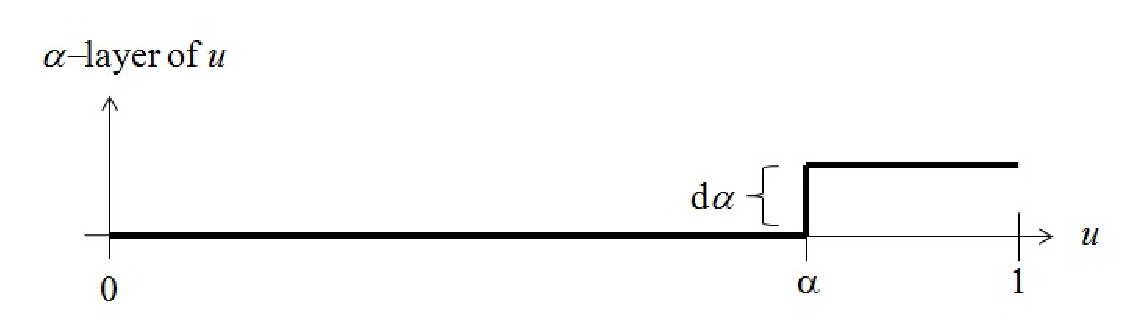
\includegraphics{layer.eps}}
    \end{tabular}
    \caption{Illustration of $\alpha$-layer of $u$, written as $I_\alpha(u)\de \alpha$. The $\alpha$-layer of $u$ is only sensitive to movements in $u$ at $\alpha$ and ignores other movements.  }
    \label{flayer}
  \end{center}
\end{figure}


As often exploited  in reinsurance, any non-negative random loss or variable can be thought of as a sum of layers. Applying this concept to $u$ yields
\begin{equation}\label{decompose}
u=\int_0^u 1\de \alpha= \int_0^1 I_\alpha(u)\de\alpha    \;.
\end{equation}
Hence $u$ is formed from infinitely many layers, each capturing the movement of $u$ at a particular value.


\subsection{Constructing layer dependence}

Spearman's correlation is the correlation and also the standardized covariance between two percentile rank random variables $v$ and $u$:
$$
\rho \equiv \cor(u,v) = \frac{\cov(v,u)}{\cov(u,u)}
$$
where $\cor$ and $\cov$ indicate covariance and correlation, respectively. In the final expression, the denominator $\cov(u,u)=1/12$ is a constant and a scaling factor ensuring $\rho=1$ if $u=v$ that is $u$ and $v$ are comonotonic. The numerator $\cov(v,u)$ reveals the overall dependence between $v$ and $u$, and is rewritten as, using the decomposition of $u$ in \eref{decompose},
\begin{equation}\label{spearman}
\cov(v,u)=\cov\left\{v,\int_0^1I_\alpha(u)\de \alpha \right\}= \int_0^1 \cov\{v,I_\alpha(u)\} \de \alpha \; .
\end{equation}
Therefore the covariance $\cov(v,u)$ is decomposed into infinitely many covariances $\cov\{v,I_\alpha(u)\}$ for $0\le\alpha\le 1$. Each covariance measures the dependence between $v$ and the $\alpha$--layer of $u$. In a reinsurance setting, this covariance measures dependence between a particular layer of a loss (in percentile rank terms) and another factor. Alternatively the covariance captures dependence between $v$ and movements in $u$ at $\alpha$. Both interpretations point to $\cov\{v,I_\alpha(u)\}$ as a measure of local dependence between $v$ and $u$. Similar to $\rho$, scaling this covariance with the same when $v=u$ leads to the definition of layer dependence
\begin{equation}\label{ellalpha}
\ell_\alpha \equiv \frac{\cov\{v,I_\alpha(u)\}}{\cov\{u,I_\alpha(u)\}}   \;,
\end{equation}
where the denominator 
$$
\cov\{u,I_\alpha(u)\}=\E\{uI_\alpha(u)\}-\E(u)\E\{I_\alpha(u)\}=\int_\alpha^1 u \de u - 0.5\int_\alpha^1 1 \de \alpha
$$
$$
=0.5\alpha(1-\alpha) \;.
$$
where $\E$ calculates expectations. 

It is shown that if $\ell_\alpha=1$ for any $\alpha$ then $u$ and $v$ crosses $\alpha$ simultaneously: perfect dependence at $\alpha$. In addition $\ell_\alpha=1$ over $c\le\alpha\le d$ implies $u=v$ over $c\le u,v\le d$. The equality weakens as $\ell_\alpha$ decreases. These results are illustrated and formalised in \sref{sldcurve} and \sref{sdecompose} respectively.

Combining \eref{spearman} and \eref{ellalpha} yields
\begin{equation}\label{wtdavg}
\rho = \int_0^1 \ell_\alpha \frac{\cov\{u,I_\alpha(u)\}}{\cov(u,u)} \de \alpha =  \int_0^1 \ell_\alpha 6\alpha(1-\alpha) \de \alpha \; .
\end{equation}
Hence $\rho$ is a weighted average of $\ell_\alpha$ across $0\le\alpha\le 1$ with weights $w_\alpha=6\alpha(1-\alpha)$ integrating to $1$. This result is consistent with the fact that $\rho$ measures overall dependence whereas $\ell_\alpha$ decomposes $\rho$ into local dependence values. Note $w_\alpha$ has minimum $0$ at $\alpha=0$ and $1$, and increases symmetrically to maximum at $\alpha=0.5$. Hence Spearman's correlation places less emphasis on the tails which may be undesirable in finance or insurance where tail dependence is critical. Modifying the weights $w_\alpha$ leads to alternate measures of overall dependence further explored in \sref{saltoverall}.


Layer dependence summaries the dependence structure of a copula. Layer dependence provides an additional dimension of information compared to Spearman's correlation. As for any summary measure, layer dependence can mislead but is less misleading than $\rho$ and other measures of overall dependence. Layer dependence is also a more meaningful characterisation of a copula compared to the parameters of copula families such as the Clayton or Gumbel \citep{mcneil2005qrm}. Properties of and arguments for using layer dependence are explored below.


This paper assumes exchangeability: $C(u,v)=C(v,u)$ where $C$ is the copula of $(u,v)$. Hence $u$ and $v$ can be interchanged in the above expressions and those remaining in this paper. Archimedean copulas are a well known class of exchangeable copulas \citep{mcneil2005qrm}.



\subsection{Key properties of layer dependence}

Layer dependence $\ell_\alpha$ satisfies the following coherence properties for all $0\le\alpha\le 1$. These properties are shared with Spearman's correlation and are formalised in \sref{scoherence}. Similar to correlation, $0\le\ell_\alpha\le 1$, and $\ell_\alpha=-1$, $0$ and $1$ if $u$ and $v$ are countermonotonic, independent and comonotonic, respectively. In addition $\ell_\alpha$ increases with the correlation order of $(u,v)$. Replacing $u$ or $v$ with their complement leads to straightforward changes in layer dependence.

The following is an alternative expression of $\ell_\alpha$:
\begin{equation}\label{gapexp}
\ell_\alpha = \frac{\E(v|u>\alpha)-\E(v|u\leq \alpha)}{\E(u|u>\alpha)-\E(u|u\leq \alpha)}
=2 \left\{\E(v|u>\alpha)-\E(v|u\leq \alpha)\right\}\;.
\end{equation}
A proof is shown in the appendix. The middle expression in \eref{gapexp} is the expected change in $v$ relative to the expected change in $u$ when $u$ crosses $\alpha$. The latter is $0.5$ for all $\alpha$, yielding the final expression in \eref{gapexp}. Hence large $\ell_\alpha$ implies $v$ is sensitive to movements in $u$ across $\alpha$, indicating strong dependence between $v$ and $u$ at $\alpha$. When $\ell_\alpha=0$, $v$ is unchanged on average when $u$ crosses $\alpha$, hence $u$ and $v$ are not dependent at $\alpha$.




\begin{comment}
  Further alternative expressions are
$\ell_\alpha = (\tau_\alpha-1)/\alpha$ and $\tau_\alpha= (1+\alpha\ell_\alpha)/2$
where  $\tau_\alpha\equiv \E(v|u>\alpha)$.  These  alternative expressions for $\ell_\alpha$ follow from
$$
\cov\{v,(u>\alpha)\} =\frac{(2\tau_\alpha-1)(1-\alpha)}{2}
\cq
\cov\{u,(u>\alpha)\} =\frac{\alpha(1-\alpha)}{2}\ .
$$

Further
$$
\cor\{v,(u>\alpha)\}=\frac{\cov\{v,(u>\alpha)\}}{\sqrt{\alpha(1-\alpha)/12}}  = \ell_\alpha \sqrt{3\alpha(1-\alpha)}\ .
$$
\end{comment}



\section{Illustration of layer dependence curves for various copulas}\label{sldcurve}

The nine panels in \fref{fillustration} display $(u,v)$ scatterplots of well known exchangeable copulas. Less standard copulas are also shown for illustration. All copulas are calibrated to have equal Spearman's correlation $\rho=0.6$. Layer dependence curves $\ell_\alpha$ for all $0\le\alpha\le 1$ are plotted against $\alpha$ on $(u,v)$ scatterplots to demonstrate the link between the scatter and $\ell_\alpha$.

The scatterplots in \fref{fillustration}  emphasize that copulas with the same overall dependence can exhibit a variety of local dependence structures and these structures are captured by layer dependence curves. Given $\alpha$, $\ell_\alpha$ is larger if scatter points are more clustered around $(\alpha,\alpha)$ and vice versa. In particular $\ell_\alpha$ increases to one in the tails of copulas exhibiting strong tail dependence. Hence $\ell_\alpha$ tracks the clustering of scatter points across the $45\circ$ line. This observation is formalised in \sref{sdecompose}.

\begin{figure}
  \begin{center}
    \begin{tabular}{ccc}
      \resizebox{40mm}{!}{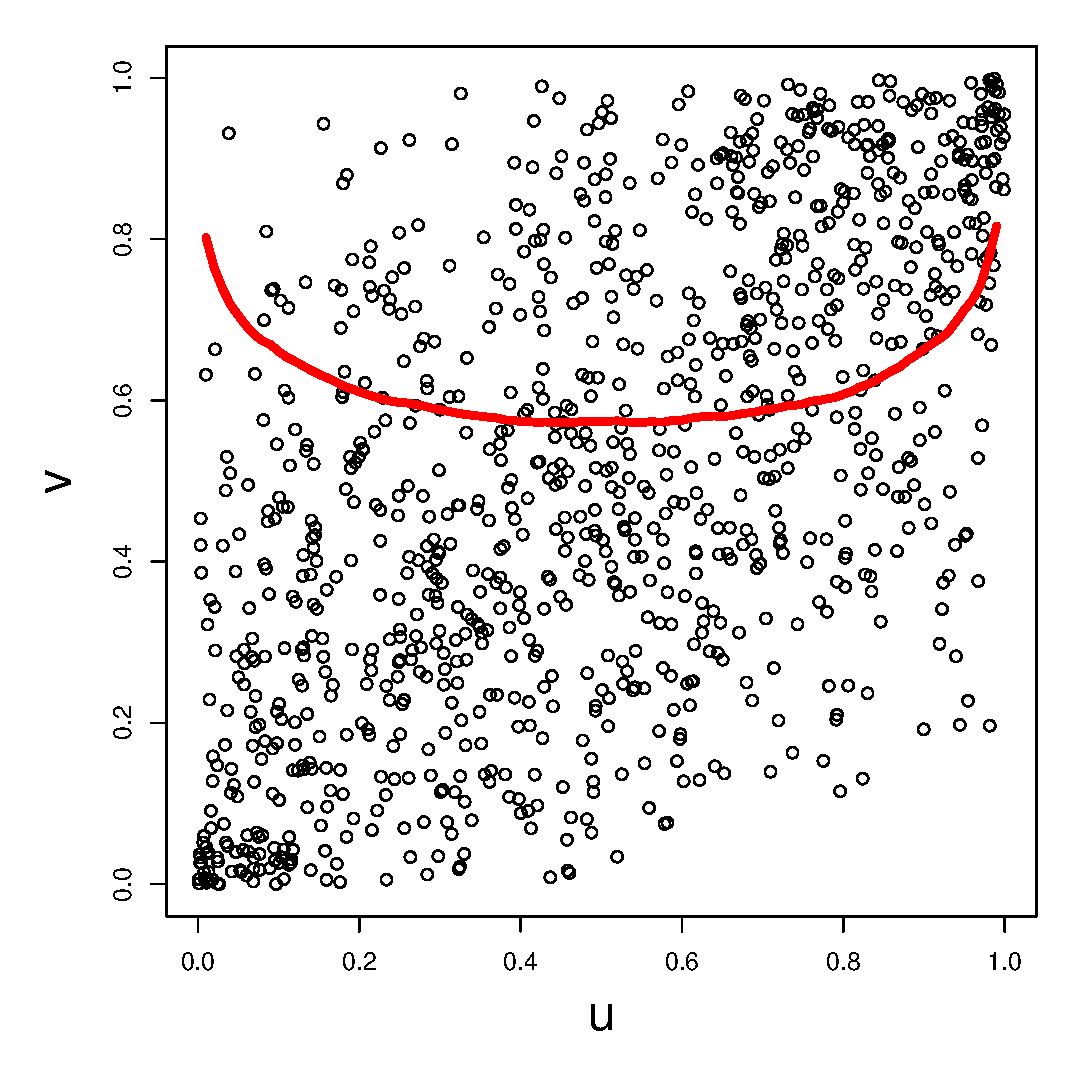
\includegraphics{normal.eps}}
            \resizebox{40mm}{!}{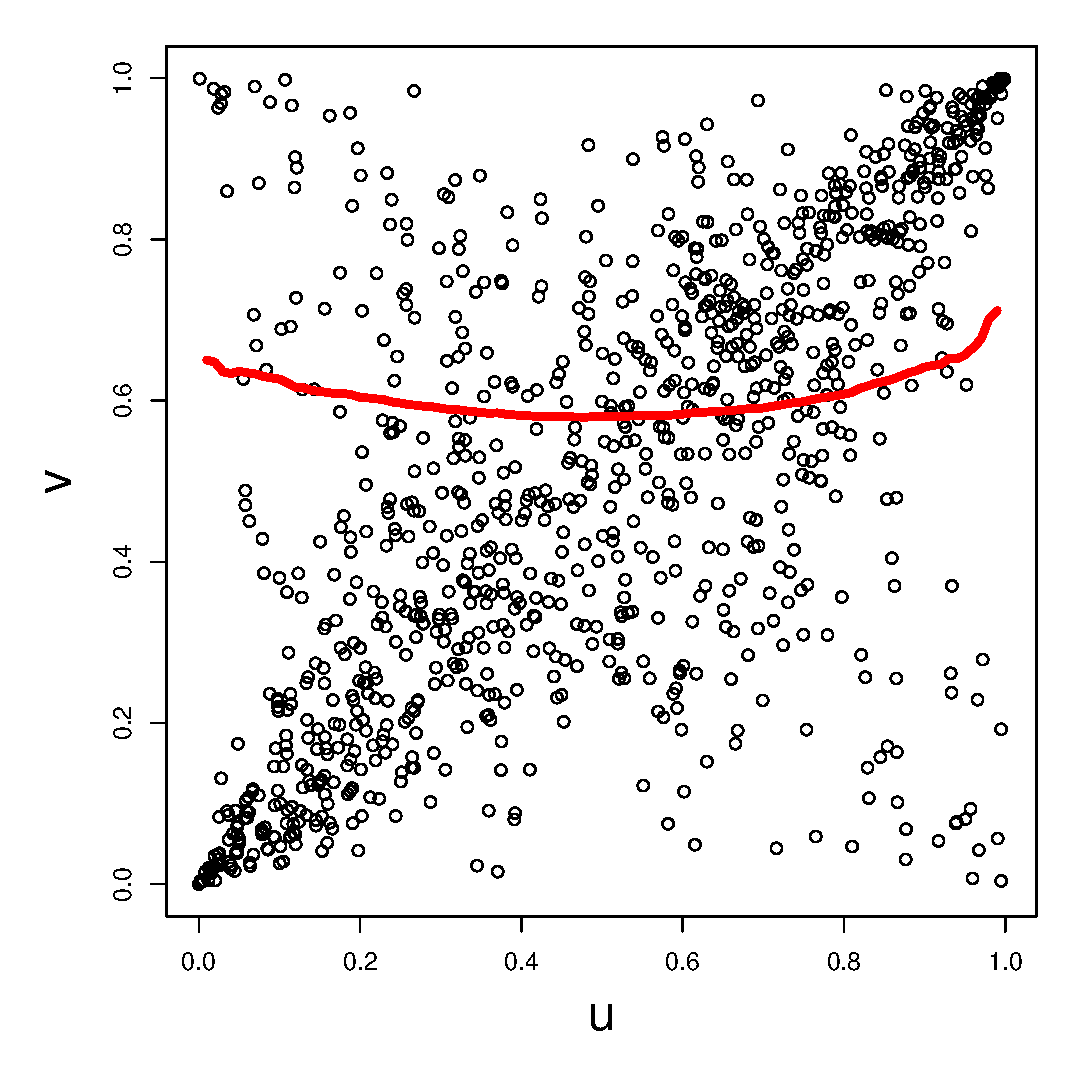
\includegraphics{student.eps}}
      \resizebox{40mm}{!}{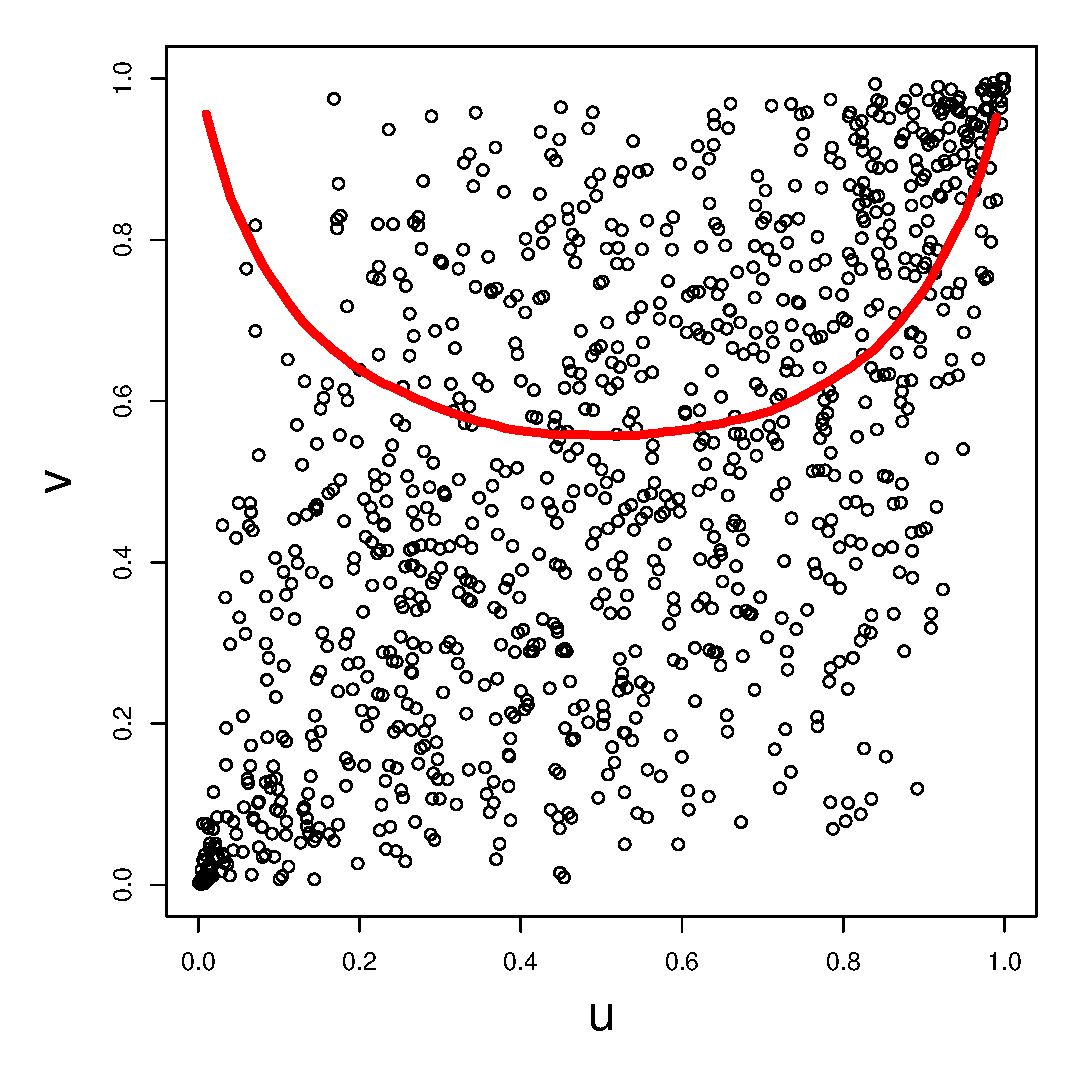
\includegraphics{structural2.eps}} \\
      \resizebox{40mm}{!}{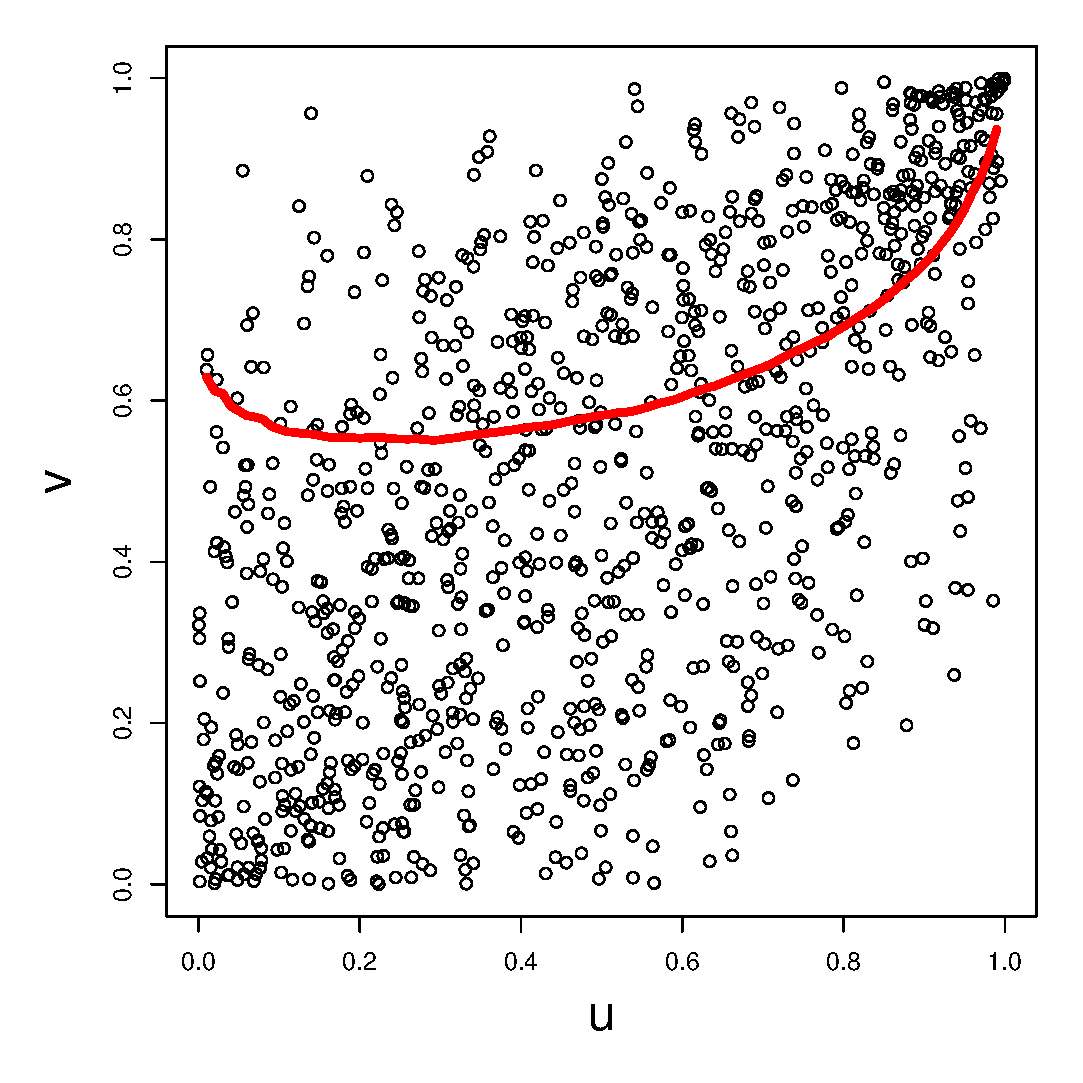
\includegraphics{gumbel.eps}}
            \resizebox{40mm}{!}{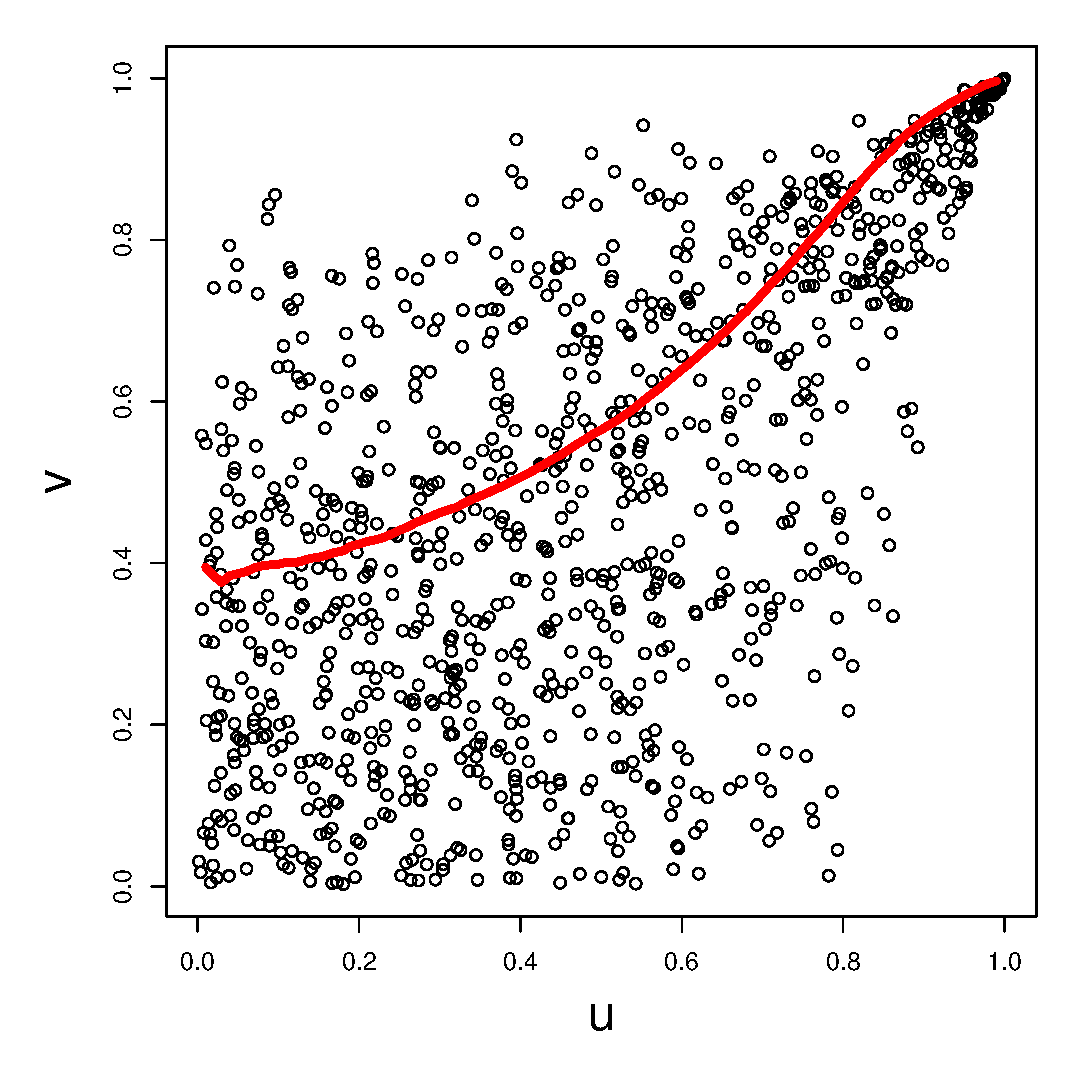
\includegraphics{structural1.eps}}
      \resizebox{40mm}{!}{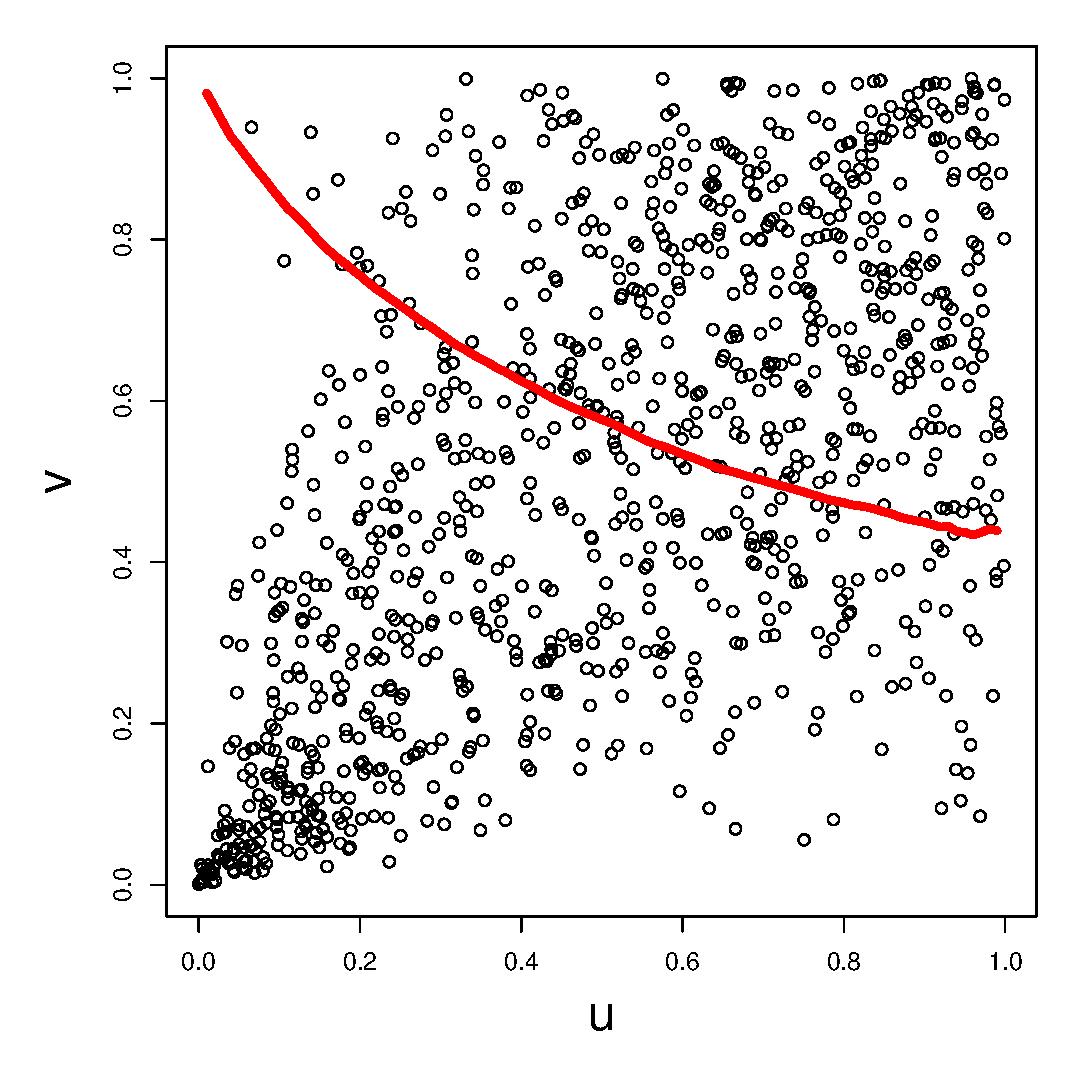
\includegraphics{clayton.eps}} \\
            \resizebox{40mm}{!}{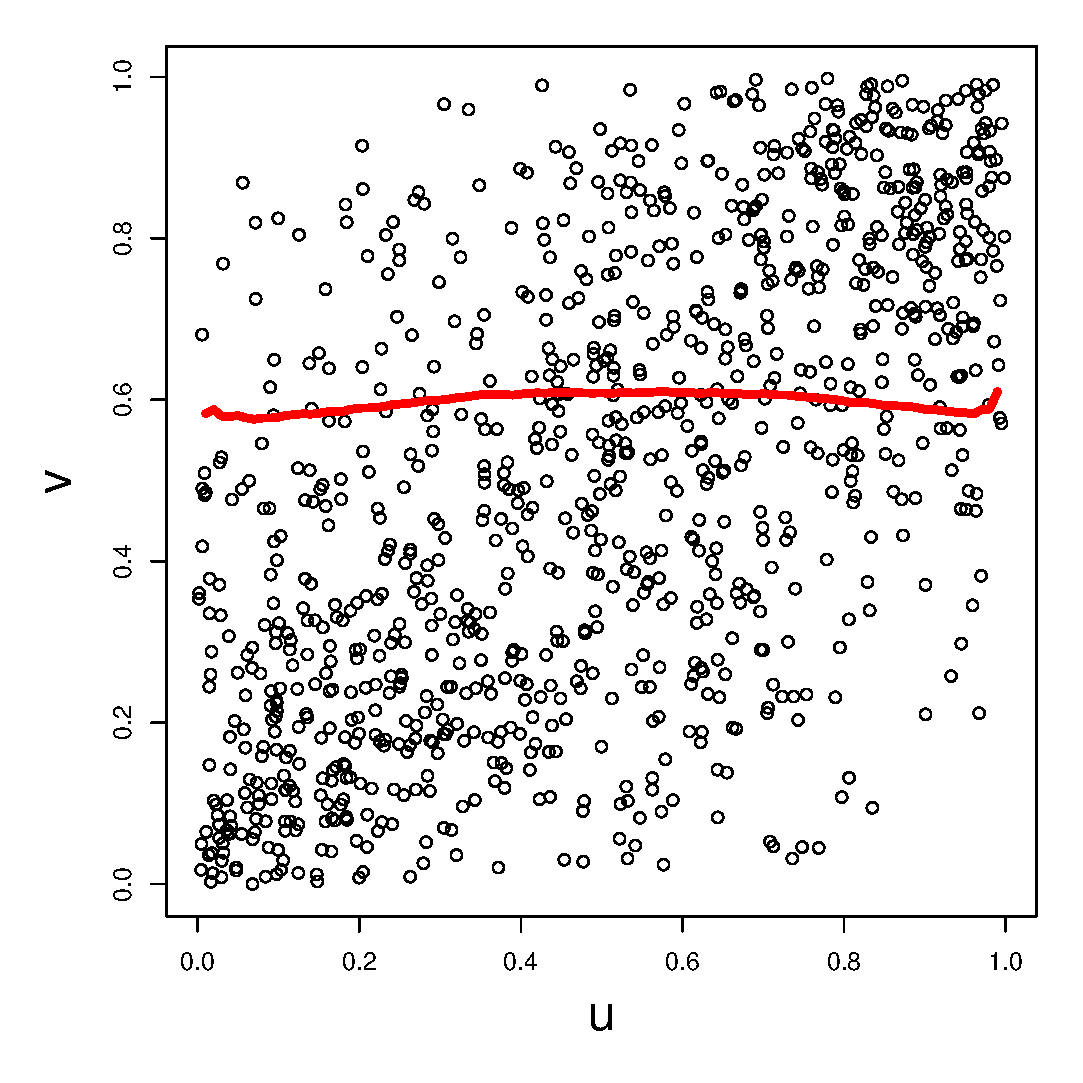
\includegraphics{frank.eps}}
            \resizebox{40mm}{!}{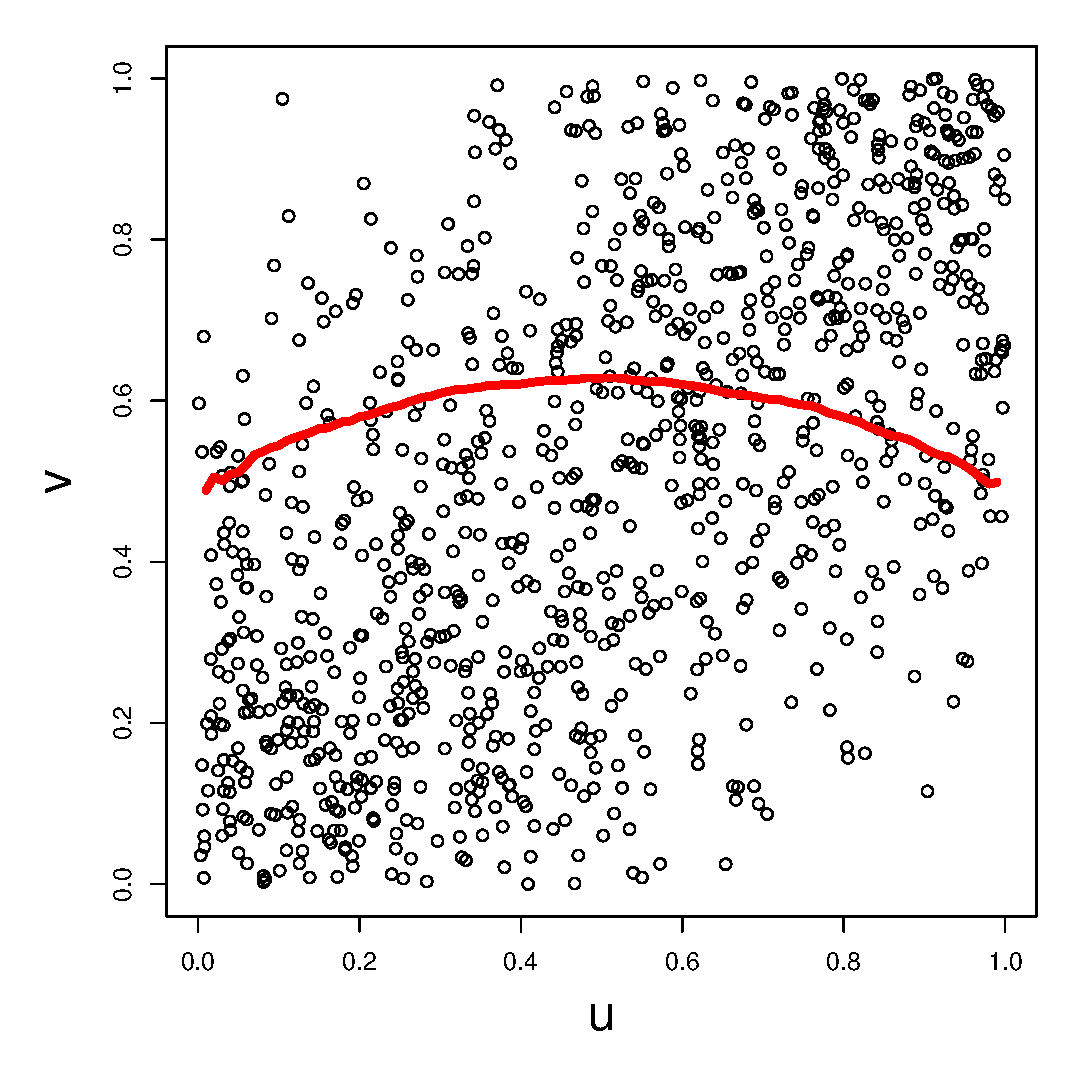
\includegraphics{structural3.eps}}
      \resizebox{40mm}{!}{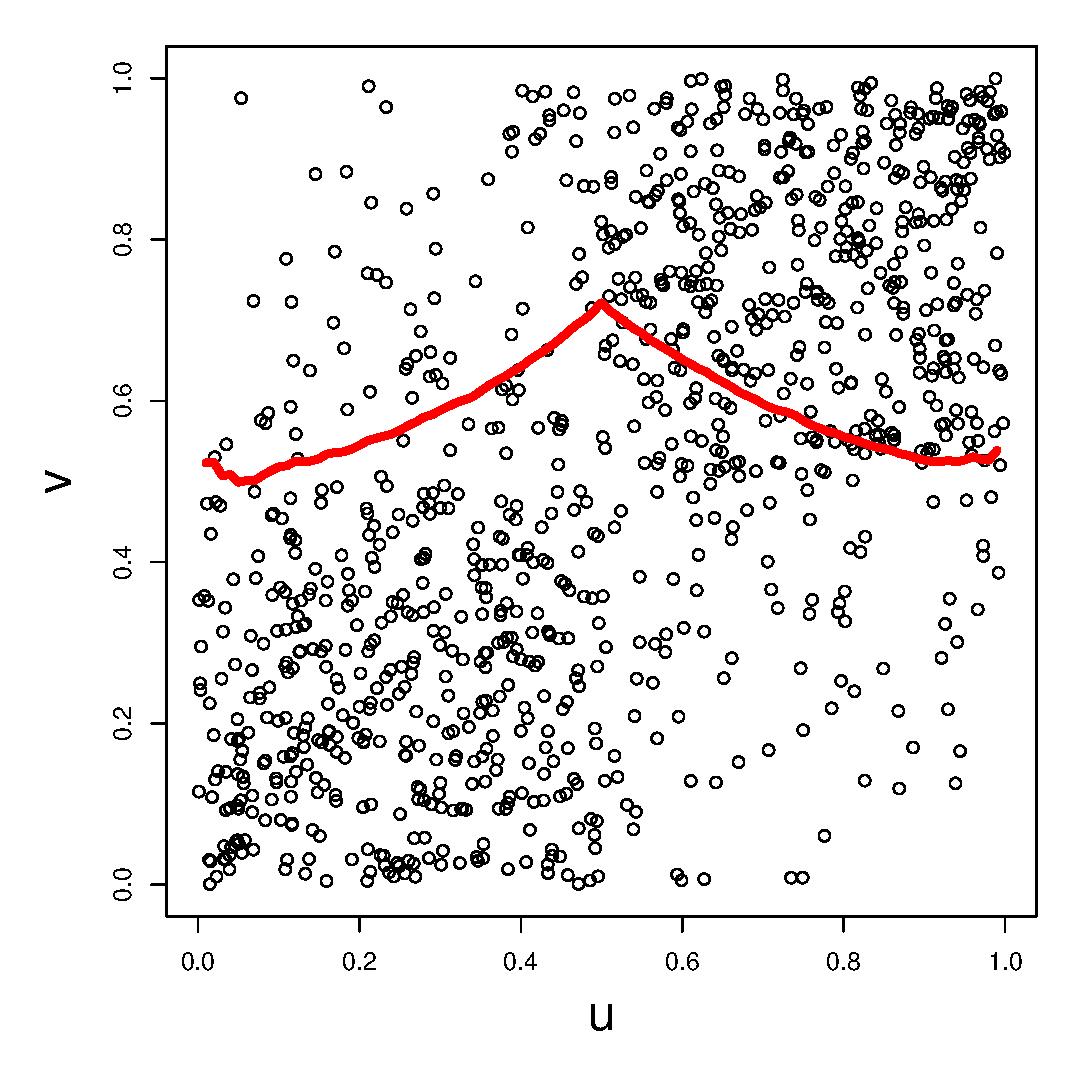
\includegraphics{structural4.eps}} \\
    \end{tabular}
    \caption{Copulas all with the same $\rho=0.6$ but different layer dependence curves $\ell_\alpha$ over $0\leq\alpha\le 1$ (in red). The top 3 copulas display relatively strong tail dependence in both lower and upper tail.  The first two copulas in the middle three have relatively strong upper tail dependence and while the third has a high degree of lower tail dependence. The bottom three copulas have relatively high local dependence in the middle of the distribution and less correlation in the tails. Overall the panels illustrate how a given overall level of $\rho$ can mask a range of dependence structures and that layer dependence is an appropriate tool for assessing local dependence. The top left panel displays a Gaussian copula, followed by a Student's $t$ copula on the right. The leftmost panel in the middle three is a Gumbel copula, and the rightmost is a Clayton copula. The bottom left panel is a Frank copula. Remaining copulas are constructed from a factor model and are included to illustrate how layer dependence captures local dependence.}
    \label{fillustration}
  \end{center}
\end{figure}



\section{Layer dependence, discordance and dispersion}\label{sdecompose}

As before assume the copula of $(u,v)$ is exchangeable. The following result shows a negative relationship between layer dependence at any point and discordance and dispersion of $(u,v)$ relative to the same point. This result explains the behaviour of layer dependence curves in \fref{fillustration} where $\ell_\alpha$ increases as $(u,v)$ become scattered more closely around $(\alpha,\alpha)$, that is lower discordance and dispersion.

Layer dependence $\ell_\alpha$ can be written as
\begin{equation}\label{decomposition}
\ell_\alpha = 1-2(1+\gamma_\alpha) \delta_\alpha \;,
\end{equation}
where
$$
\gamma_\alpha \equiv \cor\{1-I_\alpha(u),I_\alpha(v)\} =\cor\{I_\alpha(u),1-I_\alpha(v)\}=\frac{\alpha^2-C(\alpha,\alpha)}{\alpha(1-\alpha)}\;,
$$
and
$$
\delta_\alpha \equiv\E\left\{(|u-v|)|(u-\alpha)(v-\alpha)<0\right\}  \; .
$$
A proof of \eref{decomposition} is shown in the appendix. The correlation $-1\leq\gamma_\alpha\leq 1$ measures the tendency for $(u,v)$ to be discordant at $\alpha$: either $u$ or $v$ is above $\alpha$ and the other is below $\alpha$. The expectation $0\leq \delta_\alpha\leq 1$ measures the average dispersion between discordant $u$ and $v$ at $\alpha$, noting $(u-\alpha)(v-\alpha)<0$ is equivalent to $u>\alpha$ and $v\le\alpha$ or $u\le\alpha$ and $v>\alpha$.


\fref{finterpretation} illustrates \eref{decomposition} using two copulas specifically constructed such that, for $\alpha=0.75$, $\ell_\alpha=1$ for one and $\ell_\alpha=0.86$ for the other. For the copula where $\ell_\alpha=1$, there is no discordance or dispersion at $\alpha$. This observation is confirmed by setting $\ell_\alpha=1$ in \eref{decomposition} yielding $\gamma_\alpha=-1$ or $\delta_\alpha=0$. In this case $u$ and $v$ are perfectly dependent at $\alpha$, and are simultaneously below or above $\alpha$. It is also straightforward to extend this result such that if $\ell_\alpha=1$ over $c\le\alpha\le d$ then $u=v$ over $c\le u,v\le d$. As $\ell_\alpha$ decreases from $1$, as for the second copula, the extent of discordance $\gamma_\alpha$ and dispersion $\delta_\alpha$ increases. Again this result can be confirmed from \eref{decomposition} noting $\ell_\alpha$ is negatively related to $\gamma_\alpha$ and $\delta_\alpha$.


\begin{figure}
  \begin{center}
    \begin{tabular}{cc}
      \resizebox{60mm}{!}{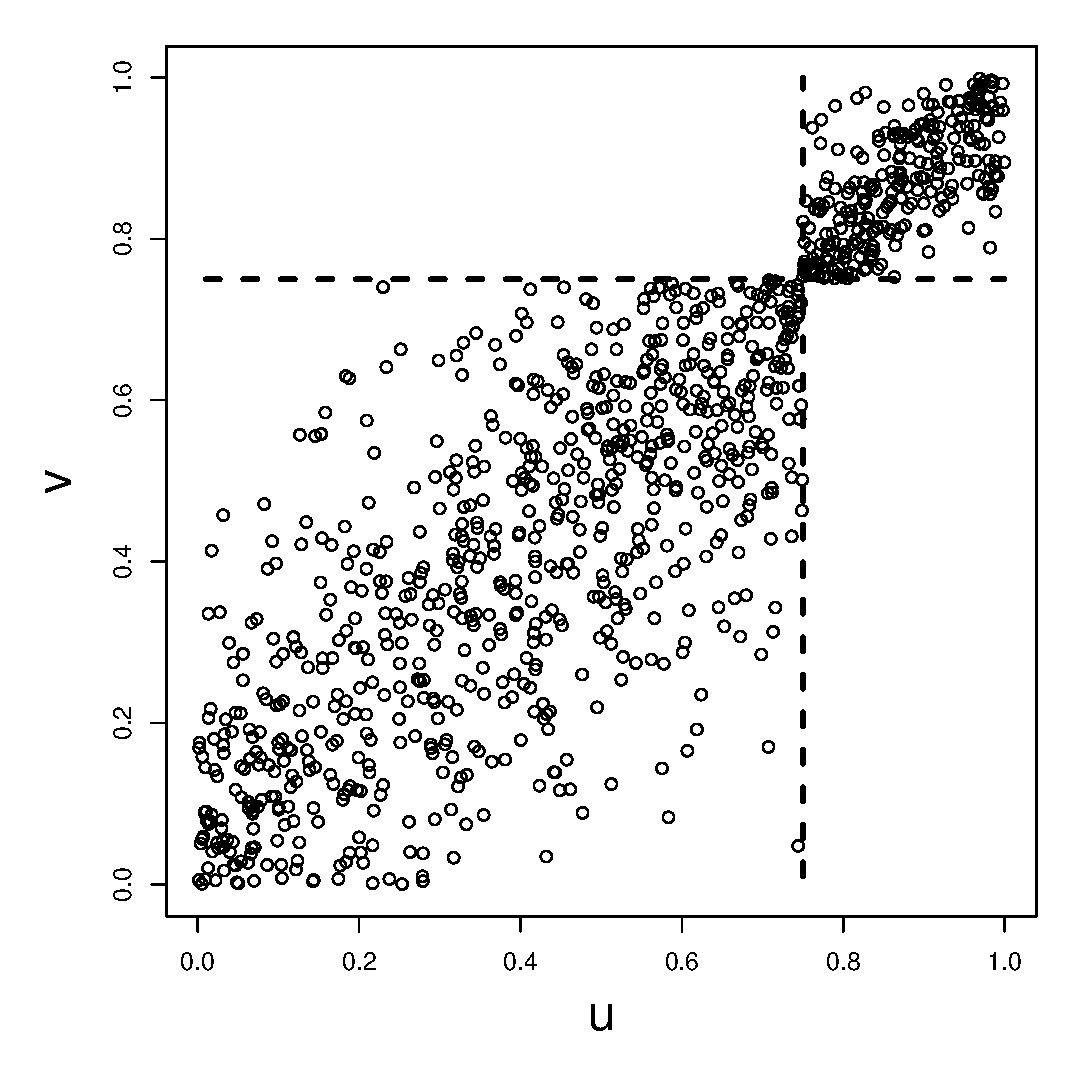
\includegraphics{perfect.eps}}
      \resizebox{60mm}{!}{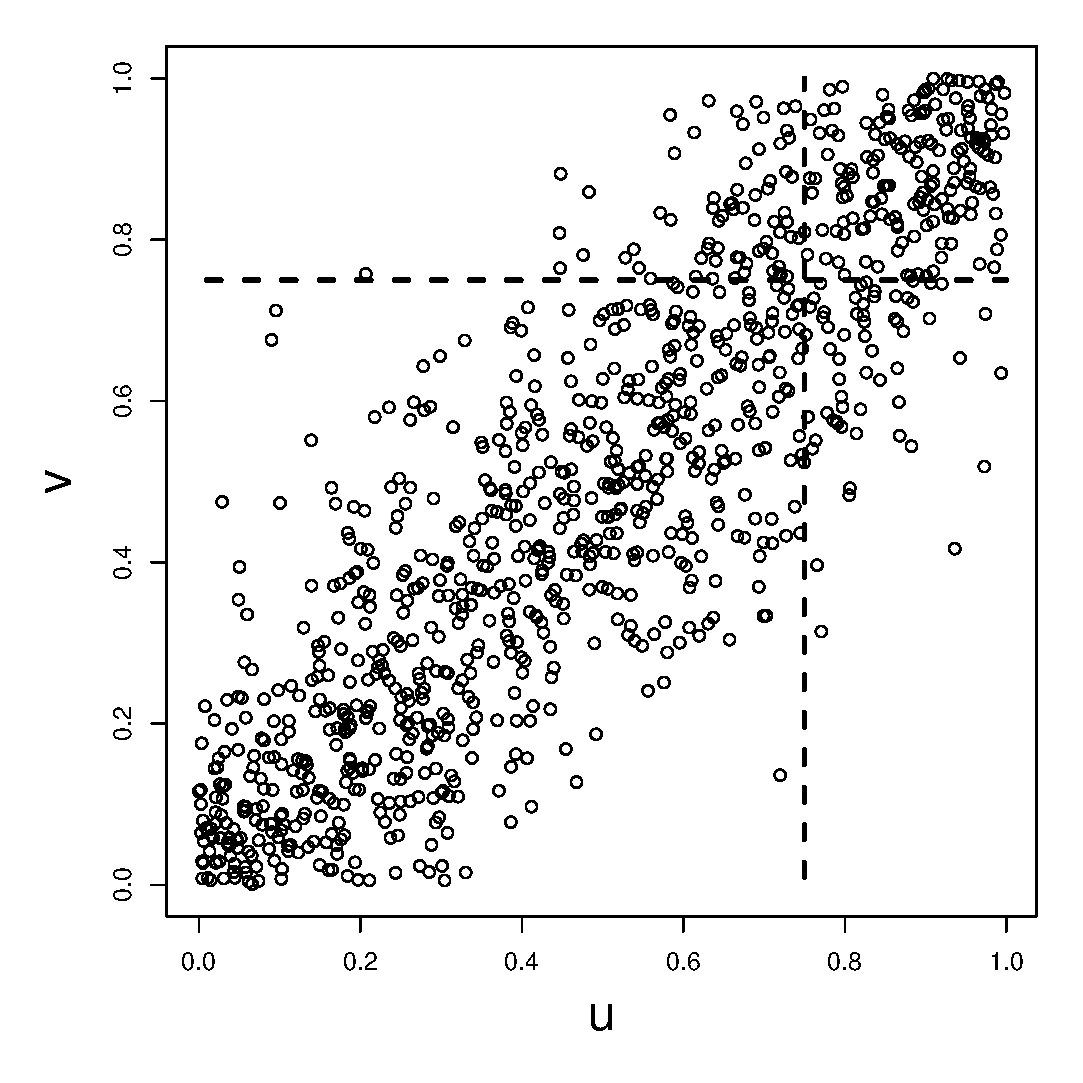
\includegraphics{imperf.eps}} \\
    \end{tabular}
    \caption{The left and right panel show copulas where $\ell_{0.75}=1$ and $\ell_{0.75}=0.86$, respectively. In the left panel, $\gamma_{0.75}=-1$ (no discordant points) and $\delta_{0.75}=0$ (zero dispersion). In the right panel, $\gamma_{0.75}=-0.65$ (some discordant points) and $\delta_{0.75}=0.21$ (some dispersion between discordant points). }
    \label{finterpretation}
  \end{center}
\end{figure}


The result in \eref{decomposition} explains the behaviour of layer dependence curves in \fref{fillustration}. Layer dependence $\ell_\alpha$ is larger if scatter points are more clustered around $(\alpha,\alpha)$, that is, fewer discordant points at $\alpha$, and discordant points at $\alpha$ are closer to the $45^\circ$ degree line. The former indicates smaller $\gamma_\alpha$ and the latter indicates smaller $\delta_\alpha$. Opposite observations apply for small $\ell_\alpha$.





\begin{comment}

The probability of discordance is
$$
\E[\{(u-\alpha)(v-\alpha)<0\}]
=2\alpha\{(1-\alpha)(\gamma_\alpha+\alpha^2)-1\} \;.
$$


The following illustrates \eref{decomposition} using the income-education example introduced in \sref{sintroduction}. Given $\alpha$, classify individuals as ``concordant" or ``discordant." The former are those with income and education both below or above $\alpha$. The latter are remaining individuals. Scale the proportion of concordant individuals to yield $\gamma_\alpha^*$. Calculate average dispersion $\delta_\alpha$ as twice the average difference between income and education of discordant individuals. Combine $\gamma^*_\alpha$ and $\delta_\alpha$ using \eref{decomposition} to yield $\alpha$-layer dependence $\ell_\alpha$. Layer dependence decreases with the proportion of discordant individuals and their average income-education dispersion.




\fref{fdecomposition} illustrates the decomposition of percentile rank gap by separately showing the standardised concordance probability $\gamma_\alpha^*$ and dispersion $\delta_\alpha$. The same four copulas as in \fref{fillustration} are applied.

\begin{figure}
  \begin{center}
    \begin{tabular}{cc}
      \resizebox{60mm}{!}{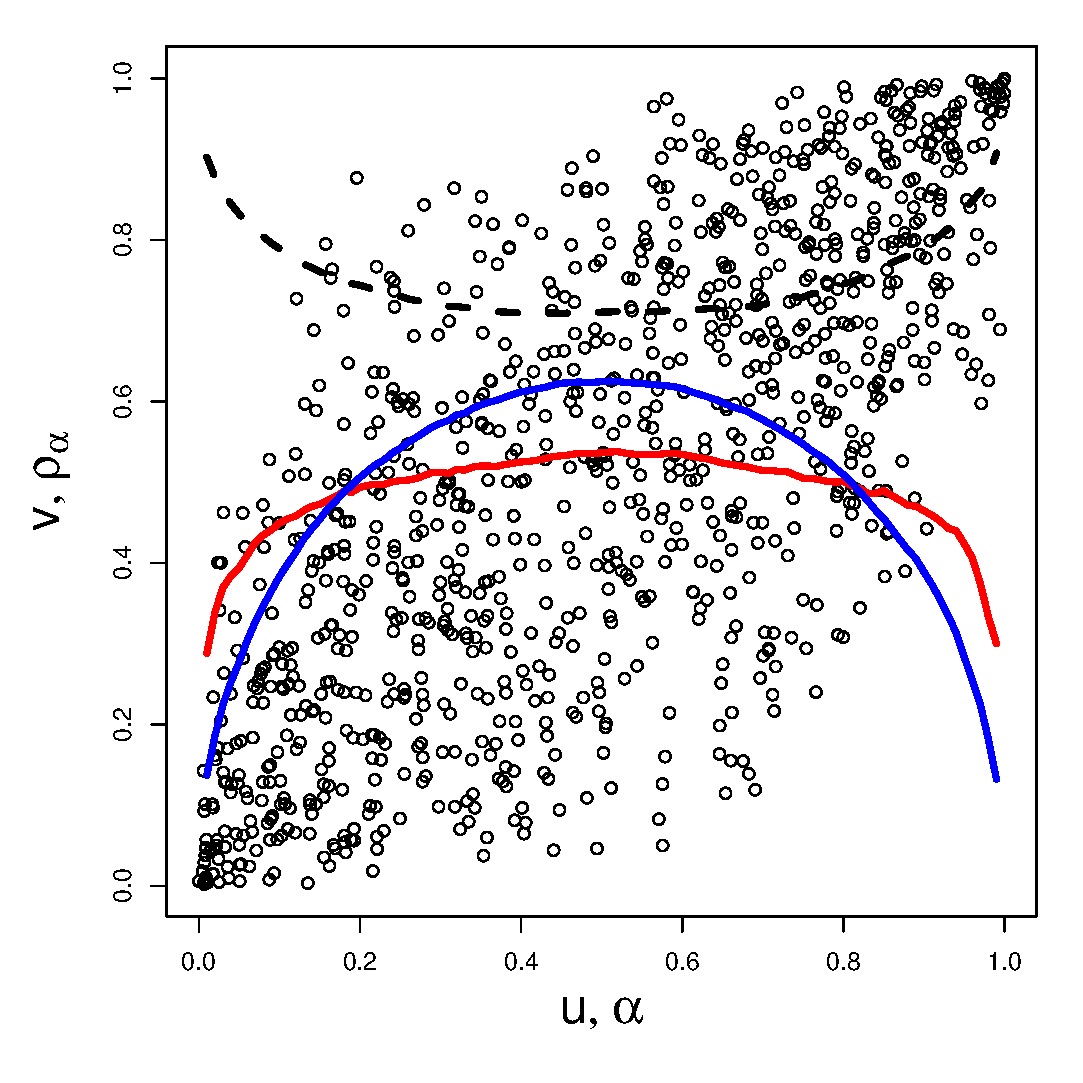
\includegraphics{normaldecom.eps}}
      \resizebox{60mm}{!}{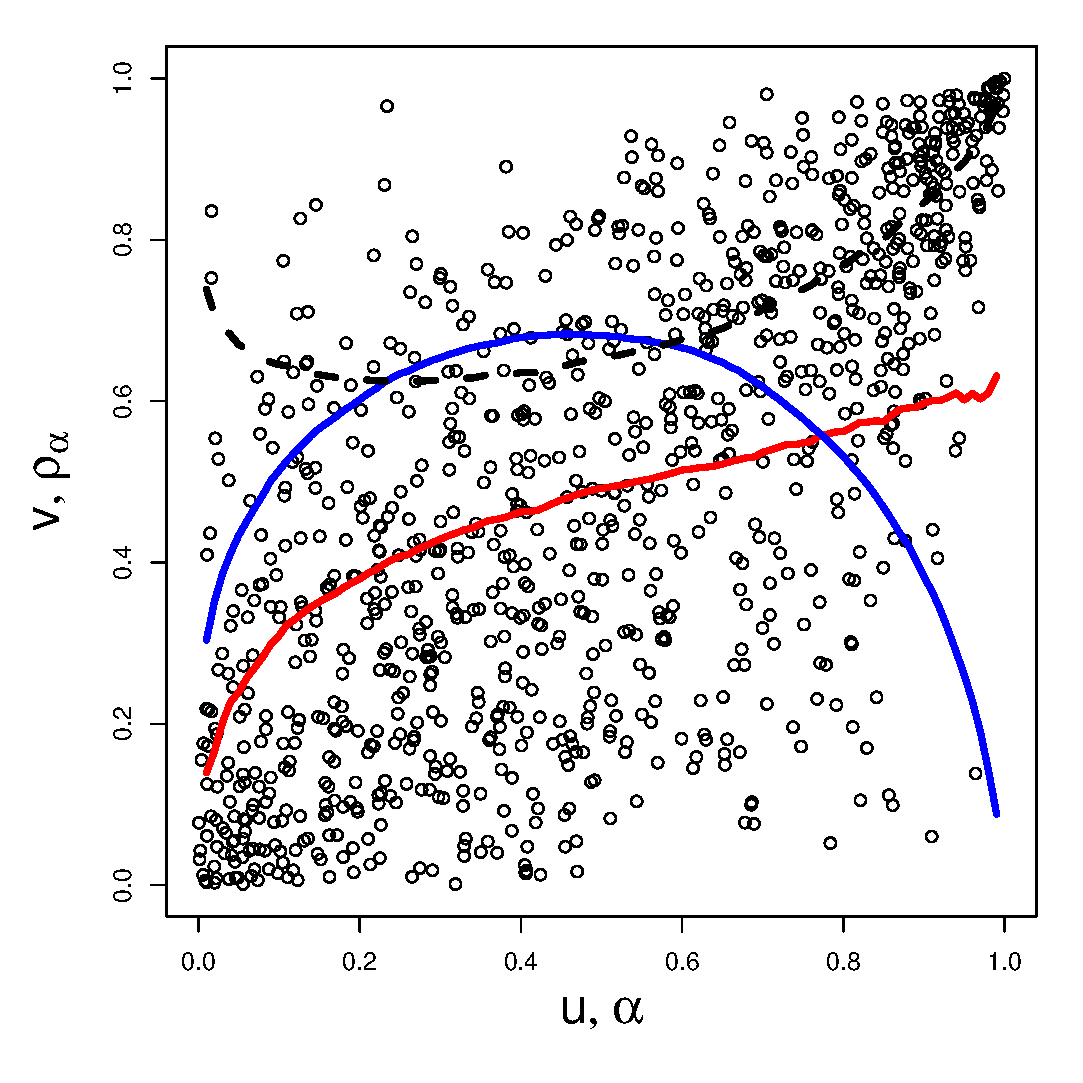
\includegraphics{gumbeldecom.eps}} \\
      \resizebox{60mm}{!}{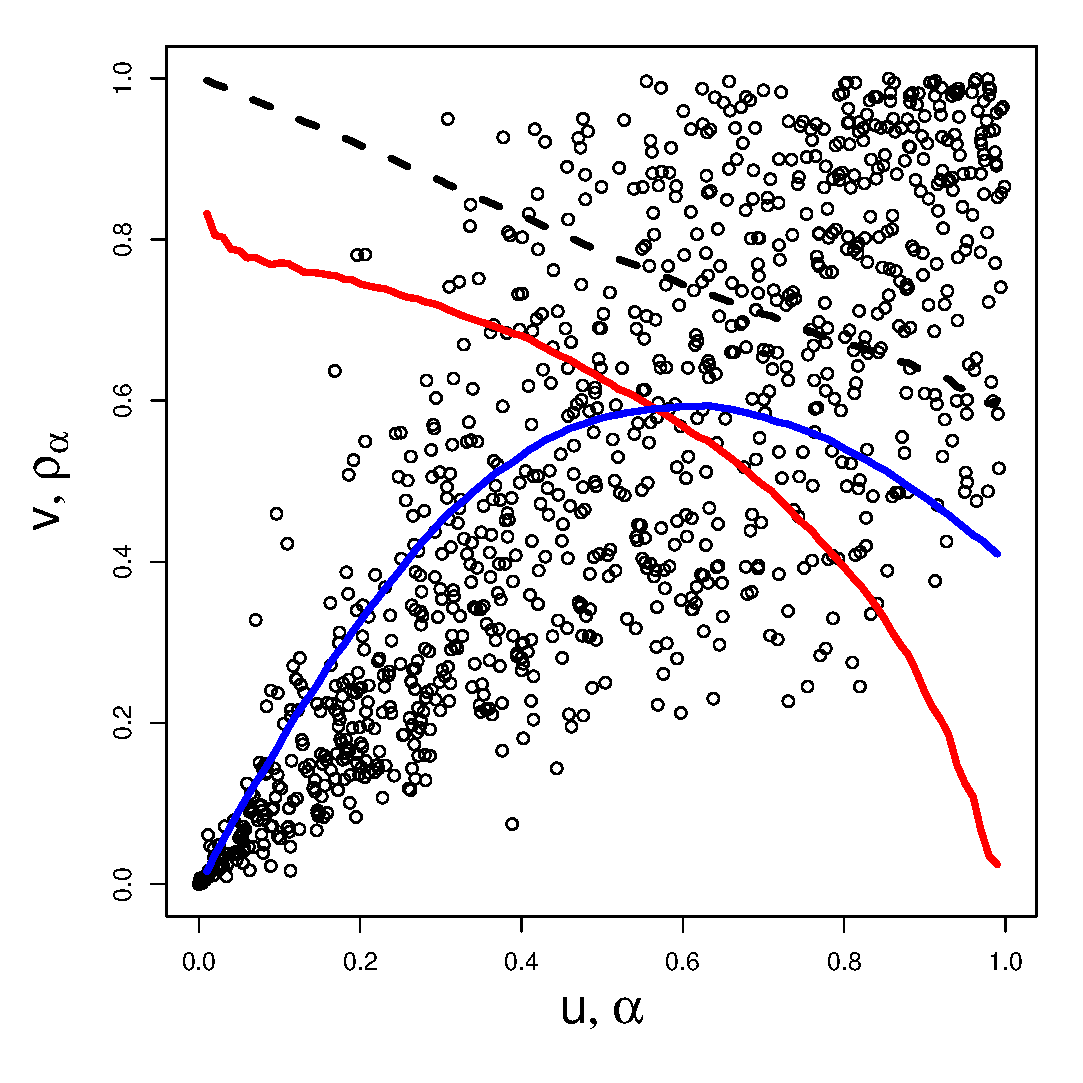
\includegraphics{claytondecom.eps}}
      \resizebox{60mm}{!}{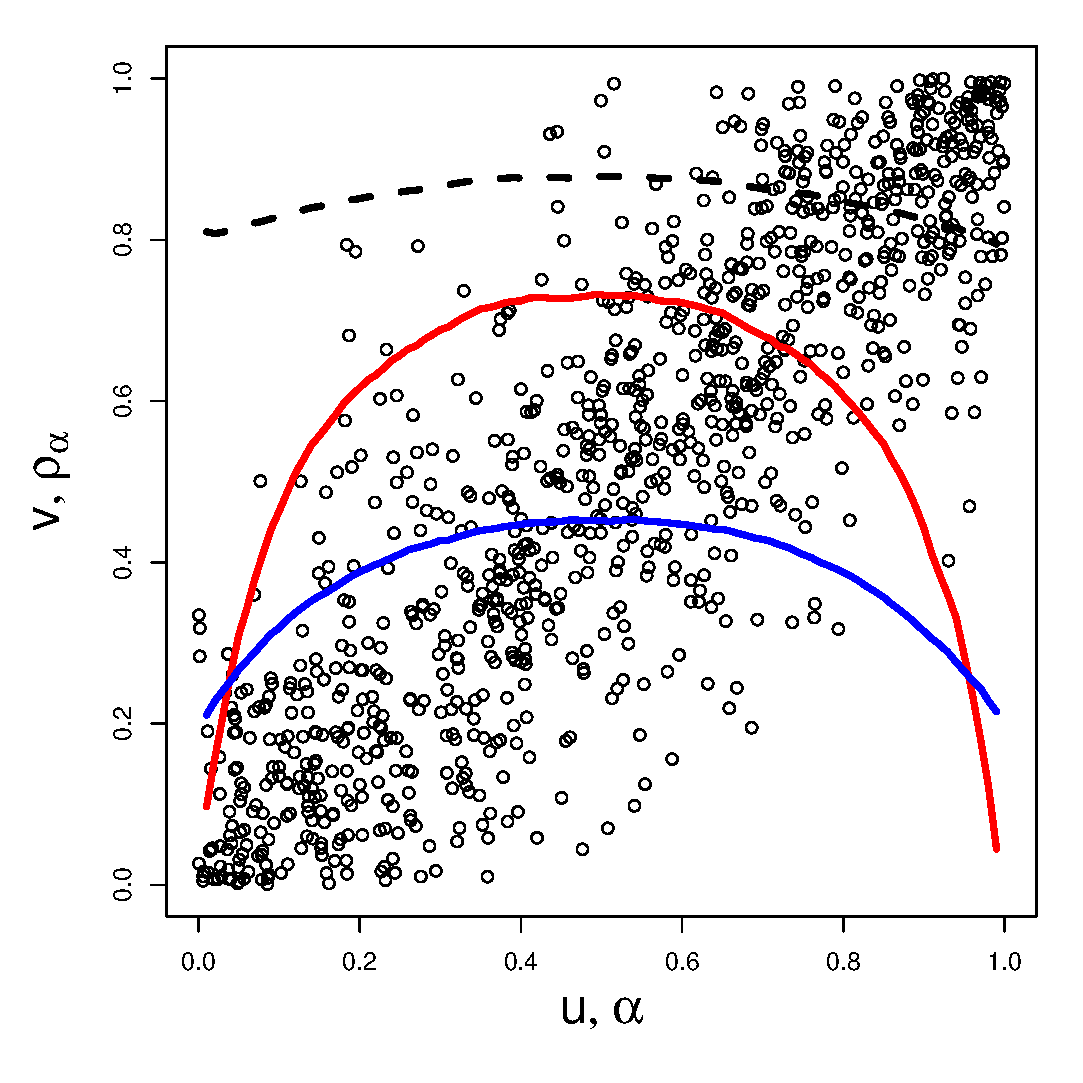
\includegraphics{frankdecom.eps}} \\
    \end{tabular}
    \caption{Standardised concordance probability $\sgamma^*_\alpha$ (red line) and dispersion $\delta_\alpha$ (blue line) for a Gaussian copula (top left), Gumbel copula (top right), Clayton copula (bottom left) and Frank copula (bottom right). Percentile rank gap (dotted black line) is also shown.}
    \label{fdecomposition}
  \end{center}
\end{figure}



Manipulating the expression for $\ell_\alpha$ in \eref{relationship} yields
$$
\ell_\alpha = 1- \frac{\E\{d(u,v) z_\alpha\}}{\alpha(1-\alpha)}  \cq \ell = 1-6\int_0^1 \E\{d(u,v)z_\alpha\} \de \alpha \;.
$$
where the above result for $\ell$ applies $\ell=\int_0^1 w_\alpha \ell_\alpha \de \alpha$, $w_\alpha\equiv 6\alpha(1-\alpha)$. Hence $\rho_S$ is negatively related to the average dispersion between discordant $(u,v)$ over all $\alpha$.






========== Haven't done much below here =============

\subsection{Income-education interpretation}

The following interprets layer dependence using an income-education example. Consider education $(u)$ and income $(v)$ rankings of individuals in a population, with $0$ and $1$ representing lowest and highest, respectively. Given $\alpha$, divide the population into two segments based on education: $u\leq \alpha$ and $u>\alpha$. Measure average income in each segment. From \eref{gapexp}, $\alpha$-layer dependence is twice the gap in average income between the two segments.

Suppose $\ell_\alpha$ is close to one for $\alpha=0.95$. This implies highly educated individuals (top $5\%$) are likely to be high income earners (top $5\%$), and vice versa. Few individuals have top $5\%$ education and income not in top $5\%$ or vice versa, and their average education-income difference is small. Hence there is strong income-education dependence at the $95$th percentile education layer. Dependence is perfect if $\ell_\alpha=1$. If $\ell_\alpha=0$ then average income is equal between individuals with education below and above top $5\%$, implying independence at the $95$th percentile education layer. The same argument applies to $\ell_\alpha$ for other values of $\alpha$.

This paper formulates layer dependence in terms of $u$ and $v$, in this case income and education ranks. Section \sref{soriginal} discusses an analogous definition of layer dependence between observed random variables $x$ and $y$, or original measurements of income and education.

\end{comment}





\section{Coherence properties of layer dependence}\label{scoherence}


Layer dependence $\ell_\alpha$ satisfies the following five ``coherence" properties. These properties are extensions of properties applying to Spearman's correlation. 
\begin{itemize}

\item \textbf{Bounds}: Layer dependence lies between $-1$ and $1$: $-1 \le\ell_\alpha \le 1$ for all $\alpha$.
Hence layer dependence is bounded in the same way as $\rho$.

\item \textbf{Perfect dependence}: Constant layer dependence of $-1$ or $1$ are equivalent to countermonotonicity and comonotonicity, respectively. Thus $\ell_\alpha=-1$ for all $\alpha$ if and only if  $v=1-u$ while $\ell_\alpha=1$ for all $\alpha$ if and only if  $v=u$.

\item \textbf{Independence}: If $u$ and $v$ are independent then $\ell_\alpha=0$ for all $\alpha$. The converse is not true -- zero layer dependence does not imply independence as shown by the following counterexample. Assume $v=u$ and $v=1-u$ with equal probability. Then $\E(v|u=\alpha)=0.5$ for all $0\leq \alpha\leq 1$ implying $\E(v|u>\alpha)=\E(v|u\leq\alpha)=0.5$. Hence $\ell_\alpha=0$ from \eref{gapexp}. However $u$ and $v$ are not independent.

\item \textbf{Symmetry}: Replacing $v$ with $1-v$ yields layer dependence curve $-\ell_\alpha$. Doing the same to $u$ (the random variable decomposed into layers) yields layer dependence curve $-\ell_{1-\alpha}$ hence a flip is performed about $\alpha=0.5$ in addition to a sign change. Replacing both $u$ and $v$ with their complements yields layer dependence curve $\ell_{1-\alpha}$.

\item \textbf{Ordering}: Higher correlation order \citep{dhaene2009correlation} leads to higher layer dependence. Specifically, consider bivariate uniform $(u^*,v^*)$ exceeding $(u,v)$ in correlation order: $C^*(a,b)\geq C(a,b)$ for all $0\leq a,b\leq 1$, where $C^*$ is the copula of $(u^*,v^*)$. Then
$\ell^*_\alpha \geq \ell_\alpha$,   $0\leq\alpha\leq 1$ where $\ell_\alpha^*$ denotes the $\alpha$--layer dependence of $(u^*,v^*)$. Hence greater dependence leads to a higher layer dependence curve.

\end{itemize}
Independence and symmetry properties follow from the definition of layer dependence in \eref{ellalpha}. From \eref{gapexp}, constant layer dependence of one implies $\E(v|u>\alpha)=(\alpha+1)/2$ and $\E(v|u=\alpha)=\alpha$, for all $0\leq\alpha\leq 1$, hence $v=u$. Similarly constant layer dependence of minus one implies $v=1-u$. The ordering property holds since higher correlation order implies larger covariances \citep{dhaene2009correlation}. Prove the bounds property by combining ordering and perfect dependence properties, and noting countermonotonicity and comonotonicity represent minimum and maximum correlation order, respectively. Detailed proofs are shown in the appendix.


Most of the layer dependence coherence properties can be expressed using copulas shown in Table \aref{table1}.

\begin{table}[h]
  \begin{center}
\begin{tabular}{|c|c|c|c| }
 \hline
 Copula & Description & LD \\
 \hline
 $uv$ & Independent $u$ and $v$ & 0 \\
 $\min(u,v)$ & Comonotonic $u$ and $v$ & 1 \\
 $\max(u+v-1,0)$ & Countermonotonic $u$ and $v$ & $-1$\\
 $u-C(u,1-v)$ & Replace $v$ with $1-v$ & $-\ell_\alpha$ \\
 $v-C(1-u,v)$ & Replace $u$ with $1-u$ & $-\ell_{1-\alpha}$ \\
 $u+v-1+C(1-u,1-v)$ & Replace $v$ and $u$ with complements & $\ell_{1-\alpha}$\\
 \hline
\end{tabular}
\caption{Layer dependence (LD) for various specific copulas and transformations.}\label{table1}
  \end{center}
\end{table}



\begin{comment}


\subsection{Copula comparison using percentile gap}

The following compares copulas based on their percentile gap values. The comparison yields a goodness-of-fit test when modeling past data using copulas. \fref{comparison} plots upper conditional tail expectations $\E(v|u>\alpha)=0.5(\alpha\ell_\alpha+1)$ of the copulas in \fref{fillustration} against the Gaussian copula. Given $\alpha$, points above the $45^{o}$ line indicates the copula has percentile gap exceeding that of the Gaussian copula. Vice versa for points below the $45^{o}$ line.


 we can easily simulate $\tau_\alpha$ paths as $(1/2)+\e^{(1-\alpha)}+\eps_\alpha$.

\begin{figure}
  \begin{center}
    \begin{tabular}{ccc}
      \resizebox{40mm}{!}{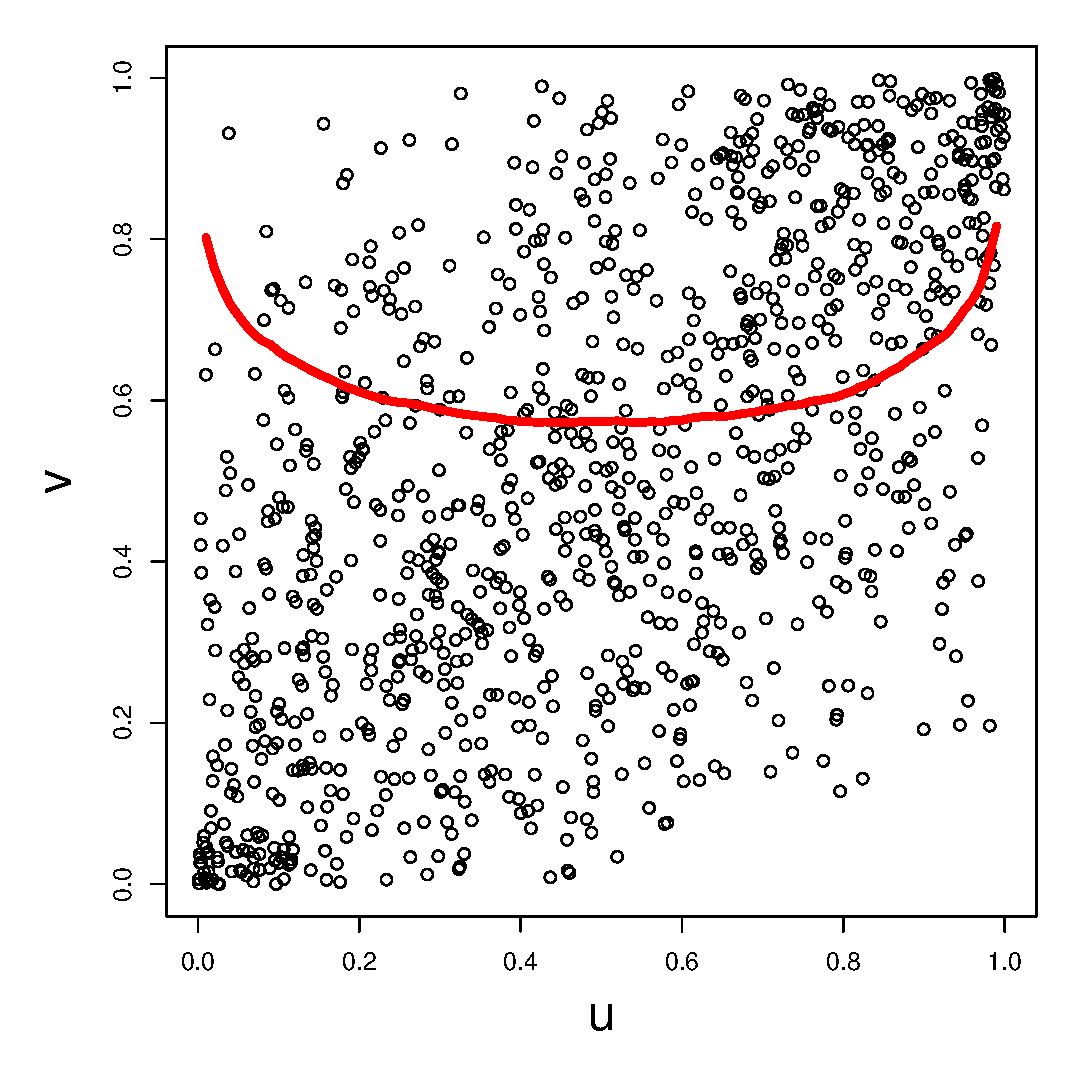
\includegraphics{normal.eps}}
            \resizebox{40mm}{!}{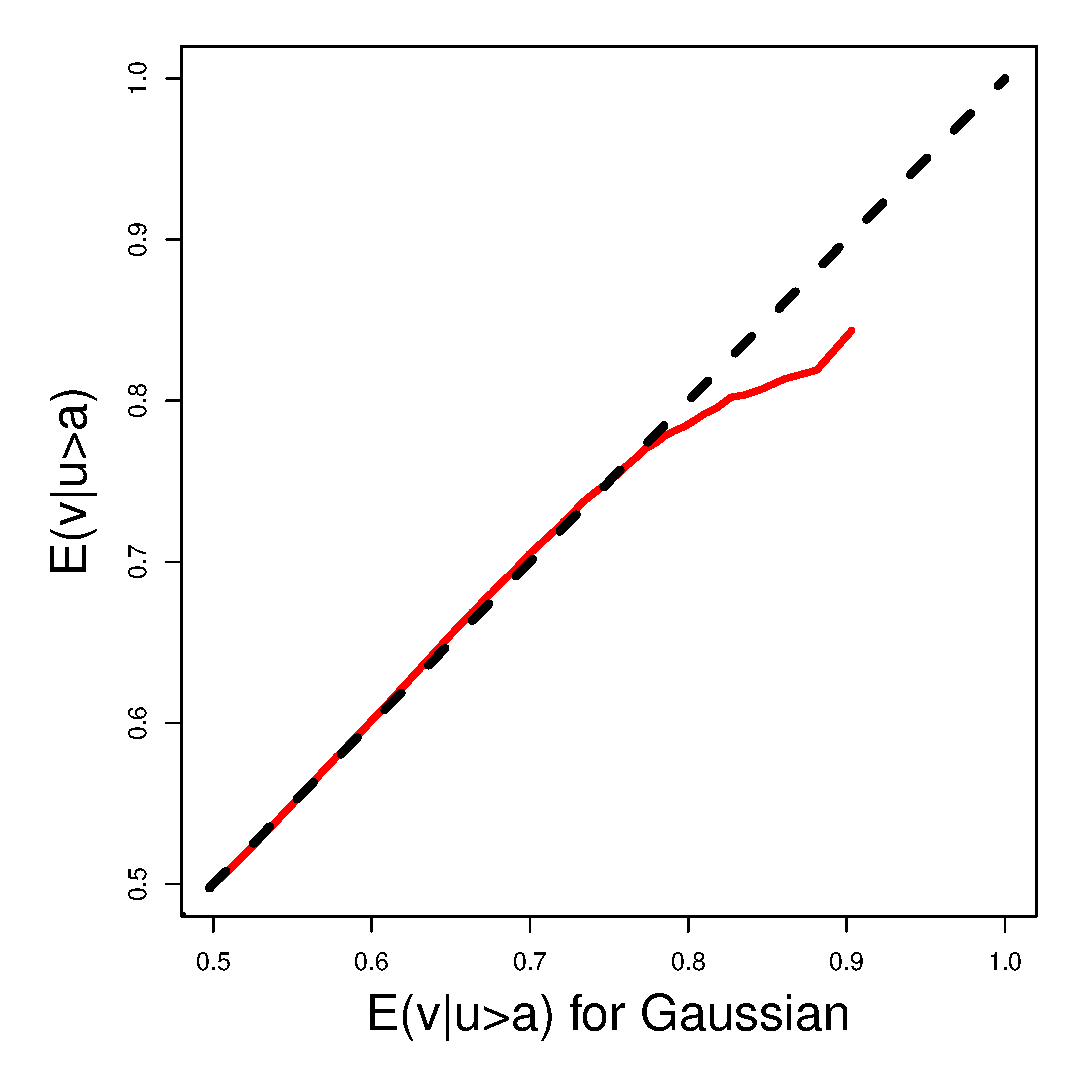
\includegraphics{studentvs.eps}}
      \resizebox{40mm}{!}{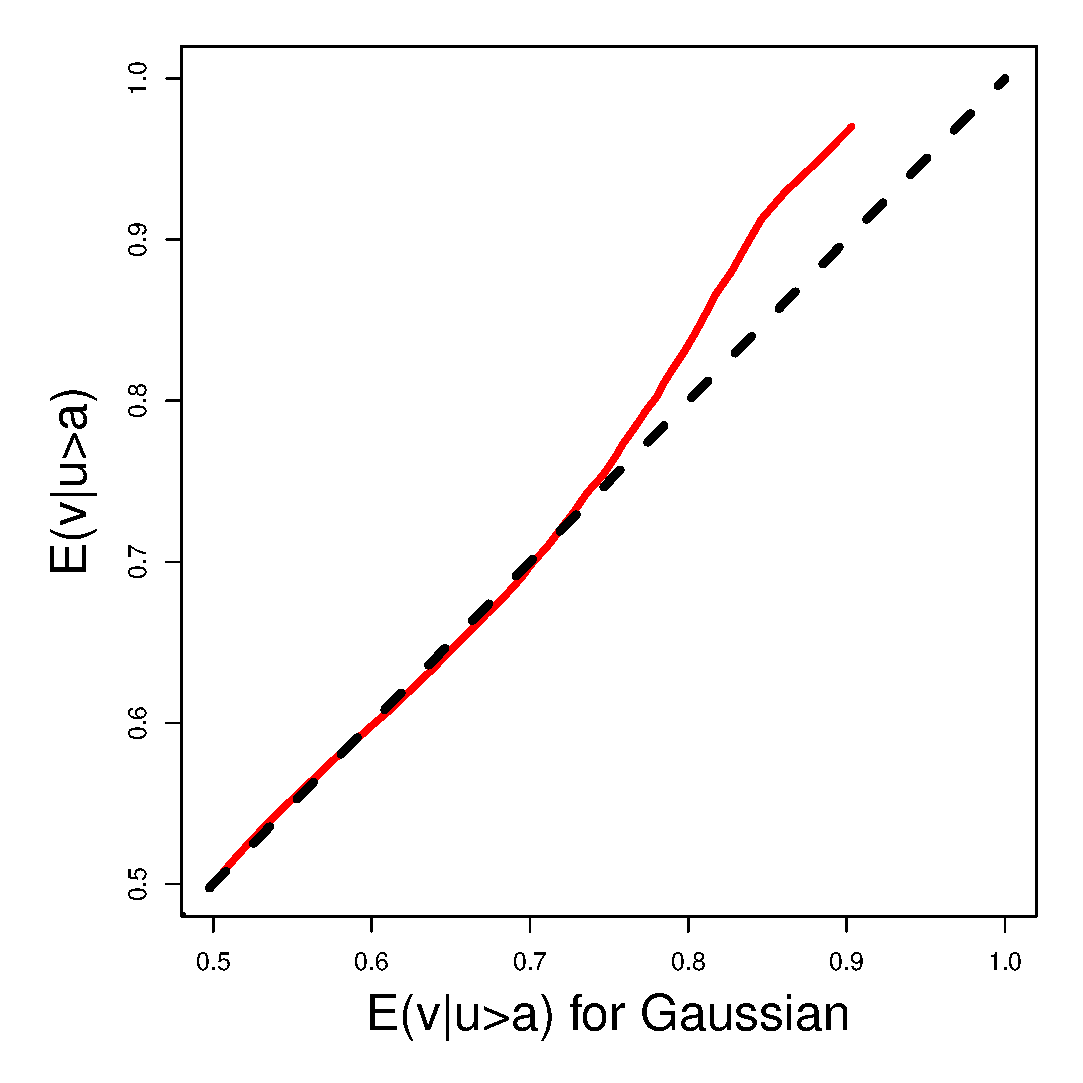
\includegraphics{structural2vs.eps}} \\
      \resizebox{40mm}{!}{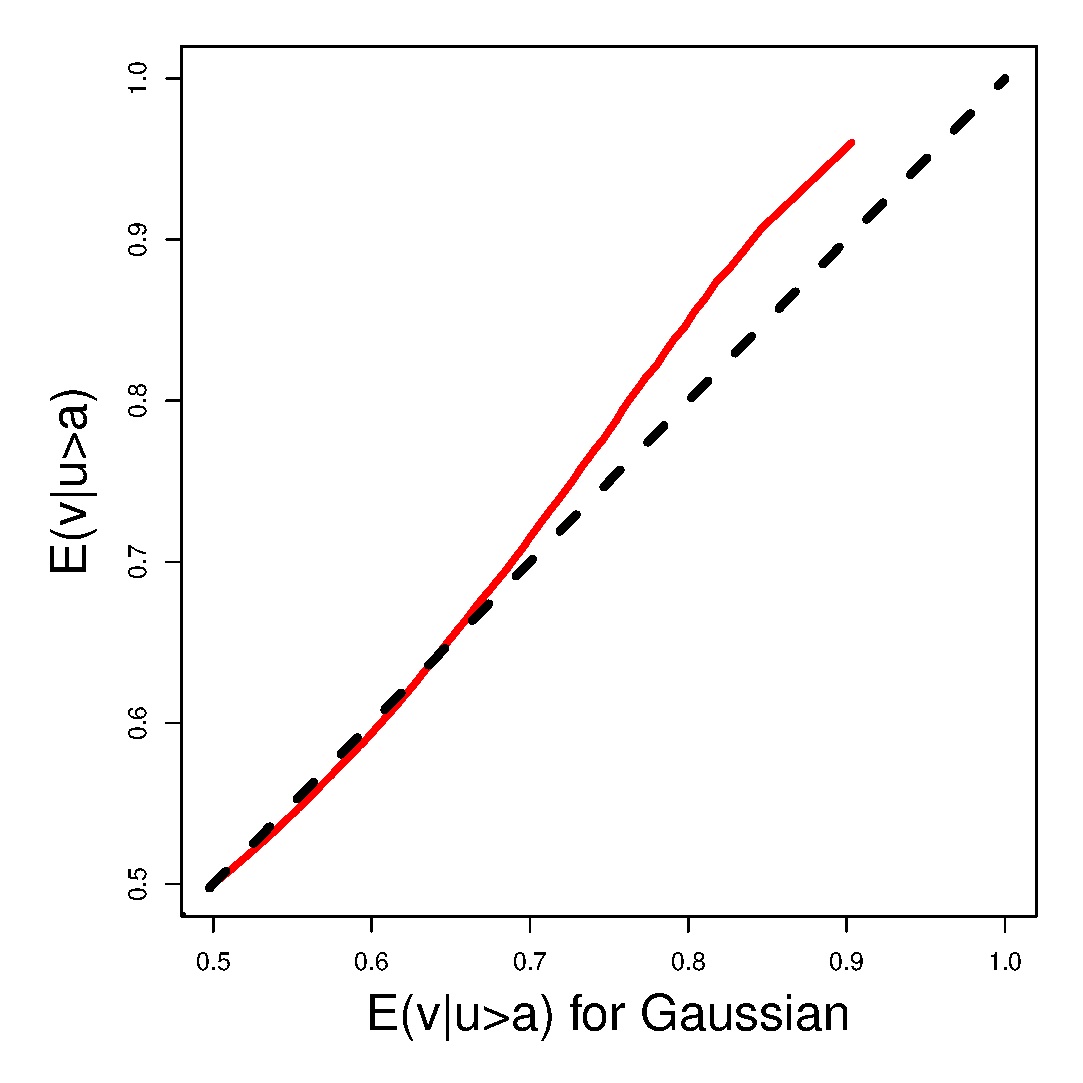
\includegraphics{gumbelvs.eps}}
            \resizebox{40mm}{!}{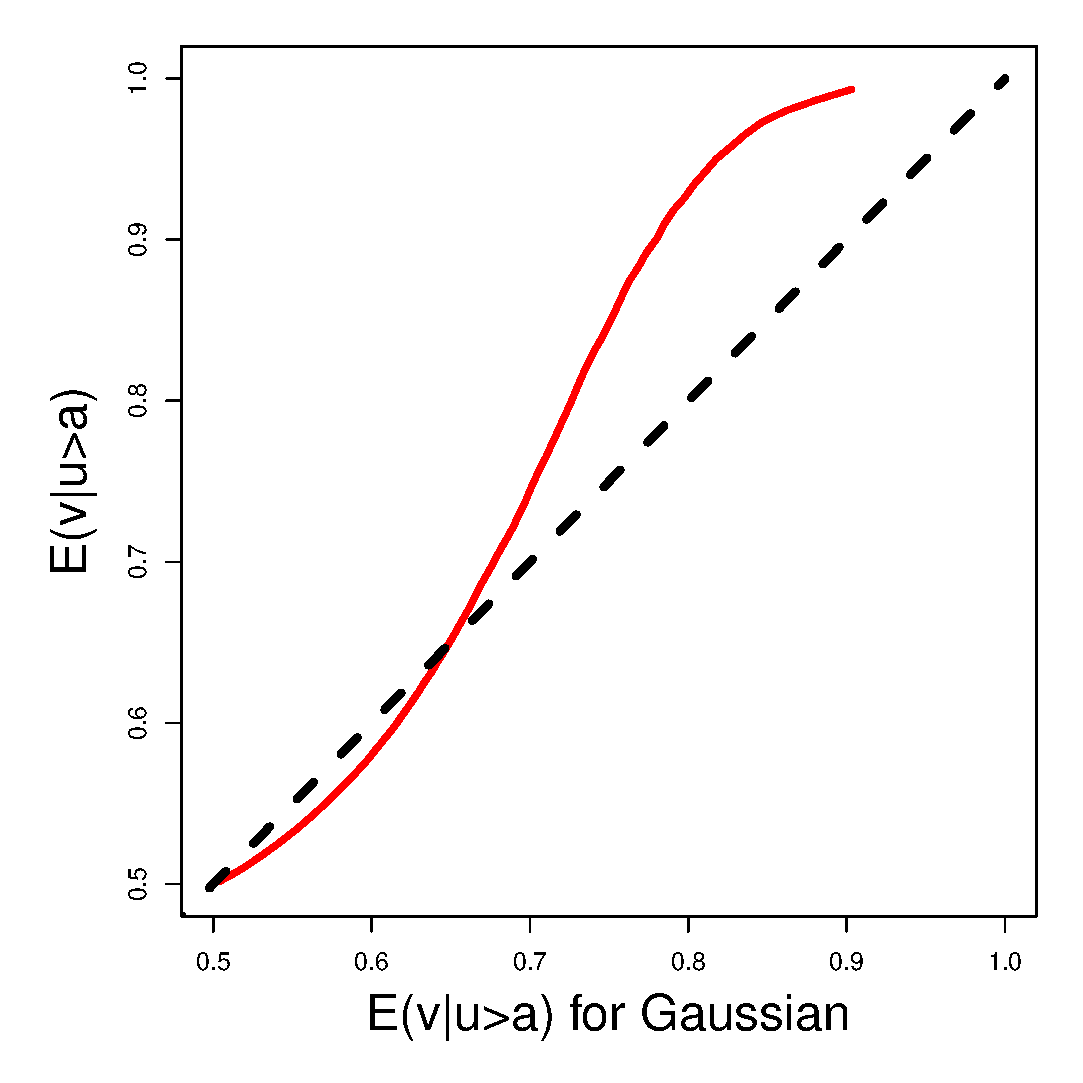
\includegraphics{structural1vs.eps}}
      \resizebox{40mm}{!}{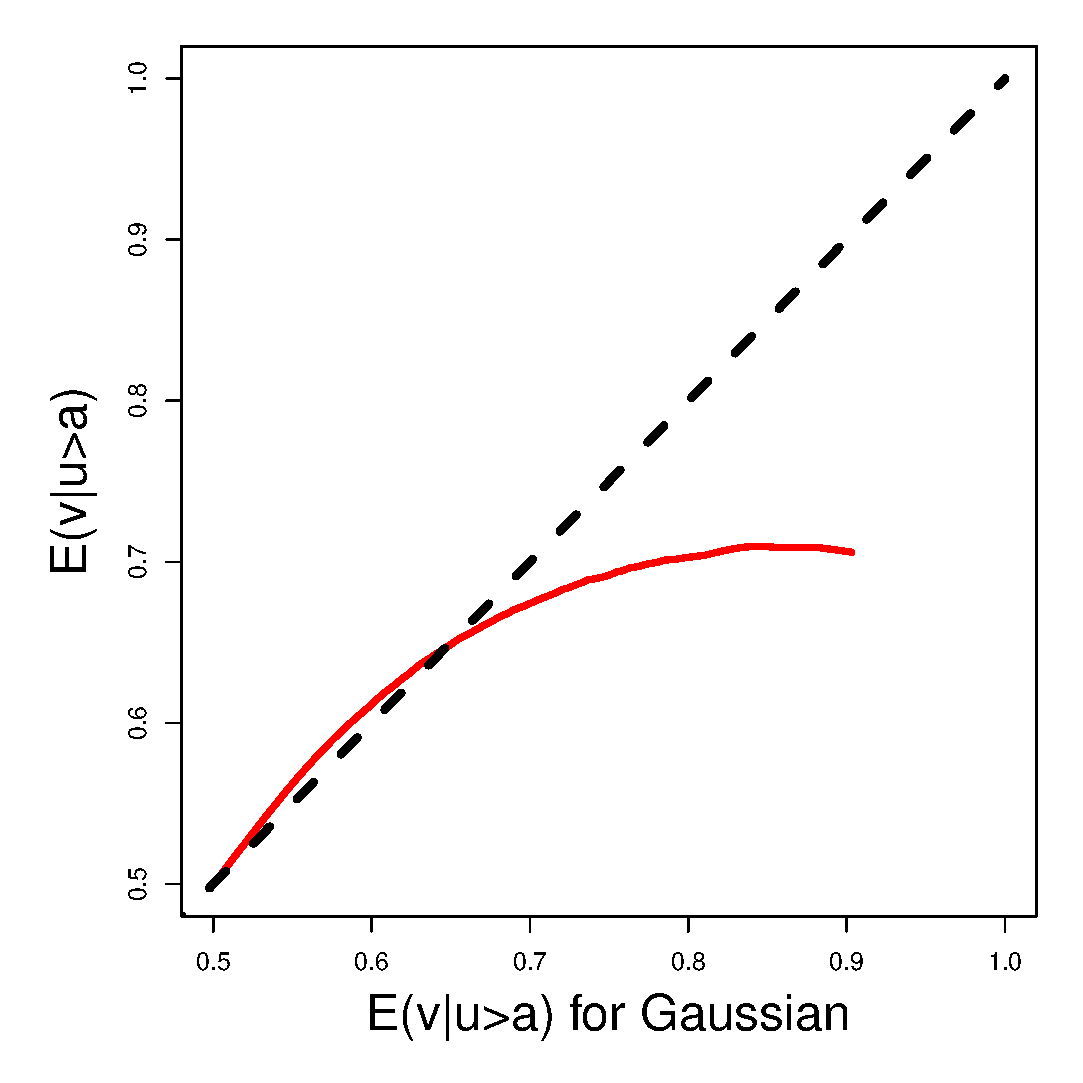
\includegraphics{claytonvs.eps}} \\
            \resizebox{40mm}{!}{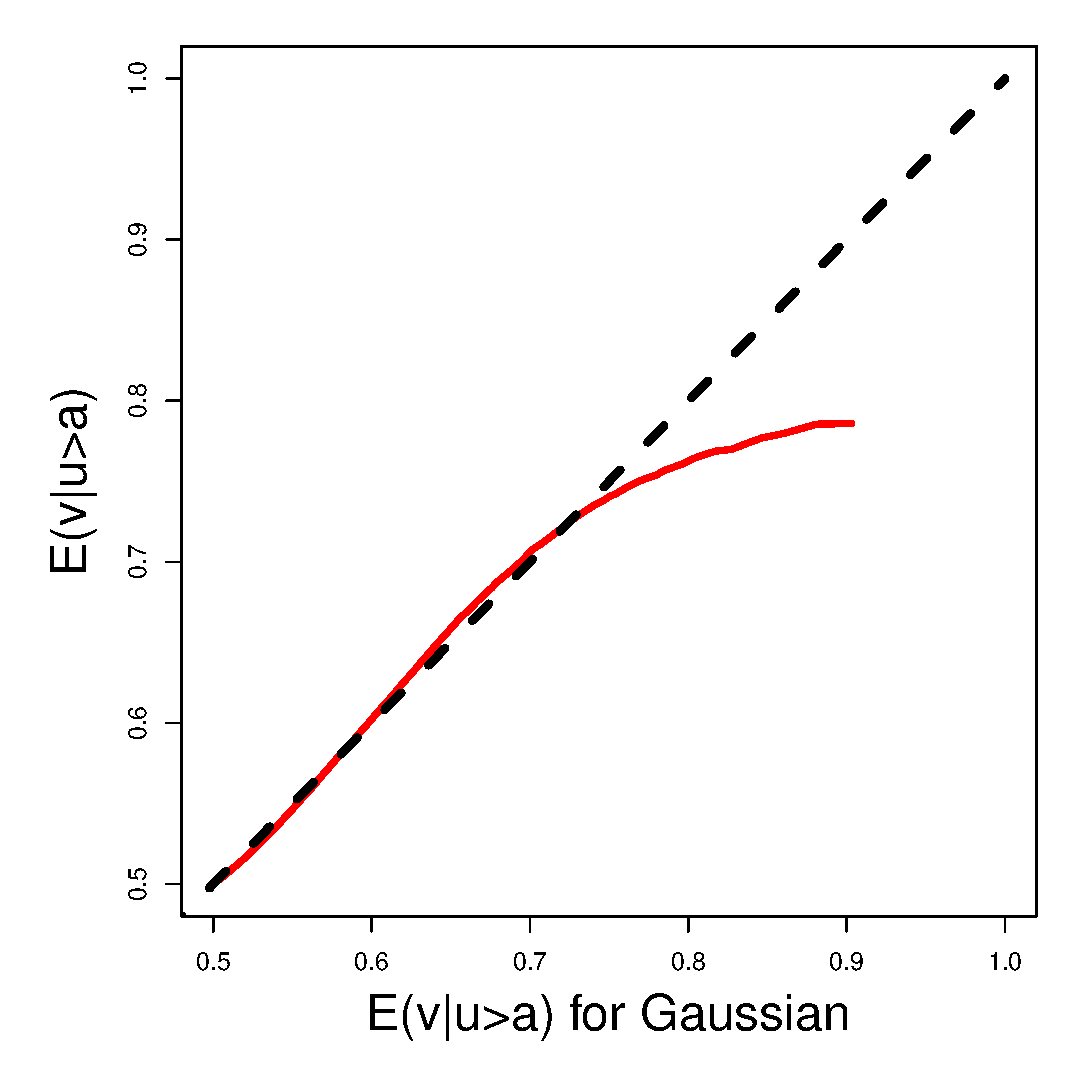
\includegraphics{frankvs.eps}}
            \resizebox{40mm}{!}{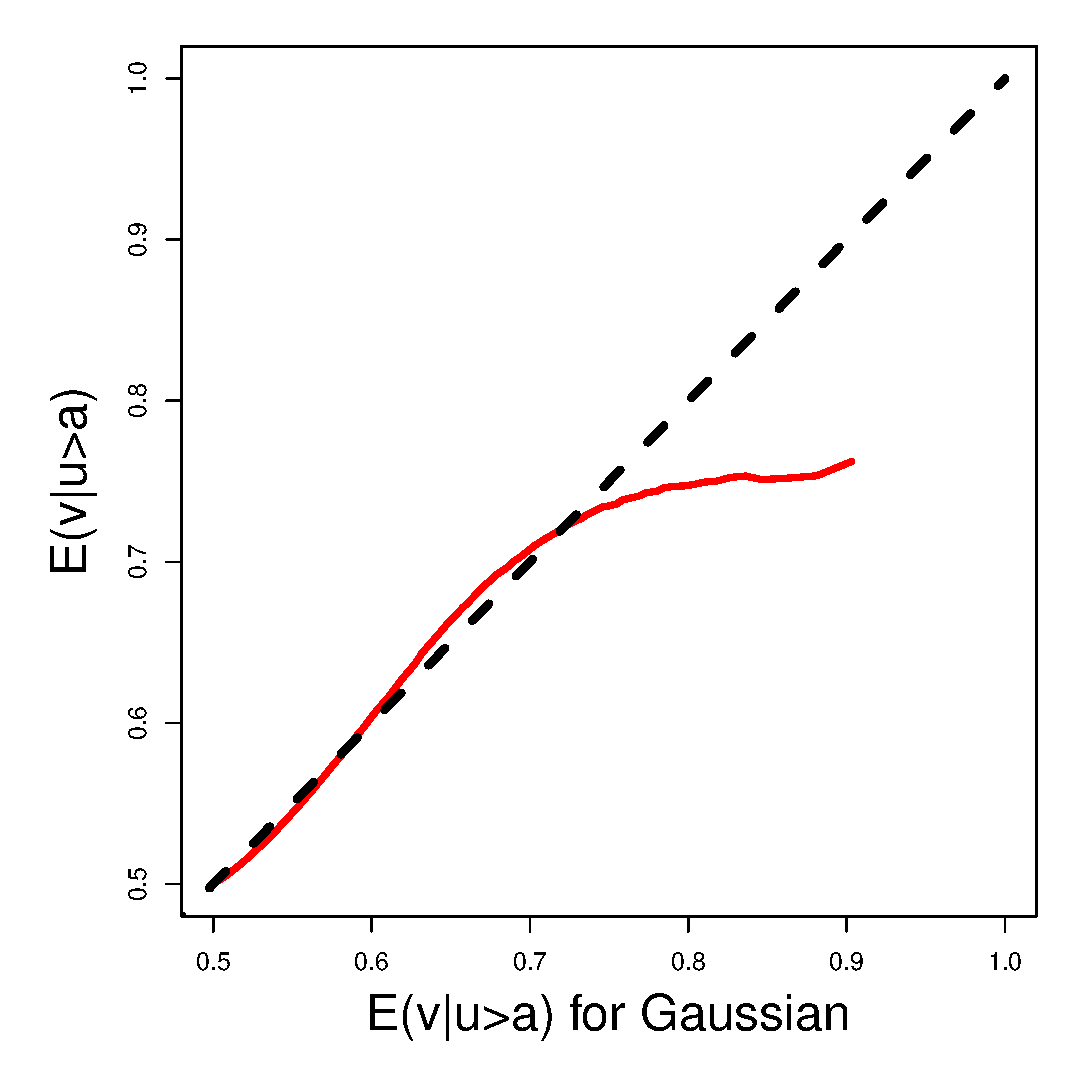
\includegraphics{structural3vs.eps}}
      \resizebox{40mm}{!}{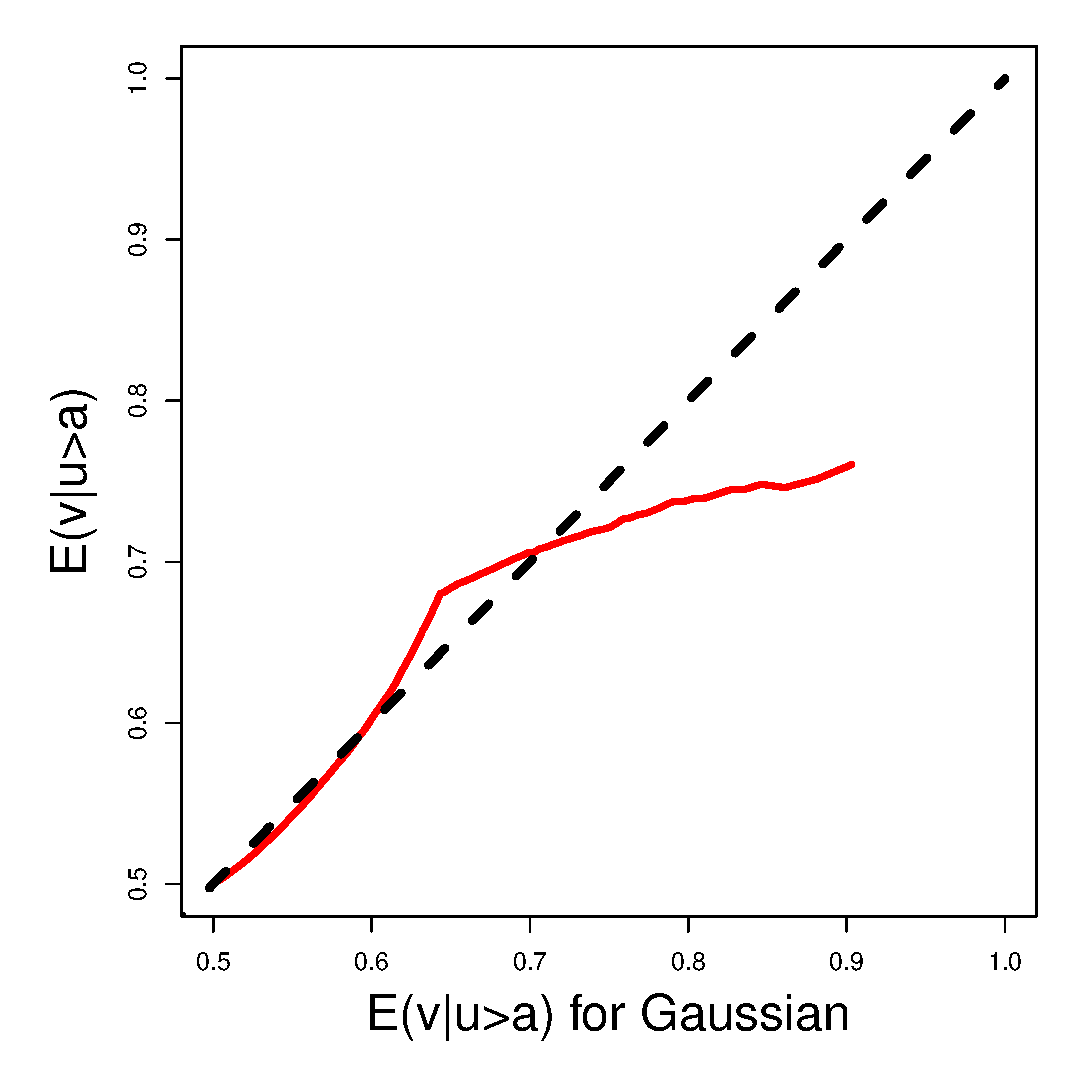
\includegraphics{structural4vs.eps}} \\
    \end{tabular}
    \caption{Plot of upper conditional tail expectations $\E(v|u>\alpha)$ for given copulas against the same for the Gaussian copula.}
    \label{comparison}
  \end{center}
\end{figure}

\fref{fillustration1} expands \fref{fillustration} by graphing layer dependence curves for several parameters of Gaussian, Gumbel, Clayton and Frank copulas. Layer dependence curves summarise essential information (dependence structure) underlying each copula:
\begin{itemize}

\item Gaussian copula: symmetric U-shaped dependence with stronger dependence for larger $\ell$.

\item Gumbel copula: asymmetric U-shaped dependence with stronger dependence for larger $\theta$. Perfect upper tail dependence is always present.

\item Clayton copula: linearly declining dependence with stronger dependence for larger $\theta$. Perfect lower tail dependence is always present.

\item Frank copula: relatively stable dependence with stronger dependence for larger $\theta$.

\end{itemize}
Computing the layer dependence curve is an insightful and important exercise, particularly when the parametric form of a given copula is difficult to interpret, or when the dependence structure underlying an empirical copula is not apparent. Overall dependence measures such as  $\rho_S$ or Kendall's $\tau$ provide information on overall dependence rather than ``local dependence." Section \aref{sliterature} compares layer dependence with existing local dependence measures. It is shown that layer dependence provides a more accurate measure of local dependence. In addition layer dependence possesses coherence properties, further discussed in \sref{scoherence}.

\begin{figure}
  \begin{center}
    \begin{tabular}{cc}
      \resizebox{60mm}{!}{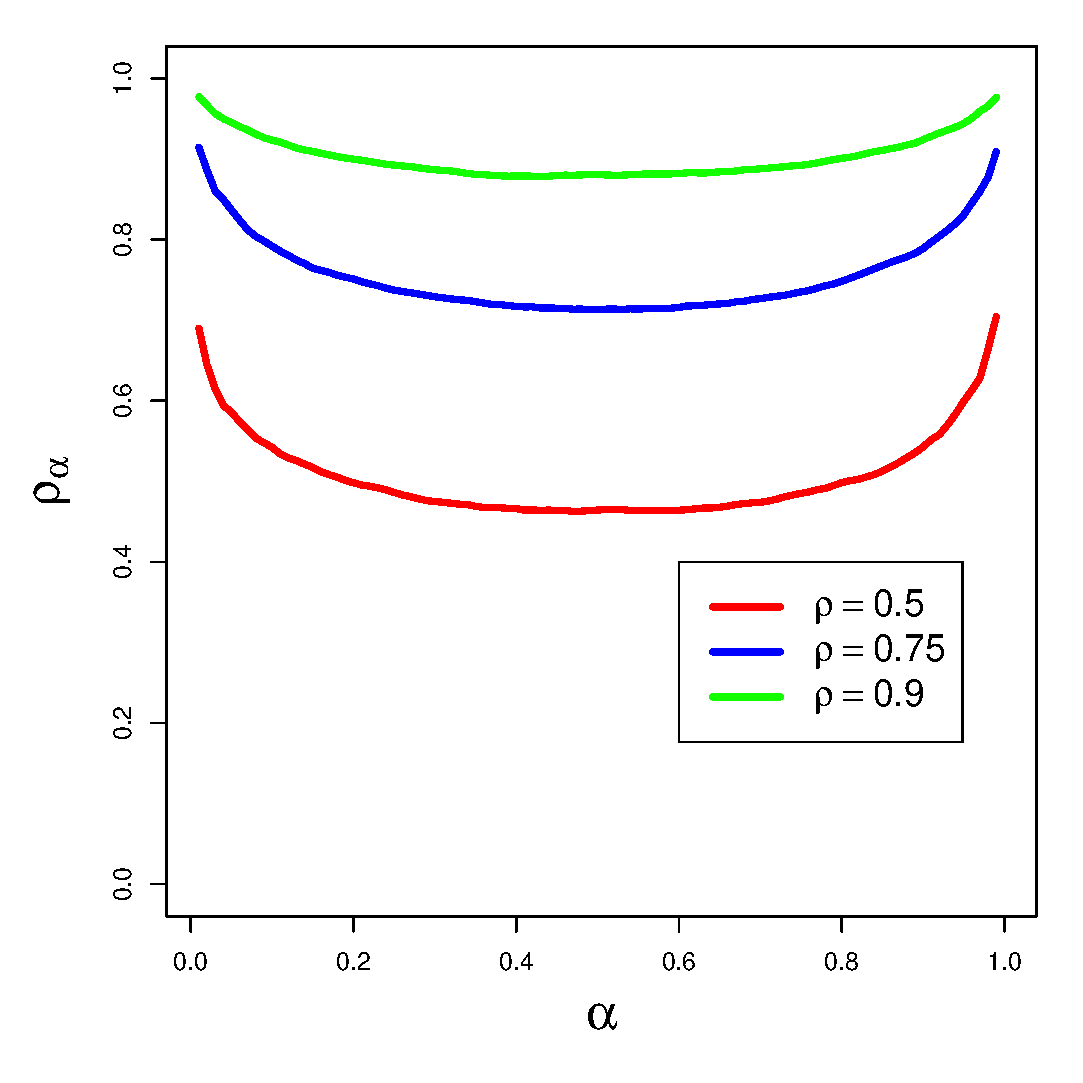
\includegraphics{gaussianmul.eps}}
      \resizebox{60mm}{!}{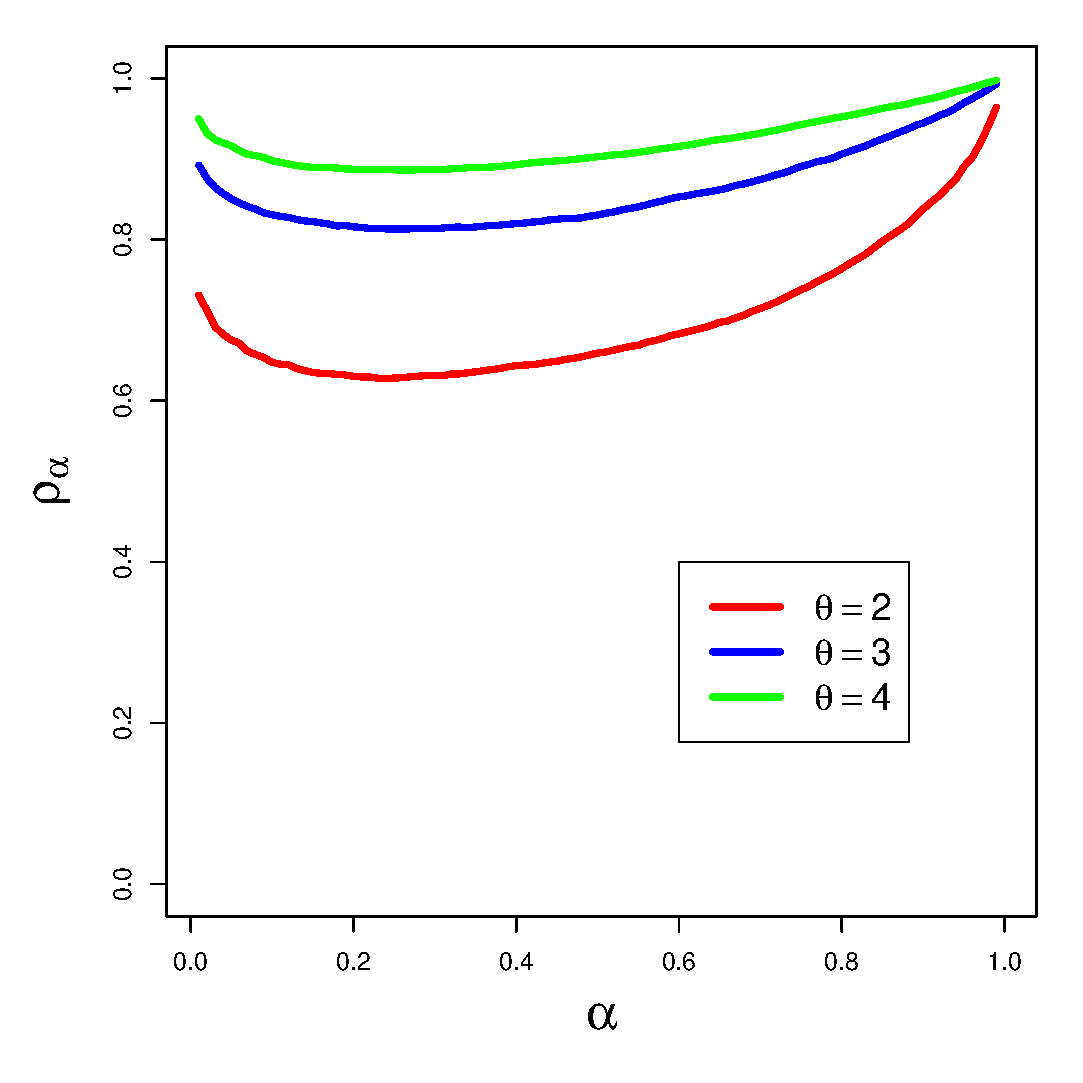
\includegraphics{gumbelmul.eps}} \\
      \resizebox{60mm}{!}{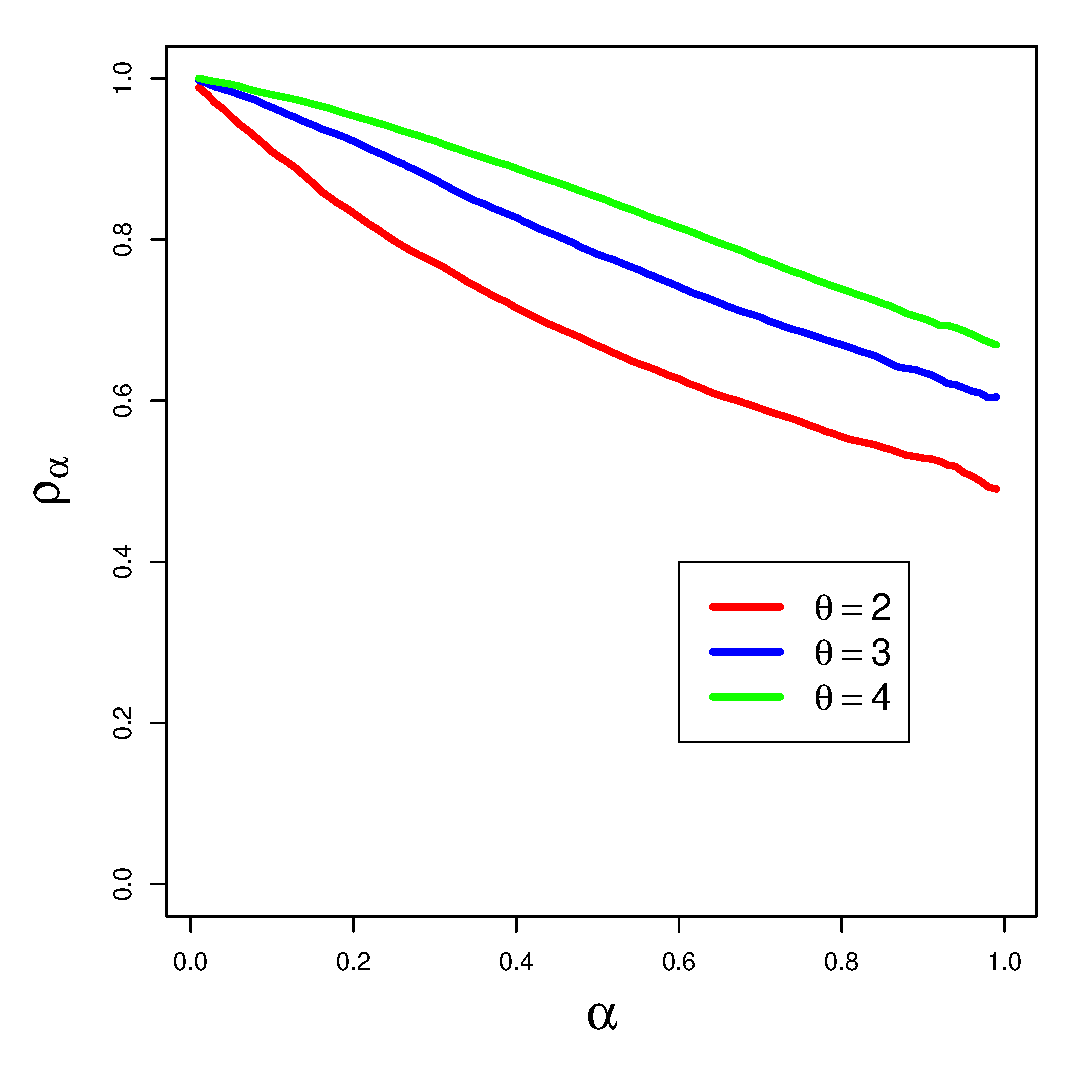
\includegraphics{claytonmul.eps}}
      \resizebox{60mm}{!}{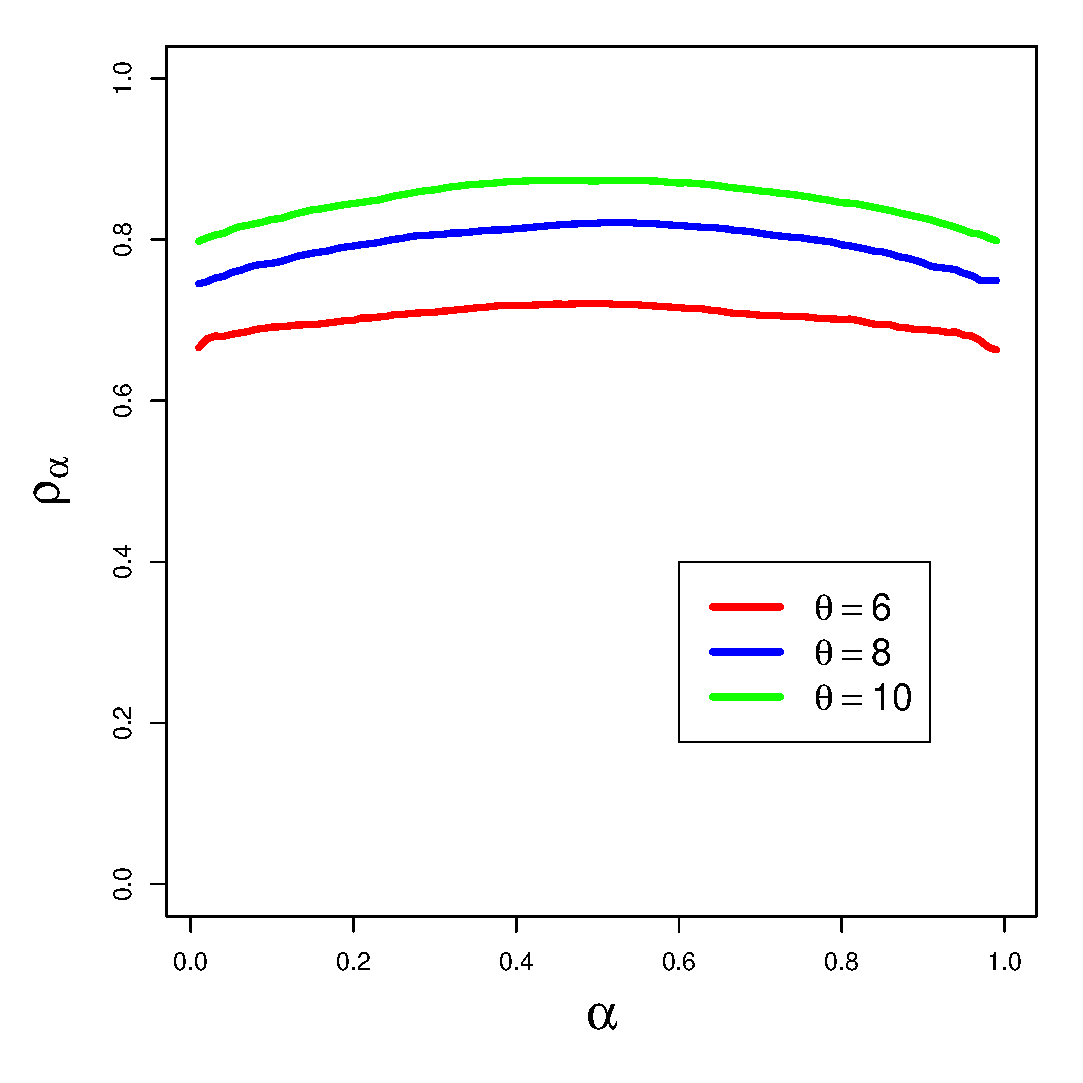
\includegraphics{frankmul.eps}} \\
    \end{tabular}
    \caption{layer dependence curves for various parameters of a Gaussian copula (top left), Gumbel copula (top right), Clayton copula (bottom left) and Frank copula (bottom right). Parameter values are shown in legends.}
    \label{fillustration1}
  \end{center}
\end{figure}





\subsection{``Locality" of layer dependence}

layer dependence $\ell_\alpha$ measures correlation between $u$ in the neighbourhood of $\alpha$ and $v$. This ``locality" property is not apparent from the definition of $\ell_\alpha$. The following is a proof. Define $\ell_{[a,b]}$ as the weighted average
$$
\ell_{[a,b]} \equiv \frac{\int_a^b \ell_\alpha w_\alpha \de \alpha}{\int_a^b w_\alpha \de\alpha}
=\frac{\cov(v,u_{[a,b]})}{\cov(u,u_{[a,b]})}
\cq u_{[a,b]}\equiv \int_a^b (u>\alpha)\de\alpha \;,
$$
where $w_\alpha=6\alpha(1-\alpha)$ and $u_{[a,b]}$ is the ``$[a,b]$ layer" of $u$. Hence the weighted average $\ell_{[a,b]}$ is the scaled correlation between $[a,b]$ layer of $u$ and $v$. Taking the limit $b\rightarrow a^+$ of $\ell_{[a,b]}$ and setting $a=\alpha$ yields $\ell_\alpha$. Rewriting $u_{[a,b]}$ yields
$$
u_{[a,b]}=(u>a)\int_a^{\min(u,b)} \de \alpha = (u>a)\left\{\min(u,b)-a \right\} \;.
$$
Hence the $[a,b]$ layer of $u$ is constant and equal to $0$ when $u\leq a$ and $b-a$ when $u>a$. When $a<u\leq b$, $u_{[a,b]}=u-a$ implying the $[a,b]$ layer of $u$ moves in line with $u$. Therefore the weighted average $\ell_{[a,b]}$ measures correlation between movements of $u$ in the interval $[a,b]$ and $v$. Taking the limit $b\rightarrow a^+$ implies $\ell_\alpha$ measures correlation between $u$ in the neighbourhood of $\alpha$ and $v$. Hence layer dependence measures ``local" dependence.


\subsection{Connection to first-order conditional expectations}

layer dependence in \eref{definition} transforms first order conditional tail expectations into measures of local dependence between $u$ and $v$. Suppose the regression curve of $v$ on $u$, or $\E(v|u=t)$ for all $0\leq t\leq 1$, is given. Then $\alpha$-layer dependence is the integral
$$
\ell_\alpha = 2\left\{\frac{1}{1-\alpha}\int_\alpha^1 \E(v|u=t) \de t - \frac{1}{\alpha}\int_0^\alpha \E(v|u=t) \de t \right\} \;.
$$
Given $\alpha$-layer dependence yields first order conditional expectations:
$$
\E(v|u>\alpha)=\ell_\alpha \E(u|u>\alpha) + 0.5(1-\ell_\alpha)  \;,
$$
$$
\E(v|u=\alpha)=\alpha\ell_\alpha +0.5(1-\ell_\alpha)-0.5\alpha(1-\alpha)\ell'_\alpha \;.
$$
Hence first order conditional expectations are a weighted average of corresponding expectations assuming comonotonicity and independence, with weights $\ell_\alpha$ and $1-\ell_\alpha$, respectively. The conditional expectation $\E(v|u=\alpha)$ requires an additional adjustment term $0.5\alpha(1-\alpha)\ell'_\alpha$ based on the derivative $\ell'_\alpha$.


\end{comment}






\section{Connections to existing measures of tail dependence}\label{sliterature}

Measures have been proposed to capture the degree of tail dependence. Tail dependence is dependence between extreme values of random variables, in this case values of $u$ and $v$ near 0 or 1. Strong tail dependence creates catastrophic events such as  multiple bank failures and  market crashes. Layer dependence is intimately connected to two existing tail dependence measures -- coefficient of tail dependence and tail concentration function. \cite{sweeting2013calculating} and \cite{durante2014copulas} further discuss tail dependence measures.


\subsection{Tail dependence coefficients}

\cite{joe1997multivariate} defines coefficients of lower and upper tail dependence where coefficients of one indicate perfect tail dependence. The following shows that layer dependence characterises perfect tail dependence equivalently as \cite{joe1997multivariate}.

Coefficients of lower and upper positive tail dependence are defined as the limiting conditional tail probabilities
$$
\lambda_L \equiv \lim_{\alpha\rightarrow 0^+} \p(v\leq \alpha |u\leq \alpha) \cq
\lambda_U \equiv \lim_{\alpha\rightarrow 1^-} \p(v>\alpha |u>\alpha) \;.
$$
Unit coefficients indicate perfect positive tail dependence, and occur if and only if $u$ and $v$ converge simultaneously to 0 (lower tail) or 1 (upper tail). Coefficients of negative tail dependence replace $v\leq \alpha$ and $v>\alpha$ in the above expressions with $v>1-\alpha$ and $v\leq 1-\alpha$, respectively.  \cite{sweeting2013calculating} discusses the drawback of these coefficients and suggests a modification by weakening the limits, yielding links to tail concentration functions discussed below.

The following shows $\lambda_L=1$ is equivalent to $\ell_0=1$ and $\lambda_U=1$ is equivalent to $\ell_1=1$. Similar links apply to negative tail dependence. Hence \cite{joe1997multivariate} and layer dependence characterise perfect tail dependence equivalently. From \eref{gapexp}, $\ell_1=2\E(v|u=1)-1$ implying $\ell_1=1$ if and only if $\E(v|u=1)=1$. Hence $\ell_1=1$ if and only if $u=1$ implies $v=1$, which is equivalent to $\lambda_U=1$. In addition $\ell_0=1$ if and only if $u=0$ implies $v=0$, which is equivalent to $\lambda_L=1$. Similar proofs apply to perfect negative tail dependence.



\subsection{Tail concentration function}


Tail concentration \citep{venter2002tails} is a local dependence measure formed from lower and upper conditional tail probabilities. Similar to layer dependence curves, tail concentration functions characterise the dependence structure of copulas and are used to identify families of copulas. The following shows an intimate connection between layer dependence and tail concentration. In addition layer dependence refines tail concentration by incorporating additional information on dispersion defined in \sref{sdecompose}.

The tail concentration function at $\alpha$ is:
$$
\tau_\alpha  \equiv \left\{\begin{array}{cc}\p(v\leq \alpha|u\leq \alpha)\ ,  & \alpha\leq 0.5\ \\
\p(v>\alpha|u>\alpha)\ ,& \alpha>0.5 \ \end{array}\right.
=\left\{\begin{array}{cc}\frac{C(\alpha,\alpha)}{\alpha}\ , & \alpha\leq 0.5\ \\
\frac{1-2\alpha+C(\alpha,\alpha)}{1-\alpha}\ ,& \alpha>0.5 \ \end{array}\right. \;.
$$
Higher $\tau_\alpha$ implies $u$ and $v$ are more likely to fall in the same tail -- lower tail if $\alpha\leq 0.5$ and upper tail if $\alpha>0.5$. In addition taking limits $\alpha\rightarrow 0$ and $\alpha\rightarrow 1$ of $\tau_\alpha$ yield coefficients of tail dependence $\lambda_L$ and $\lambda_U$ discussed above. Properties of tail concentration and its applications to distinguish families of copulas are further discussed in \cite{durante2014copulas}.


To show the connection between layer dependence and tail concentration, first standardise $\tau_\alpha$ by subtracting its value under independence and dividing by the difference between $\tau_\alpha$ under comonotonicity and independence:
$$
\tau_\alpha^*=\frac{\tau_\alpha-\tau_\alpha^0}{\tau_\alpha^+-\tau_\alpha^0} = \frac{C(\alpha,\alpha)-\alpha^2}{\alpha(1-\alpha)}
$$
where $\tau_\alpha^0=\tau_\alpha$ if $u$ and $v$ are independent and $\tau_\alpha^+=\tau_\alpha$ if $u=v$, hence
$$
\tau_\alpha^0=\left\{\begin{array}{cc}\alpha \ , & \alpha\leq 0.5\ \\
1-\alpha \ ,& \alpha>0.5 \ \end{array}\right.
\cq
\tau_\alpha^+=1 \;.
$$
Standardised tail concentration $\tau_\alpha^*$ is 1 if $u=v$ and $0$ if $u$ and $v$ are independent. 

Note the final expression for $\tau_\alpha^*=-\gamma_\alpha$ where $\gamma_\alpha$ measures discordance between $u$ and $v$ at $\alpha$ as discussed in \sref{sdecompose}. Combining this result with \eref{decompose} yields
$$
\ell_\alpha=1-2\delta_\alpha(1-\tau_\alpha^*) = 1-2\delta_\alpha + 2\delta_\alpha \tau_\alpha^*
$$
where $\delta_\alpha$ as defined in \sref{sdecompose} measures average dispersion between discordant $u$ and $v$ at $\alpha$. Hence given $\alpha$, $\ell_\alpha$ is increasing in $\tau_\alpha^*$ and $\tau_\alpha$. It is also straightforward to show that $\ell_\alpha=1$ is equivalent to $\tau_\alpha^*=1$.

Hence there is an intimate connection between tail concentration and layer dependence. However tail concentration (in its standardised form) is only one of two factors forming layer dependence. The other factor is the dispersion between discordant points, measured by $\delta_\alpha$. Using the right panel of \fref{finterpretation}, $\tau_\alpha$ or $\tau_\alpha^*$ only reflects the number of discordant points at $\alpha$, whereas layer dependence combines this information and average dispersion between discordant points. Hence layer dependence refines tail concentration in two ways: first by standardising and then including further information on dispersion.





\section{Further properties of layer dependence}\label{sproperties}

This section lists and explores further properties and results of layer dependence.




\subsection{Copula integration}

Layer dependence $\ell_\alpha$ can be written as a standardised integral of the copula:
\begin{equation}\label{copula}
\ell_\alpha = \frac{\int_0^1 \cov\{I_\alpha(u),I_\beta(v)\} \de\beta }{\alpha(1-\alpha)/2}
= \frac{2 \int_0^1 C(\alpha,\beta) \de \beta- \alpha}{\alpha(1-\alpha)} \;.
\end{equation}
The result follows from \eref{ellalpha} by decomposing $v=\int_0^1 I_\beta(v)\de v$ similar to \eref{decompose} and noting $\cov\{I_\alpha(u),I_\beta(v)\}=C(\alpha,\beta)-\alpha\beta$.

Thus $\ell_\alpha$ integrates copulas to reduce their dimension from two and one, and scales the result to ensure it lies between $\pm 1$. This computation extracts the dependence structure from the copula. In comparison, tail concentration performs the dependence extraction by computing the diagonal section $C(\alpha,\alpha)$.

\begin{comment}
With Archimedean copulas \citep{mcneil2005qrm} $C(\alpha,\beta) =\psi^-\left\{\psi(\alpha)+\psi(\beta)\right\}$ where $\psi$ is the generator function and $\psi^-$ its inverse. In this case closed form expressions for the integrals and hence for $\ell_\alpha$ do not exist.
\end{comment}


\subsection{Layer dependence preserves convex combination}

A direct consequence of the copula integration result \eref{copula} is layer dependence preserves convex combinations of random variables, as follows.

Suppose $(u^*,v^*)$ is bivariate uniform with $\alpha$--layer dependence $\ell_\alpha^*$ and copula $C^*$. Then a mixture of $(u,v)$ and $(u^*,v^*)$ yielding the copula $\pi C+(1-\pi)C^*$ where $0\le \pi\le 1$ has layer dependence $\pi\ell_\alpha+(1-\pi)\ell_\alpha^*$. Hence layer dependence preserves convex combinations of copulas. The proof follows directly from \eref{copula}.

It is also straightforward to show that layer dependence preserves multiple and continuous convex combinations of copulas.



\subsection{One-sided conditional tail expectations}


Since $\E(v)=\alpha\E(v|u\leq \alpha)+(1-\alpha)\E(v|u>\alpha)$ it is straightforward to show from \eref{gapexp} that
$$
\ell_\alpha = \frac{\E(v|u> \alpha)-\E(v)}{\E(u|u> \alpha)-\E(u)} = \frac{\E(v|u\leq \alpha)-\E(v)}{\E(u|u\leq \alpha)-\E(u)} \;,
$$
the gap between upper or lower conditional tail expectations of $v$ and the unconditional expectation. Denominators are again scaling factors ensuring $\ell_\alpha=1$ if $u$ and $v$ are comonotonic and $\ell_\alpha=-1$ if countermonotonic.

\begin{comment}
Rewriting conditional tail expectations in \eref{gapexp} in terms of ``pointwise" conditional expectations yields
$$
\ell_\alpha = 2\left\{\frac{1}{1-\alpha}\int_\alpha^1 \E(v|u=t) \de t - \frac{1}{\alpha}\int_0^\alpha \E(v|u=t) \de t \right\} \;,
$$
hence $\alpha$-layer dependence is the difference between average points on the regression curve of $v$ on $u$ over $u>\alpha$ and $u\leq\alpha$.
\end{comment}



\subsection{Layer dependence does not uniquely characterise a copula}


Layer dependence curves extract and summarise dependence information from a copula. Therefore layer dependence curves do not uniquely specify the copula, as shown in the following counterexample.

Suppose $v=u$ and $v=1-u$ with equal probability. The former and latter imply $\ell_\alpha=1$ and $-1$, respectively, for all $\alpha$. Hence $\ell_\alpha=0$ since layer dependence preserves convex combinations as discussed above. The copula of $(u,v)$ is $C(u,v)=0.5\{\min(u,v)+\max(u+v-1,0)\}$. However $\ell_\alpha=0$ is also the case for independent $u$ and $v$: $C(u,v)=uv$. Hence layer dependence curves are not unique to the copula.

Non-uniqueness is seen from another perspective using \eref{gapexp}: $\ell_\alpha$ only captures first-order conditional tail expectations. Hence two copulas with equal first-order conditional tail expectations have equal layer dependence.

\begin{comment}

\subsection{Non-exchangeability}

layer dependence retains coherence and dependence-measuring properties when the joint distribution of $(u,v)$ is non-exchangeable. However the calculation of layer dependence differs according to the conditioning variable:
$$
2\left\{\E(v|u>\alpha)-\E(v|u\leq \alpha)\right\} \neq
2\left\{\E(u|v>\alpha)-\E(u|v\leq \alpha)\right\} \;.
$$
The left expression measures local dependence with respect to $u$. The right expression measures local dependence with respect to $v$, and is not necessarily equal to the left. A similar concept applies in regression, where the regression coefficient depends on the assignment of explanatory and dependent variables.

\end{comment}




\subsection{Layer dependence for a non-exchangeable copula}

If the copula of $u$ and $v$ is not exchangeable, $C(u,v)\neq C(v,u)$, then layer dependence changes when $v$ is decomposed into layers rather than $u$:
$$
\frac{\cov\{v,I_\alpha(u)\}}{\cov\{u,I_\alpha(u)\}}
\neq \frac{\cov\{u,I_\alpha(v)\}}{\cov\{v,I_\alpha(v)\}}  \;,
$$
that is, the dependence between $v$ and $\alpha$--layer of $u$ differs from the dependence between $u$ and $\alpha$--layer of $v$.

An analogous property applies to least squares regression: regressing $v$ on $u$ is different from regressing $u$ on $v$ if the joint distribution is not exchangeable. 








\section{Alternate measures of overall dependence}\label{saltoverall}


For various reasons it may still be necessary to refer to measures of overall dependence such as Spearman's correlation. However as discussed in \sref{sintroduction}, Spearman's correlation dismisses tail dependence and may be a less appropriate measure when tail dependence is important such as in insurance and finance. The following formulates alternative measures of overall dependence by taking different weighted averages of layer dependence.


Equation \eref{wtdavg} expresses Spearman's correlation as a weighted average of $\ell_\alpha$ over $0\le\alpha\le 1$ using weights $w_\alpha=6\alpha(1-\alpha)$ integrating to 1. Averaging $\ell_\alpha$ using different weights $w^*_\alpha$ yields alternate measures of overall rank dependence:
$$
\rho^*\equiv  \int_0^1 w^*_\alpha \ell_\alpha \de \alpha 
= \int_0^1 w^*_\alpha \frac{ \cov\{v,I_\alpha(u)\}}{\cov\{u,I_\alpha(u)\}} \de \alpha=\cov\{v,W^*(u)\} \;,
$$
where the final expression follows by bringing the integral into the covariance calculation and
$$
W^*(u)\equiv \int_0^1 \frac{w^*_\alpha I_\alpha(u)}{\cov\{u,I_\alpha(u)\}}\de\alpha  
= 2\int_0^u \frac{w^*_\alpha }{\alpha(1-\alpha)}\de\alpha  
\cq \int_0^1 w_\alpha^* \de\alpha=1 \;.
$$
$W^*$ is the weighted cumulative of $w^*_\alpha$ and $w_\alpha^*$ indicates the weight or importance of local dependence at $\alpha$--layer of $u$. 

Hence the alternate overall dependence measure $\rho^*$ is also a covariance, between $v$ and a transformation of $u$. For Spearman's correlation $\rho$, $w^*_\alpha=6\alpha(1-\alpha)$ thus $W^*(u)=12u$ yielding $\rho^*=\cov(12u,v)=\cor(u,v)=\rho$. Note that even though the expression for $\rho^*$ is asymmetric in $u$ and $v$, the result is identical when $u$ and $v$ are switched if the copula $C$ is exchangeable.

Since $\rho^*$ averages $\ell_\alpha$ using non-negative weights which integrate to 1, all coherence properties of $\ell_\alpha$ described in \sref{scoherence} apply to $\rho^*$. Specifically $-1\le\rho^*\le 1$, $\rho^*=-1$, $0$ and $1$ under countermonotonicity, independence and comonotonicity, respectively, $\rho^*$ switching its sign when $u$ or $v$ is replaced by its complement, and higher $\rho^*$ when the correlation order of $(u,v)$ increases. Identical properties apply to Spearman's correlation.


The following are examples of $w_\alpha^*$ yielding alternate rank dependence measures $\rho^*$:
\begin{itemize}

\item Suppose dependence at different percentiles are equally important. Then $w^*_\alpha=1$ yielding the alternate overall dependence measure
$$
\rho^*_1 =2\cov\left\{v,\log\left(\frac{u}{1-u}\right)\right\}
= \frac{\pi}{3}\ \cor\left\{v,\log\left(\frac{u}{1-u}\right)\right\} \;,
$$
\begin{comment}
\int_0^1 \frac{\cov\{v,(u>\alpha)\}}{\cov\{u,(u>\alpha)\}} \de \alpha
=\cov\left[v,\int_0^1 \frac{(u>\alpha)}{\cov\{u,(u>\alpha)\} }\de \alpha\right]
$$
$$
=\cov\left\{v,\int_0^u \frac{1}{0.5\alpha(1-\alpha) }\de \alpha\right\}
\end{comment}
a multiple of correlation between $v$ and the logit of $u$. The final expression follows by noting $v$ and $\log\{u/(1-u)\}$ have standard deviations $1/\sqrt{12}$ and $\pi/\sqrt{3}$, respectively. If tail dependence is pronounced, $\rho_1^*>\rho$ since $\rho^*_1$ weights tail dependence more heavily compared to $\rho$. An illustration $\rho_1^*$ and other alternates to $\rho$ is shown below.

\item If $w^*_\alpha=3\alpha^2$  then dependence at higher percentiles are considered more important. This formulation is applicable when upper tail dependence is critical, for example the simultaneous occurrence of large insurance losses in different lines of business. Then
$$
\rho_2^* = 6\cov\left\{v,\log\left(\frac{\e^{-u}}{1-u}\right) \right\}
=\sqrt{3} \cor\left\{v,-\log(1-u)\right\}-\frac{\rho}{2}\;,
$$
noting $-\log(1-u)$ has standard deviation 1. This dependence measure combines $\rho$ and the correlation between $v$ and logarithmic transform of $u$. If dependence is higher above the median then $\rho_2^*>\rho$.

\item If dependence over percentiles below the median is more important then for example  $w^*_\alpha=3(1-\alpha)^2$ yielding
$$
\rho_3^* = 6\cov\left\{v,\log \left( u \e^{-u}\right) \right\}
= \sqrt{3}\cor(v,\log u )-\frac{\rho}{2}  \;,
$$
similar to $\rho_2^*$ with an opposite logarithmic transform on $u$.

\item Suppose $w^*_\alpha$ is derived from $V_\alpha$, representing the inverse distribution of $x$ with derivative $V_\alpha'$:
$$
w^*_\alpha = \frac{\cov\{u,I_\alpha(u)\}V_\alpha'}{\int_0^1 \cov\{u,I_\alpha(u)\}V_\alpha' \de\alpha}
=\frac{0.5\alpha(1-\alpha)V_\alpha'}{\cov(u,V_u)}
=\frac{0.5\alpha(1-\alpha)V_\alpha'}{\cov(u,x)} \;,
$$
where $\int_0^1 I_\alpha(u)V_\alpha'\de\alpha=\int_0^u V_\alpha'\de\alpha=V_u$ and $x=V_u$. This weight formulation yields the Gini correlation  \citep{schechtman1999proper}
$$
\rho_4^*=\frac{\cov(v,V_u)}{\cov(u,V_u)} = \frac{\cov\{G(y),x\}}{\cov\{F(x),x\}} \;,
$$
where $F\equiv V^-$ and $G$ are distribution functions of observed random variables $x$ and $y$ with percentile ranks $u$ and $v$, respectively.  In this example the weights $w^*_\alpha$ depend on the marginal distribution of $x$. More skewness in $x$ leads to more steeply increasing $V_\alpha'$ and  $w^*_\alpha$ hence greater emphasis on upper tail dependence.

\end{itemize}

\fref{falternate} illustrates the first three alternates to Spearman's correlation listed above using a Clayton copula shown in \fref{fillustration}. Note $\rho$, $\rho_1^*$, $\rho_2^*$ and $\rho_3^*$ are all weighted averages of $\ell_\alpha$. However their values differ depending on the weight function used. As the Clayton copula exhibits lower tail dependence, $\ell_\alpha$ is decreasing in $\alpha$. Hence $\rho_1^*>\rho$ as $\rho_1^*$ places relatively higher weight on large values of $\ell_\alpha$ in the lower tail. $\rho_3^*$ is the largest as it places the most weight on the lower tail, whereas $\rho_2^*$ is the smallest as it focusses on upper tail dependence. Hence $\rho_3^*$ is a sensitive measure of lower tail dependence and is appropriate when lower tail dependence is of main concern, and vice versa for $\rho_2^*$.

\begin{figure}
  \begin{center}
    \begin{tabular}{cc}
      \resizebox{60mm}{!}{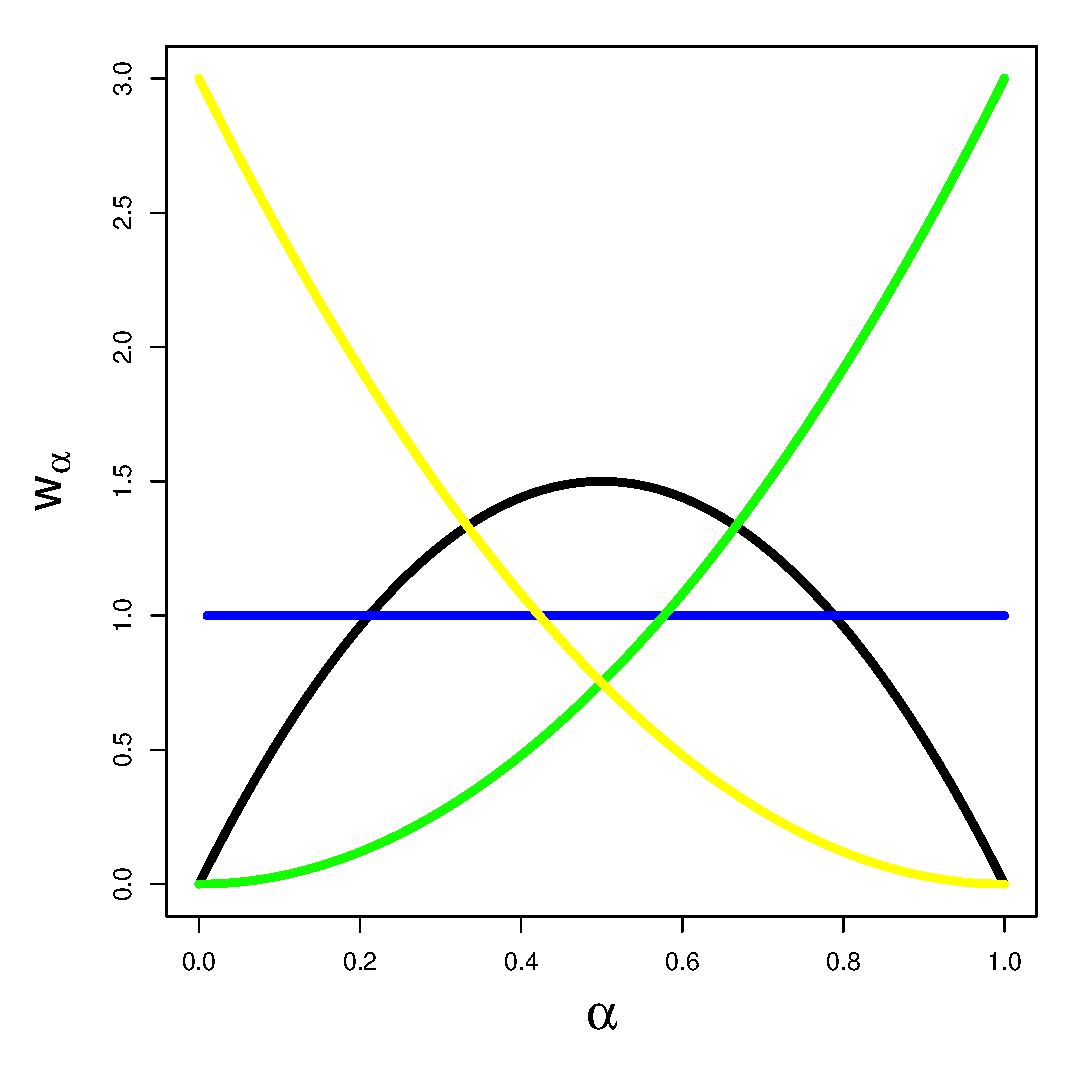
\includegraphics{weights.eps}}
      \resizebox{60mm}{!}{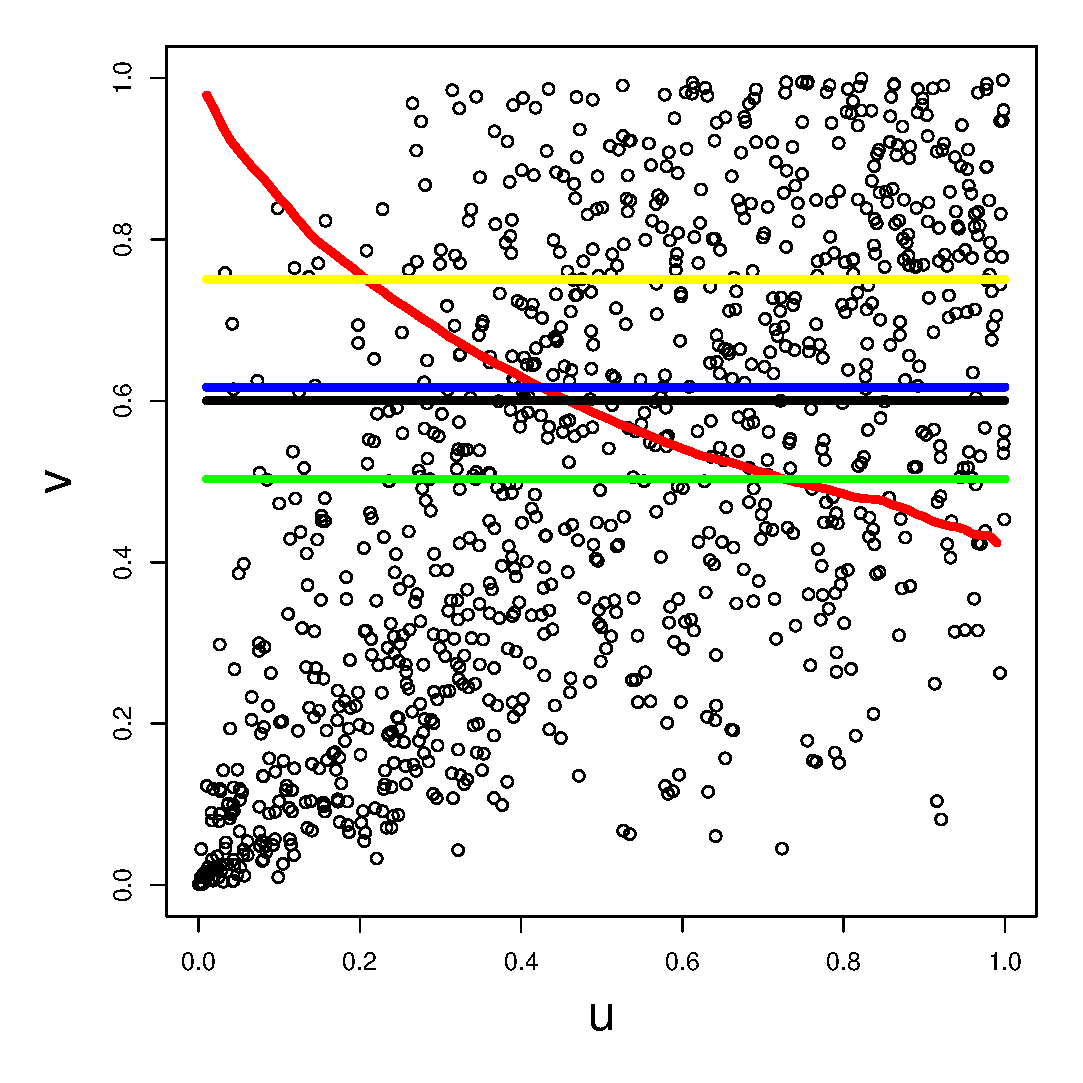
\includegraphics{alternate.eps}} \\
    \end{tabular}
    \caption{The left panel shows the weight functions $w_\alpha=6\alpha(1-\alpha)$ (black), $w_\alpha^*=1$ (blue), $w_\alpha=3\alpha^2$ (green), $w_\alpha=3(1-\alpha)^2$ (yellow). The right panel shows a Clayton copula with a red layer dependence curve and overall dependence measures $\rho$ and $\rho^*$ indicated using the same colors as the left panel.  }
    \label{falternate}
  \end{center}
\end{figure}




\section{Discussion of copula fitting involving layer dependence}\label{sfitting}


This section discusses how layer dependence can be applied to select and fit copulas using past data and expert judgement.

The literature discusses copula fitting extensively. A common approach is to first select parametric copula and marginal distributions, then estimate parameters by maximising joint likelihood \citep{denuitactuarial}. A semi-parametric approach replaces marginal distributions in joint likelihood with empirical ranks \citep{oakes1989bivariate}. The method of moments involves setting up equations to match statistics computed from data and the parametric model \citep{kojadinovic2010comparison}. \citep{kojadinovic2010comparison} also compares common copula fitting methods. The choice of parametric copula may be restricted to a specific class of copulas, such as Archimedean copulas \citep{mcneil2005qrm}. \cite{genest1993statistical} suggests an approach to select the generator function of Archimedean copulas. Alternatively a visual assessment of data may suggest an appropriate parametric copula with similar dependence structure, for example the Gumbel or Clayton copulas if tail dependence is strong. At the other extreme is to use the empirical copula, if the volume of past data is sufficiently large. \citep{czado2010pair} discusses a semi-parametric approach for multivariate copulas, based on vine copulas.


Layer dependence can be applied to the copula modeling process in several ways:
\bi
\i Layer dependence is first computed from data at intervals of say $0.01$, that is $\ell_{0.01}, \ell_{0.02},\ldots$. The selected granularity depends on the volume of data. Layer dependence values may be smoothed parametrically or non-parametrically to reveal the dependence structure of the data.

\i There may be an intermediate step where the computed layer dependence curve is adjusted to incorporate expert opinion. For example one may wish to increase layer dependence in the upper tail in anticipation of stronger upper tail dependence than observed historically.

\i A parametric copula may then be selected by matching the shape of its layer dependence curve to the data. Shapes of layer dependence curves of typical copulas are shown in \fref{fillustration}. Parameters can be fitted using either maximum likelihood or method of moments.

\i A mixture of parametric copulas, for example where the parameters follow a probability distribution, may be applied such that the layer dependence curve perfectly matches the data. The difficulty is closed form expressions may be unavailable.

\ei
Applying layer dependence in copula fitting refines existing approaches in several ways. Firstly layer dependence guides the selection of a copula family so that the dependence structure of past data is mirrored closely. In addition layer dependence is a convenient medium for incorporating expert opinion on the dependence structure. Further layer dependence is robust to data inadequacies as it summarises data into conditional tail mean values and smoothing is applied.



\begin{comment}

\subsection{Factor copula model}

The following describes an approach to fit and simulate a copula given layer dependence $\ell_\alpha$ for all $0\leq\alpha\leq 1$. The copula is not unique to $\ell_\alpha$ since $\ell_\alpha$, from \eref{gapexp}, relates to first-order conditional expectations rather than the entire conditional distribution associated with the copula.


Suppose $s$ is a random variable. The factor copula model is
\begin{equation}\label{factor}
u=F(s+\eps) \cq
v=F(s+\eta)    \cq \eps, \eta \sim N(0,1) \ ,
\end{equation}
where $s$, $\eps$ and $\eta$ are independent and $F$ is the  distribution of the random variables in the brackets. Then both $u$ and $v$ are uniform and the joint distribution of $(u,v)$ is exchangeable. Exchangeability is assumed since most commonly used copulas, such as Archimedean copulas \citep{mcneil2005qrm}, are exchangeable. The factor copula model in \eref{factor} is made non-exchangeable for example by dropping either $\eps$ or $\eta$.

The common factor $s$ in \eref{factor} generates and controls layer dependence between $u$ and $v$. For example if $s$ is highly volatile and right skewed relative to noise terms $\eps$, $\eta$, then $u$ and $v$ are more dependent particularly in the upper tail. The two panels in \fref{ffactor} simulate factor copulas and their layer dependence curves assuming $s$ has standard normal and $\chi^2_1$ distributions. Standard normal $s$ generates a Gaussian copula, while a $\chi^2_1$ distribution implies movements in $u$ and $v$ close to $1$ are generated and controlled by $s$, implying upper tail dependence.

\begin{figure}
  \begin{center}
    \begin{tabular}{cc}
      \resizebox{60mm}{!}{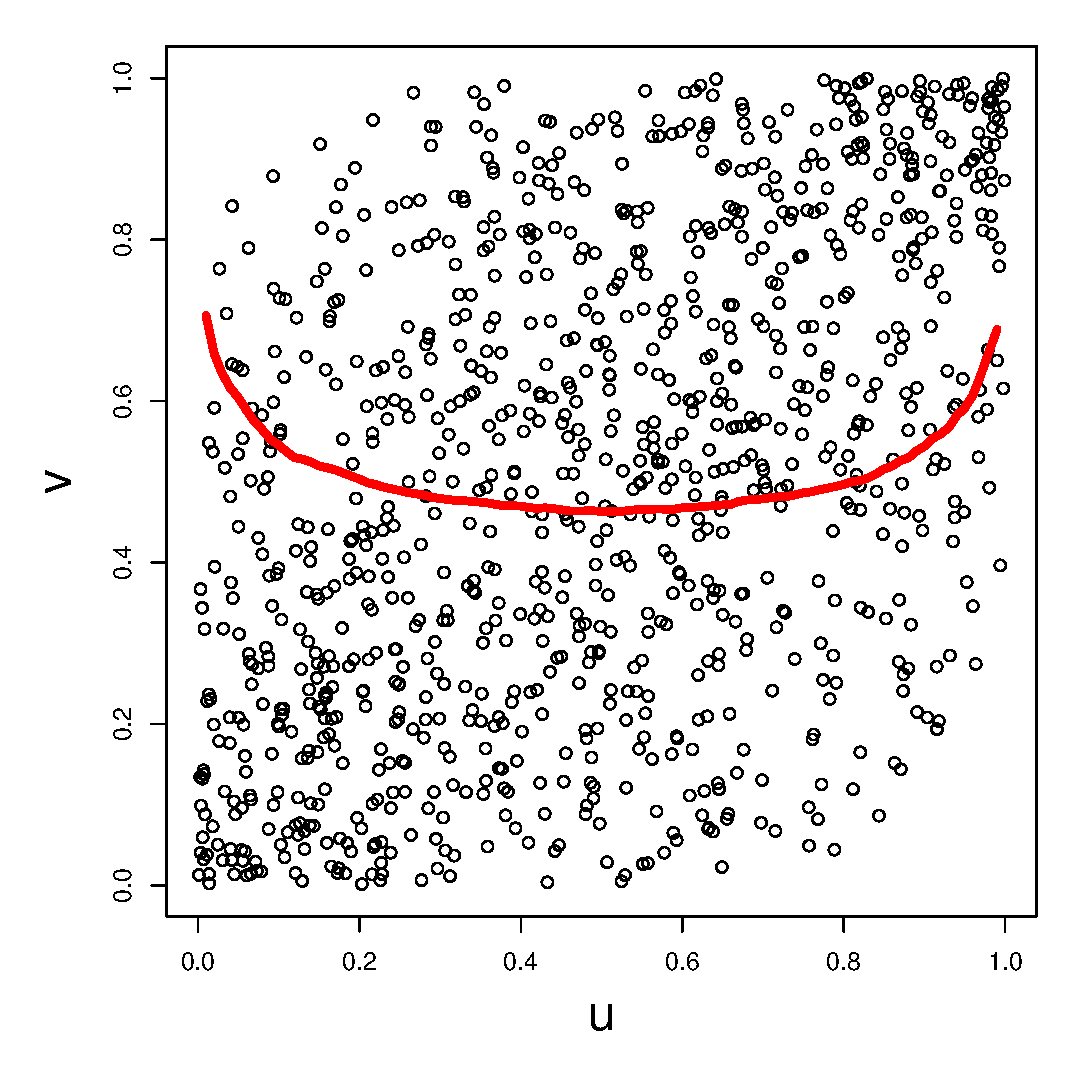
\includegraphics{factor1.eps}}
      \resizebox{60mm}{!}{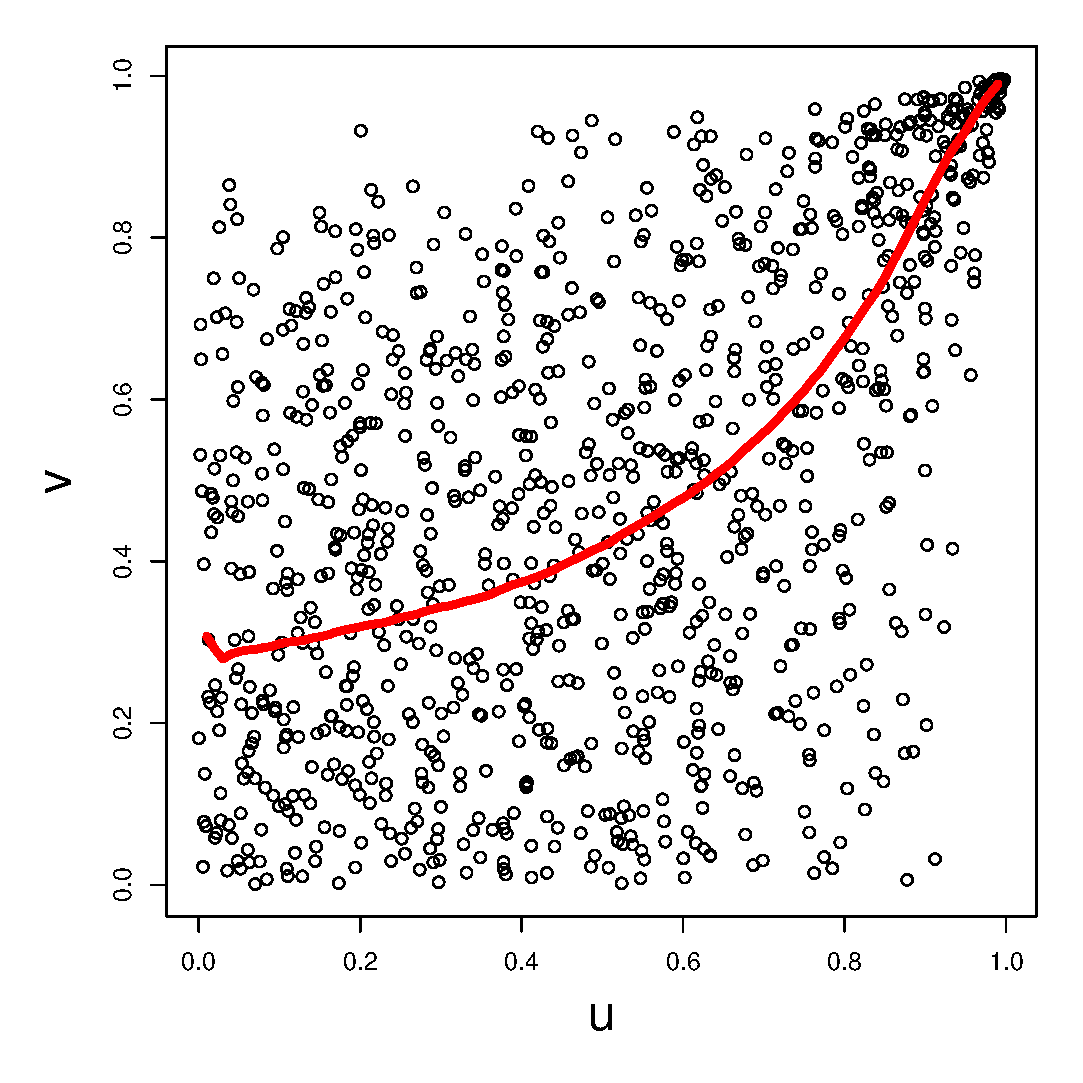
\includegraphics{factor2.eps}} \\
    \end{tabular}
    \caption{Simulated factor copulas and layer dependence curves assuming $s$ is standard normal (left panel) and $\chi^2_1$ (right panel).  }
    \label{ffactor}
  \end{center}
\end{figure}



The factor copula model generates positive layer dependence. Negative layer dependence is created by first simulating the corresponding positive layer dependence, and then taking complements of either percentile rank.

To generate a sample of $(u,v)$ of size $n$ from the factor copula model with layer dependence $\ell_\alpha$, $0\le\alpha\le 1$,  first simulate $\eps_i,\eta_i\sim N(0,1)$ for $i=1,\ldots,n$.  Arbitrarily initialise $s_i$ for $i=1,\ldots,n$ by setting it equal to a normal sample with standard deviation chosen such that $s_i+\eps_{i}$ and $s_i+\eta_{i}$ have Spearman's correlation consistent with $\ell_\alpha$. Then repeat:
\begin{enumerate}

\item Compute ``fitted"  $\hat\ell_{j/n}$ between  $(u_i,v_i)$ for $j=1,\ldots,n$, where $u_i$ and $v_i$ are calculated from the percentile ranks of $s_i+\eps_{i}$ and $s_i+\eta_{i}$, respectively.

\item Keep $s_1$ unchanged and update  $s_2,\ldots,s_n$ according to
$$
s_{i+1}  \leftarrow s_{i}+  \left(\frac{\ell_{i/n}}{\hat \ell_{i/n}}\right)^a(s_{i+1}-s_i)\cq a>0\;,
$$
in turn yielding an updated sample of $(u_i,v_i)$.

\item Go to 1 unless $\|\ell_{i/n} -  \hat\ell_{i/n} \|$ is less than some pre-specified small amount.

\end{enumerate}
Step 1 can be simplified by computing $\hat \ell_{j/n}$ over a fewer number of points and then fitting a parametric curve to computed values. The resulting sample $(u_i,v_i)$ for   $i=1,\ldots,n$ once the iteration is complete has  layer dependence $\hat\ell_\alpha\approx\ell_\alpha$.




\subsection{Illustration using stock returns}

The following illustrates layer dependence copula fitting using NASDAQ and FTSE returns. The top left panel in \fref{fmarketindex} plots percentile ranks of daily NASDAQ and FTSE returns from $1985$ and $2014$. Layer dependence  at every integer percentile and Spearman's correlation are shown in the same panel. Spearman's correlation is $0.4$, indicating moderate dependence between NASDAQ and FTSE returns. Layer dependence increases towards both tails, but more so in the lower tail. Hence major corrections in NASDAQ and FTSE tend to occur simultaneously, and negative corrections are more strongly dependent than positive corrections.

The top right panel in \fref{fmarketindex} fits a factor copula to a smooth layer dependence curve passing through empirical values\footnote{The smoothing is performed by fitting a polynomial of order 4 using least squares estimation.}. Simulated values of the fitted factor copula are shown in the same panel. The bottom left panel fits a Gaussian copula to past data by matching Spearman's correlation. The Gaussian copula has a symmetric layer dependence curve, and hence does not capture the stronger lower tail dependence exhibited in NASDAQ and FTSE data.  Student-$t$ and other elliptical copulas would suffer from the same inadequacy.

The bottom right panel in \fref{fmarketindex} plots the density of the common factor $s$ generating the fitted factor copula. Also shown is the density implicit in the fitted Gaussian copula. The density of $s$ is more peaked and left skewed, reflecting the stronger lower tail dependence and weak dependence in the centre.


\begin{figure}
  \begin{center}
    \begin{tabular}{cc}
      \resizebox{60mm}{!}{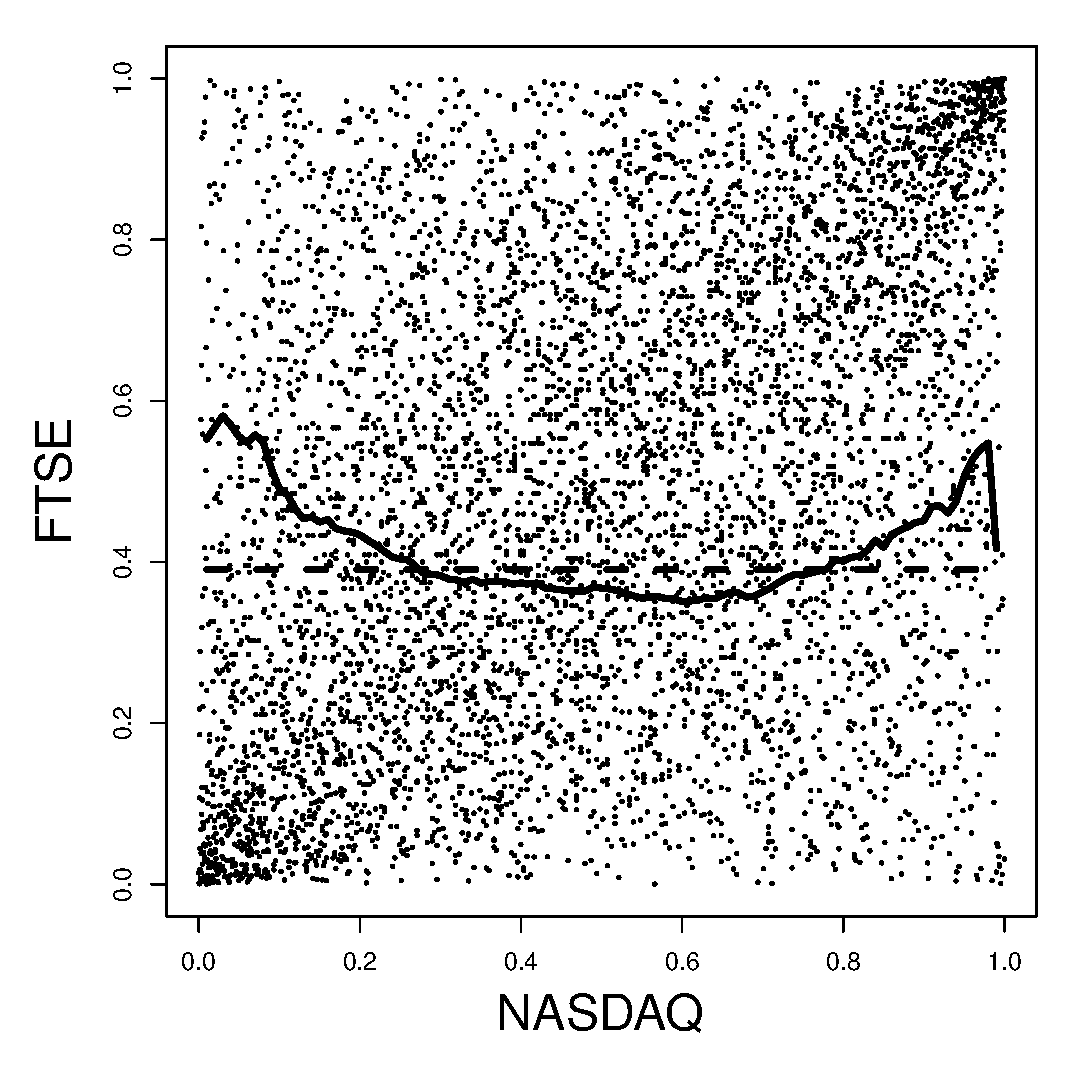
\includegraphics{NASDAQvsFTSE.eps}}
      \resizebox{60mm}{!}{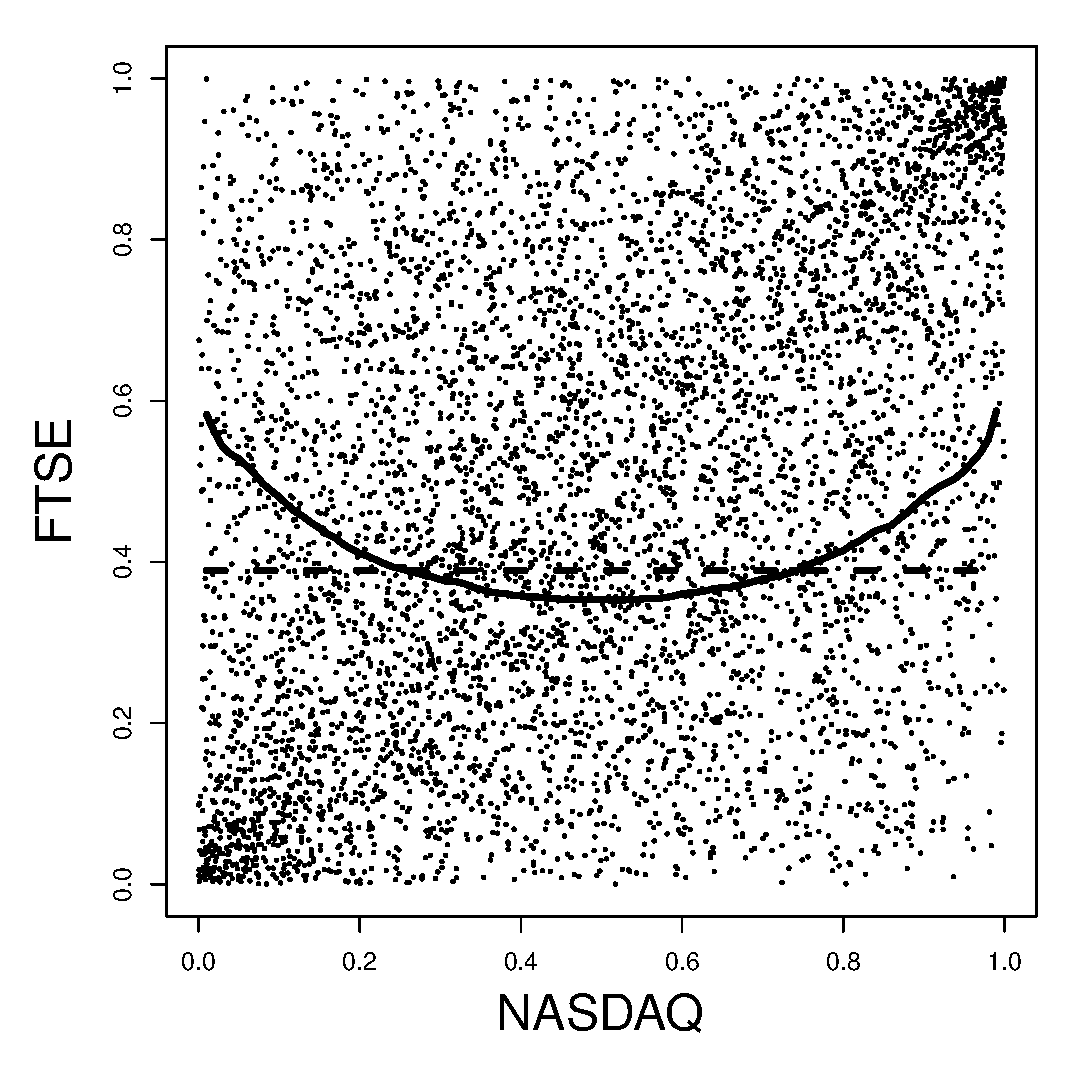
\includegraphics{NASDAQvsFTSE_fitted.eps}} \\
      \resizebox{60mm}{!}{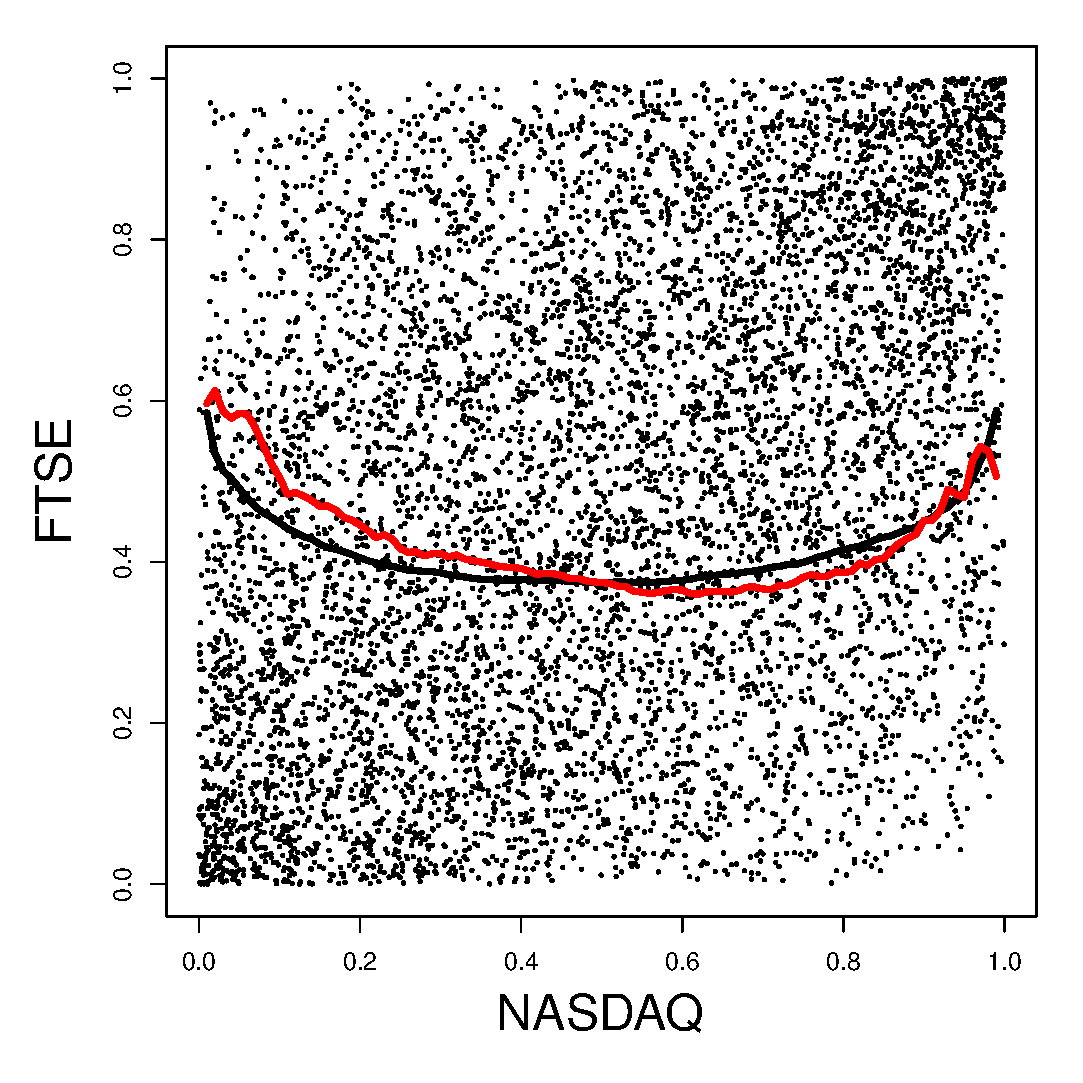
\includegraphics{gaussianfitted.eps}}
      \resizebox{60mm}{!}{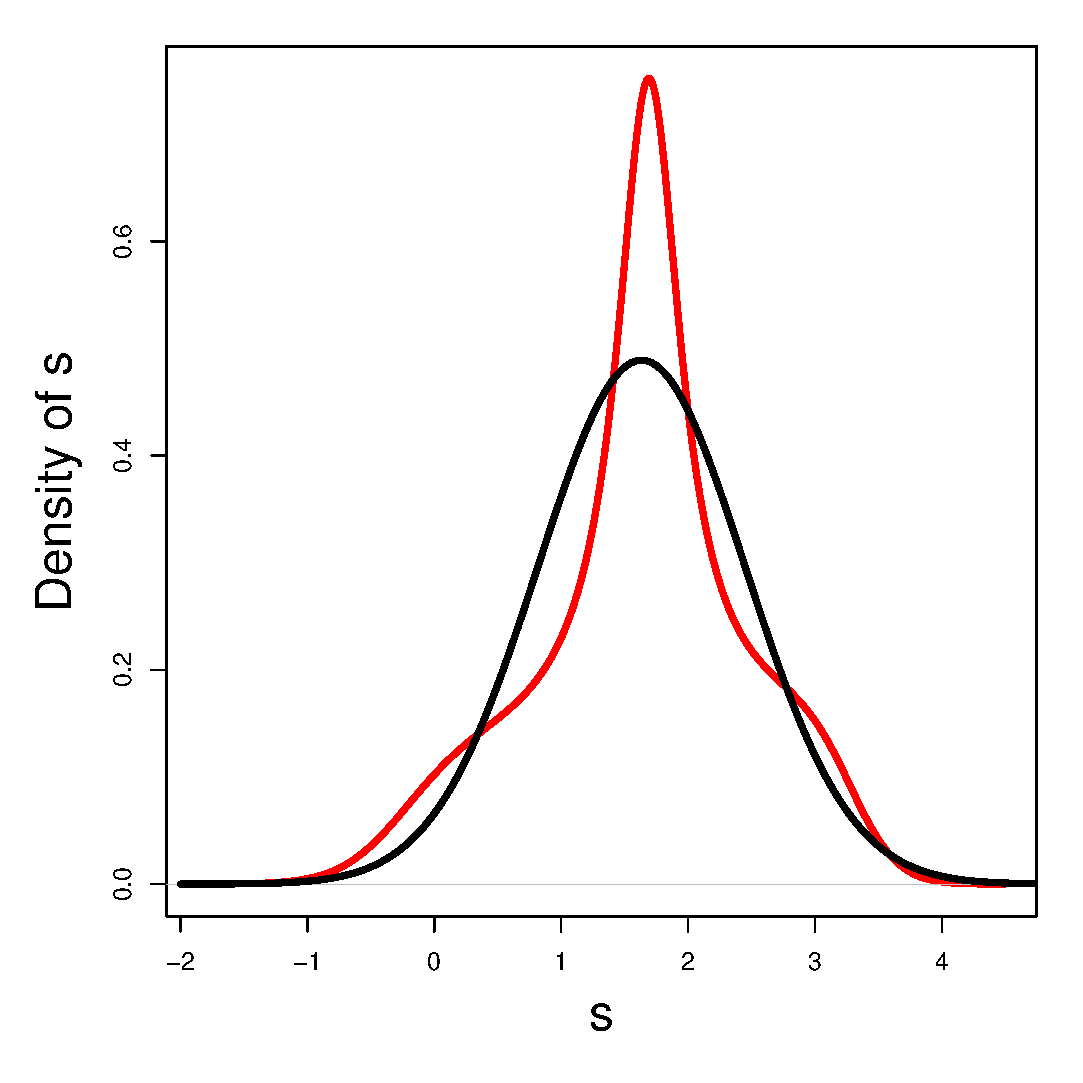
\includegraphics{densities.eps}} \\
    \end{tabular}
    \caption{The top left panel plots percentile ranks of NASDAQ and FTSE daily returns from 1985 to 2014, and the empirical layer dependence curve. The top right panel plots a parametrically smoothed layer dependence curve and a fitted factor copula. The bottom left panel plots a Gaussian copula and its layer dependence curve. The Gaussian copula is fitted by matching Spearman's correlation. The red empirical layer dependence curve is plotted in both panels containing fitted factor and Gaussian copulas. The bottom right panel graphs the density of $s$ underlying the fitted factor copula (red), and the implied density of $s$ underlying the Gaussian copula (black).}
    \label{fmarketindex}
  \end{center}
\end{figure}



\end{comment}


\begin{comment}
\subsection{Regression model}

The second approach exploits the relation $\tau_\alpha=(1+\alpha\ell_\alpha)/2$ where $\tau_\alpha$ is the upper conditional tail expectation $\E(v|u>\alpha)$.  Then
$$
\tau'_\alpha \equiv\frac{\de\E(v|u>\alpha)}{\de\alpha}= \frac{\de}{\de \alpha} \frac{\E\left\{v(u>\alpha)\right\}}{1-\alpha}
= \frac{\tau_\alpha-\mu_\alpha}{1-\alpha}\cq \mu_\alpha\equiv \E(v|u=\alpha)\;,
$$
where $\mu_\alpha$ is the regression curve of $v$ on $u$. Hence $\mu_\alpha=\tau_\alpha-(1-\alpha)\tau'_\alpha$
and $\tau_\alpha$ is monotonic if $\mu_\alpha$ is monotonic.

Suppose $\ell_\alpha$ and hence $\tau_\alpha$ is given for $\alpha=i/n$, $i=1,\ldots,n$ with values denoted $\tau_1,\tau_1,\ldots,\tau_{n}$.   Then  $C(u,v)$ with layer dependence $\ell_\alpha$ is simulated using
$$
v_i=F\{F^-(\mu_i)+\sigma\eps_i\}\ ,\ \mu_{i}=\tau_i - (n-i)(\tau_{i}-\tau_{i-1})\ ,\ \eps_i\sim N(0,1)\ ,\  i=1,\ldots,n\ ,
$$
with $\tau_0=1/2$ and $\sigma$ chosen so that Spearman's $\rho$ for the each sample is expected to match $\rho_S$ implied by $\ell_\alpha$ as in \eref{wtdaverage}.  Here $F$ is an appropriate distribution such as the normal or  logit:  $F^-(\mu_i)=\ln\{\mu_i/(1-\mu_i)\}$.  In the logic case setting $\sigma=1$ appears to ensure a match between the theoretical and empirical $\rho_S$.  To enforce the $v_1,\ldots,v_n$ are empirically uniform the final $F$ transformation $F$ is replaced by computing  empirical percentiles.
\end{comment}


\begin{comment}

\subsection{Measuring dependence asymmetry}

Dependence asymmetry is the difference between dependence in the upper tail compared to lower tail. Dependence asymmetry is important for example when modeling the sum of two random variables. Strong upper tail dependence relative to lower tail increases the right skewness of the sum since large outcome of both random variables are more likely to occur simultaneously.

Measure dependence asymmetry as $\ell^+-\ell^-$ where
$$
 \ell^+ \equiv \int_z^1 w_\alpha\ell_\alpha \de \alpha
\cq \ell^- = \int_0^{1-z} w_\alpha\ell_\alpha \de \alpha
\cq 0.5\leq z\leq 1\;,
$$
and $w_\alpha$ is a weighting function symmetric about $\alpha=0.5$. Hence dependence in the upper tail is the weighted average of layer dependence over percentiles above $z$, and dependence in the lower tail averages over percentiles below $1-z$ using identical weights. For example the Gaussian or $t$ copulas with symmetric dependence have $\ell^+-\ell^-=0$. For the Clayton copula, $\ell^+-\ell^-<0$ while $\ell^+-\ell^->0$ for the Gumbel copula.

Substituting the expression for $\ell_\alpha$ in \eref{definition} yields
$$
\ell^+
= \cov\left\{ v, \int_z^1 \frac{(u>\alpha)}{0.5\alpha(1-\alpha)} w_\alpha \de \alpha\right\}
=\cov\left\{v,(u>z)\int_z^u \frac{2w_\alpha}{\alpha(1-\alpha)} \de \alpha\right\}
$$
and similarly
$$
\ell^- =  \cov\left\{ v, \int_0^{1-z} \frac{(u>\alpha)}{0.5\alpha(1-\alpha)} w_\alpha \de \alpha\right\}
=\cov\left\{ v, (u\leq 1-z) \int_0^u \frac{2w_\alpha}{\alpha(1-\alpha)} \de \alpha \right\}
$$
$$
+\cov\left\{ v, (u> 1-z)  \right\} \int_0^{1-z}\frac{2w_\alpha}{\alpha(1-\alpha)} \de \alpha \;.
$$
\end{comment}

\begin{comment}

\section{Layer dependence between non--uniform random variables}\label{soriginal}


Consider random variables $x$ and $y$.  Analogous to \eref{definition}, define layer dependence between $x$ and $y$ as the scaled covariance between $y$ and $k$--layer of $x$:
$$
\ell_k^* \equiv \frac{\cov\{y,(x>k)\}}{\cov\{y^*,(x>k)\}} = \frac{\cor\{y,(x>k)\}}{\cor\{y^*,(x>k)\}}\;,
$$
where $k$ lies in the support of $x$, and $y^*$ has identical marginal distribution as $y$ and is comonotonic with $x$. The denominator hence ensures $\ell_k^*=1$ for all $k$ when $x$ and $y$ are comonotonic.

Layer dependence $\ell_k^*$ partially satisfies coherence properties of $\ell_\alpha$ in section \aref{scoherence}. If $x$ and $y$ are independent or comonotonic then $\ell_k^*=0$ and $1$, respectively, for all $k$. If $x$ and $y$ are countermonotonic then write $x=F^-(u)$ and $y=G^-(1-u)$ where $F^-$ and $G^-$ are inverse distribution functions of $x$ and $y$, respectively. Layer dependence in this case is
$$
\ell_k^*  =\frac{\cov\{G^-(1-u),(u>\alpha)\}}{\cov\{G^-(u),(u>\alpha)\}} \leq 0 \cq \alpha=F(k) \;,
$$
reducing to $-1$ if $G^-$ is symmetric: $G^-(1-u)-G(0.5)=G(0.5)-G(u)$. Layer dependence $\ell_k^*$ also preserves correlation order: if $x$ and $y$ increase in correlation order in the sense of \cite{dhaene2009correlation} then $\ell_k^*$ is higher for all $k$, since higher correlation order translates to higher covariance values. Layer dependence $\ell_k^*$ is symmetric if the distribution of $y$ is symmetric.

Averaging $\ell_k^*$ yields a link to correlation between $x$ and $y$:
$$
\int \frac{\cov\{y^*,(x>k)\}}{\cov(y^*,x)} \ell^*_k \de k =  \frac{\int \cov\{y,(x>k)\} \de k}{\cov(y^*,x)}
= \frac{\cov(x,y)}{\cov(x,y^*)} = \frac{\cor(x,y)}{\cor(x,y^*)}
$$
applying the result in \eref{decompose}.

The four panels \fref{foriginalscale} calculate layer dependence curves between $x$ and $y$ with combinations of symmetric and right skewed beta marginal distributions. A Gumbel copula is assumed. Layer dependence between percentile ranks is included for comparison. Layer dependence retains its overall shape when observed random variables are used instead of percentile ranks.

\begin{figure}
  \begin{center}
    \begin{tabular}{cc}
      \resizebox{60mm}{!}{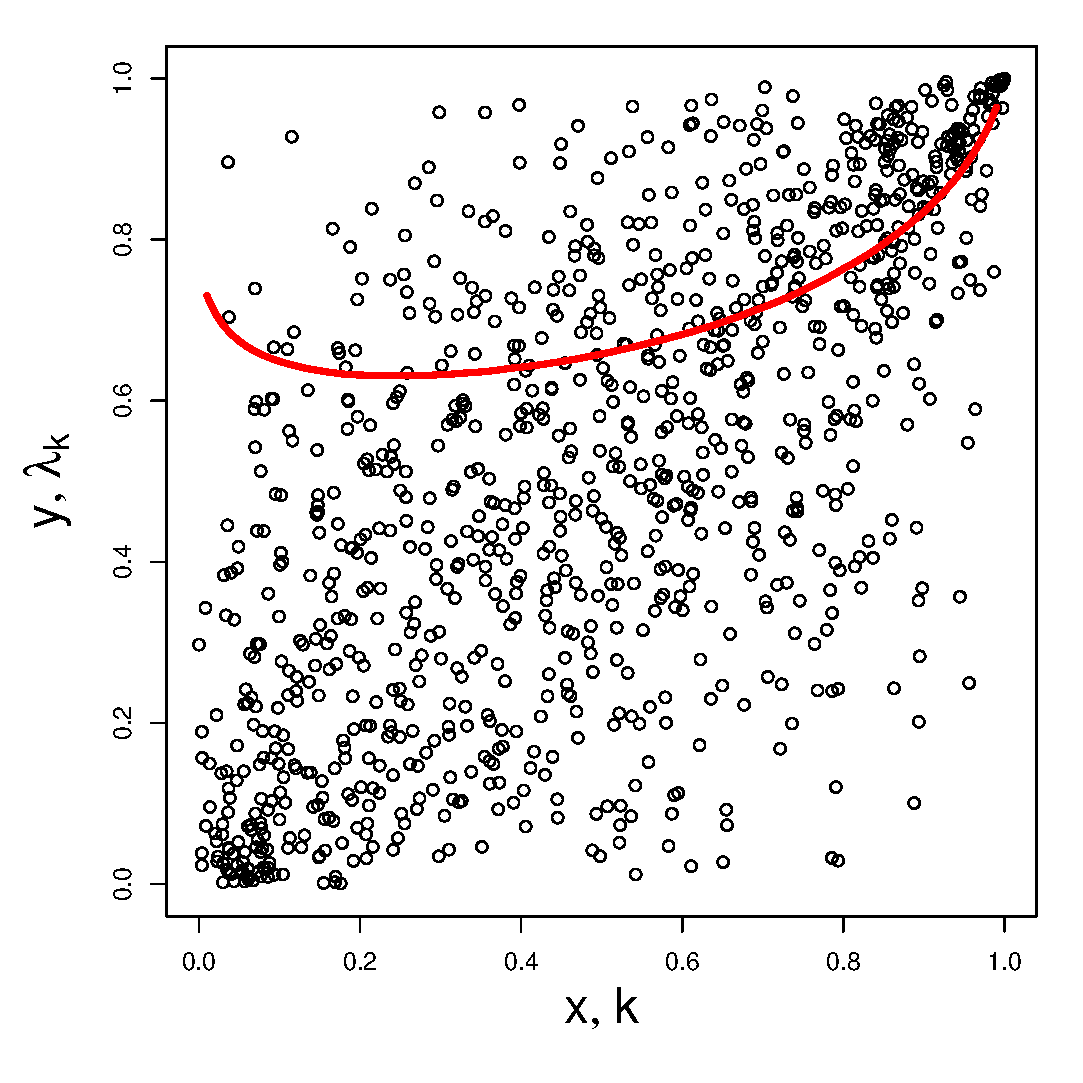
\includegraphics{gumbel0.eps}}
      \resizebox{60mm}{!}{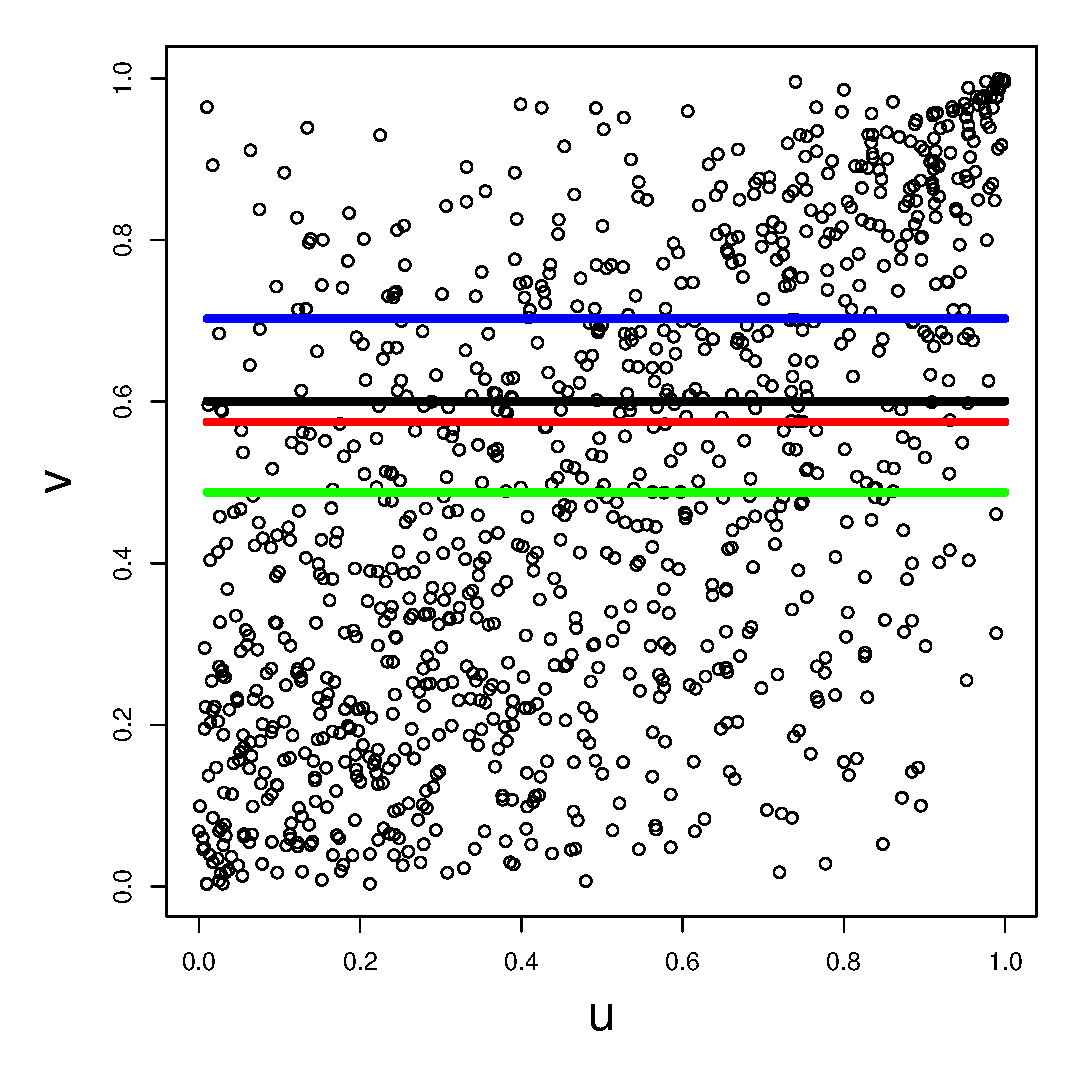
\includegraphics{gumbel1.eps}} \\
      \resizebox{60mm}{!}{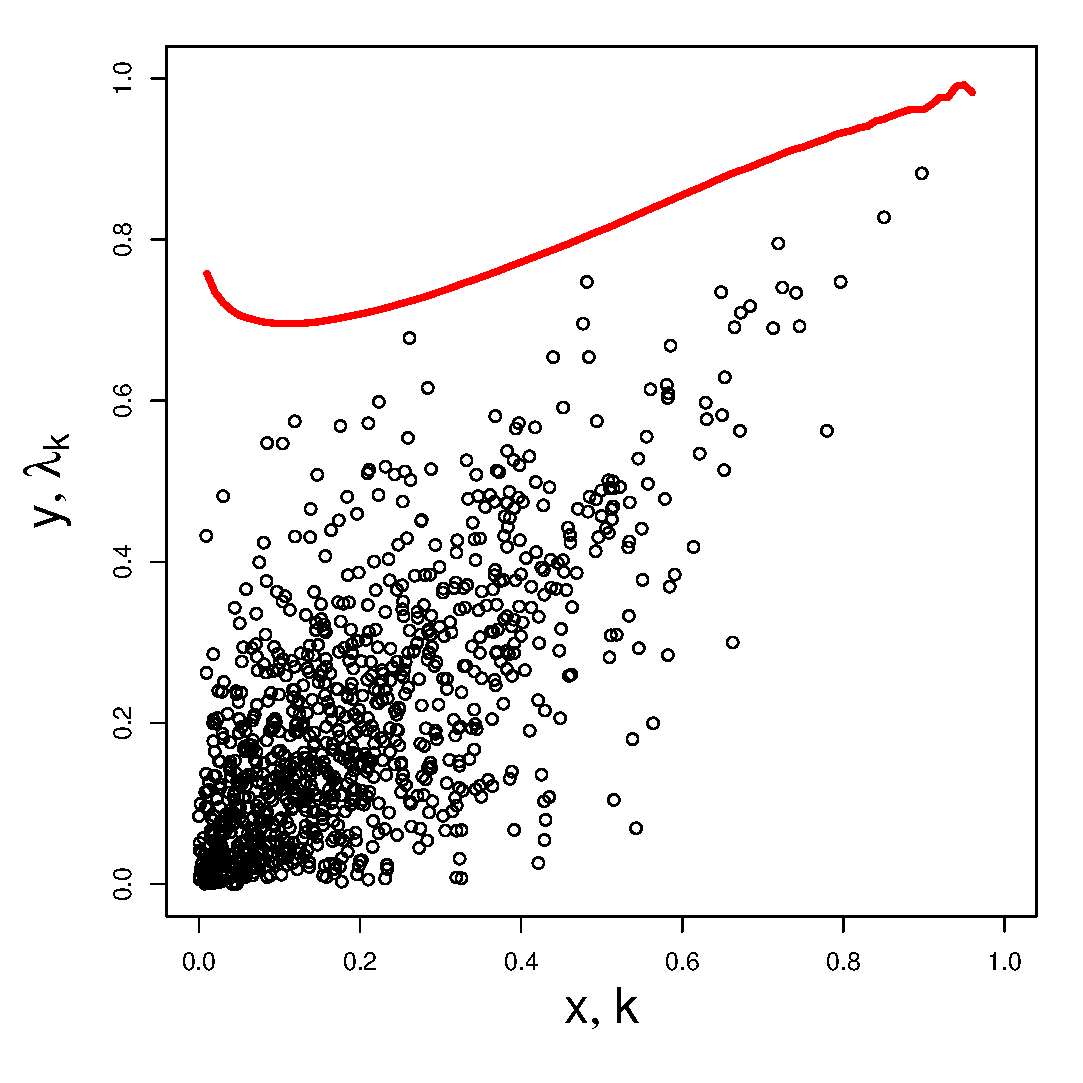
\includegraphics{gumbel2.eps}}
      \resizebox{60mm}{!}{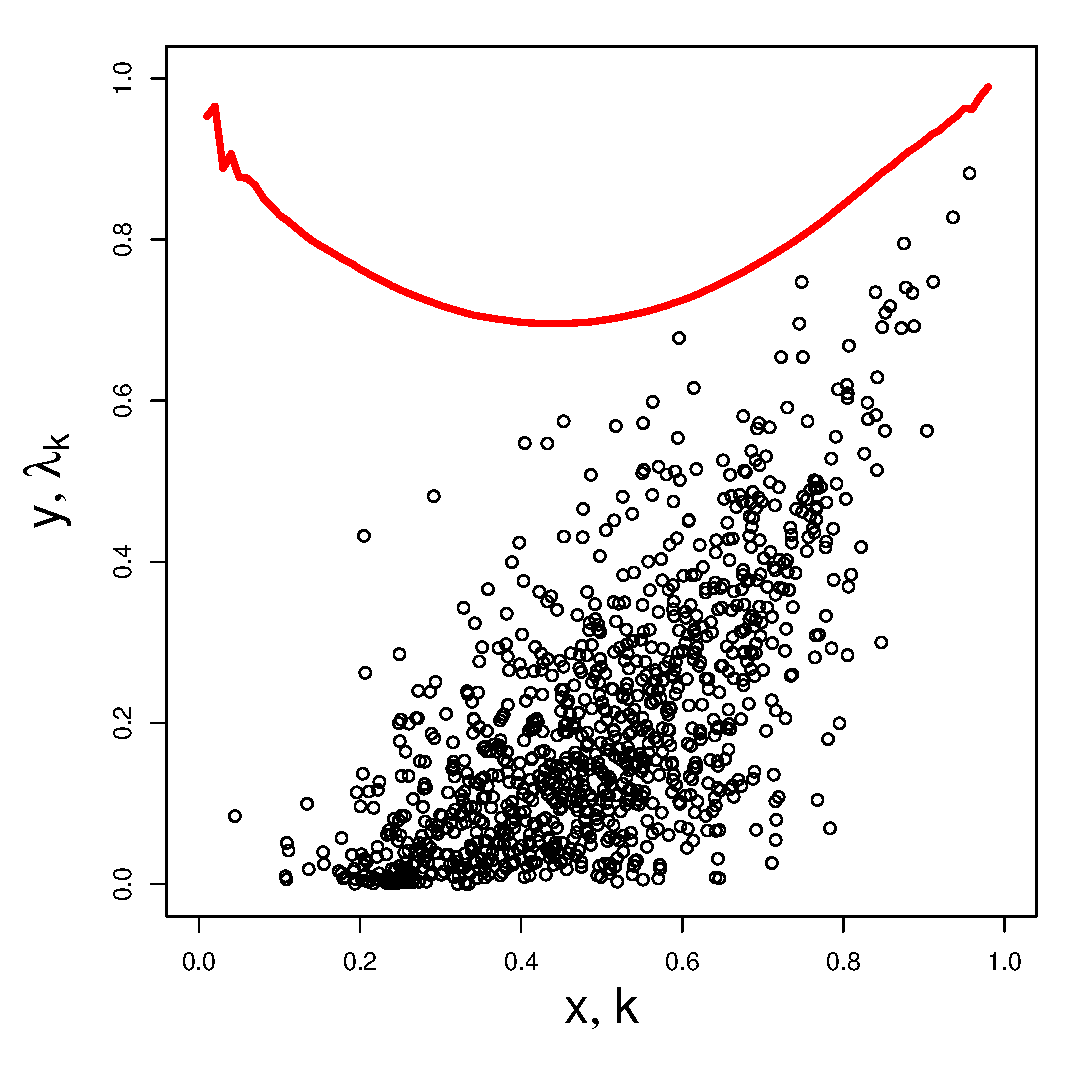
\includegraphics{gumbel3.eps}} \\
    \end{tabular}
    \caption{Layer dependence curves between $x$ and $y$ (red line) for a Gumbel copula. The top left panel assumes uniform $x$ and $y$, yielding original layer dependence. The top right panel assumes symmetric $x$ and $y$. The bottom left panel assumes right skewed $x$ and $y$. The bottom right panel assumes symmetric $x$ and right skewed $y$.}
    \label{foriginalscale}
  \end{center}
\end{figure}

\end{comment}


\begin{comment}
\subsection{Gap between conditional tail expectations}

Manipulating layer dependence $\ell_\alpha^*$ yields
$$
\ell_\alpha^* = \frac{\E(y|x>V_\alpha)-\E(y|x\leq V_\alpha)}{\E(y^*|x>V_\alpha)-\E(y^*|x\leq V_\alpha)}
=\frac{\E(y|u>\alpha)-\E(y|u\leq\alpha)}{\E(y^*|u>\alpha)-\E(y^*|u\leq\alpha)} \;,
$$
the gap between upper and lower conditional tail expectations of $y$. A similar expression for original layer dependence $\ell_\alpha$ exists in \eref{gapexp}, where conditional tail expectations of percentile rank $v$ are evaluated instead of $y$.

Using the income-education example in \sref{sintroduction}, the population is again divided into two segments depending on whether education is below or above the $\alpha$-percentile. Average actual income is measured in each segment rather than average income ranking. The calculated gap in average actual income is divided by the maximum gap, or the difference between average actual income above and below the $\alpha$-percentile.


\subsection{Link to Pearson correlation}

Taking the following weighted average of $\ell_\alpha^*$ yields scaled Pearson correlation between $x$ and $y$:
$$
\int_0^1 \ell_\alpha^* \left[\frac{\cov\{y^*,(u>\alpha)\}V_\alpha'}{\cov(y^*,x)} \right] \de \alpha
= \frac{\cov\left\{y, \int_0^1 (u>\alpha)V_\alpha' \de \alpha \right\}}{\cov(y^*,x)} =\frac{\cov(y,V_u)}{\cov(y^*,x)}
$$
$$
= \frac{\cor(y,x)}{\cor(y^*,x)}
\cq \int_0^1 \frac{\cov\{y^*,(u>\alpha)\}V_\alpha'}{\cov(y^*,x)}  \de \alpha= \frac{\cov(y^*,V_u)}{\cov(y^*,x)} = 1 \;,
$$
where weights integrate to one. The denominator $\cor(y^*,x)$ in scaled Pearson correlation ensures unity if $x$ and $y$ are comonotonic. Similarly a weighted average of layer dependence $\ell_\alpha$ over all $\alpha$, using quadratic weights, yields  $\rho_S$ as shown in \eref{wtdaverage}.

\subsection{Relationship between two layer dependences}

layer dependences between original random variables and between their percentile ranks are generated by a common ``dependence generating function"
$$
g_{\alpha,\beta}\equiv \frac{\cov\{(u>\alpha,v>\beta)\}}{\cov\{(u>\alpha,u>\beta)\}}
= \frac{C(\alpha,\beta)-\alpha\beta}{\min(\alpha,\beta)-\alpha\beta}  \cq 0\leq \alpha,\beta\leq 1\;,
$$
where $C$ is the copula underlying $(u,v)$. The dependence generating function $g_{\alpha,\beta}$ measures dependence between $\alpha$-layer of $x$ and $\beta$-layer of $v$. In particular $g_{\alpha,\beta}=1$ for all $\alpha$ and $\beta$ if $u$ and $v$ are perfectly dependent, and $g_{\alpha,\beta}=0$ if $u$ and $v$ are independent. Negative dependence yields negative $g_{\alpha,\beta}$.

Taking a weighted average of $g_{\alpha,\beta}$ over all $\beta$ yields layer dependence, between percentile ranks and between observed random variables. Layer dependence $\ell_\alpha$ is generated by the weighted integral
$$
\ell_\alpha= \int_0^1 w_{\beta,1} g_{\alpha,\beta} \de\beta
\cq w_{\beta,1}=\frac{\min(\alpha,\beta)-\alpha\beta}{\int_0^1 \{\min(\alpha,\beta)-\alpha\beta\}\de\beta}
=\frac{\min(\alpha,\beta)-\alpha\beta}{0.5\alpha(1-\alpha)}
$$
and layer dependence $\ell_\alpha^*$ is generated by a different weighted integral
$$
\ell_\alpha^* = \int_0^1 w_{\beta,2}   g_{\alpha,\beta} \de G^-(\beta)
\cq w_{\beta,2}=\frac{\min(\alpha,\beta)-\alpha\beta}{\int_0^1 \{ \min(\alpha,\beta)-\alpha\beta\}\de G^-(\beta)}
$$
$$
=\frac{\min(\alpha,\beta)-\alpha\beta}{\cov \{G^-(u),(u>\alpha)\}}  \;.
$$
For $\ell_\alpha^*$, weights attached to $g_{\alpha,\beta}$ are proportional to the derivative $(G^-)'$. Hence $g_{\alpha,\beta}$ is weighted more heavily over values of $\beta$ where the derivative $\{G^-(\beta)\}'$ is large, such as in the tail of a right skewed distribution. In comparison weights for layer dependence $\ell_\alpha$ are ``marginal free."

The dependence generating function captures complete dependence information due to its direct relationship with the copula $C$. Correlations $\cor(u,v)$ and $\cor(x,y)$ show completely summarised dependence information. Layer dependences $\ell_\alpha$ and $\ell_\alpha^*$ balances the extremes and shows dependence information on a single dimension.

\end{comment}



\begin{comment}

\section{Comparison with existing local dependence measures}\label{sliterature}

This section compares layer dependence with existing local dependence measures: tail concentration \citep{venter2002tails}, correlation curve \citep{bjerve1993correlation}, and bivariate measures by \cite{bairamov2003new}, \cite{jones1996local} and \cite{holland1987dependence}. Calculations are applied to copulas in \fref{fillustration}. Layer dependence is more reflective of local dependence (dispersion and concordance between points), and satisfies all five coherence properties in \sref{scoherence}. In addition there is a direct relationship between layer dependence and  $\rho_S$ in \eref{wtdaverage}.



\subsection{Tail concentration}

\cite{venter2002tails} defines tail concentration at $0\leq\alpha\leq 1$ by combining lower and upper conditional tail probabilities relative to $\alpha$:
\begin{equation}\label{tailcon}
\tau_\alpha \equiv (\alpha\leq 0.5) \p(v\leq \alpha|u\leq \alpha) + (\alpha>0.5)\p(v>\alpha|u>\alpha) \;.
\end{equation}
Higher tail concentration implies $u$ and $v$ are more likely to fall in the same lower tail ($\alpha\leq 0.5$) or upper tail ($\alpha>0.5$). Tail concentration partially satisfies coherence properties described in \sref{scoherence}, and partially reflects local dependence. Layer dependence refines tail concentration through standardisation and reflecting average dispersion between discordant points. Further discussion of tail concentration is shown below.

Rewrite tail concentration in terms of the copula $C$ of $(u,v)$:
$$
\tau_\alpha = (\alpha\leq 0.5)\frac{C(\alpha,\alpha)}{\alpha}+(\alpha>0.5)\frac{1-2\alpha+C(\alpha,\alpha)}{1-\alpha} \;,
$$
therefore tail concentration depends only on the diagonal section of the copula, and is hence symmetric in $u$ and $v$. Independence implies $\tau_\alpha=\alpha(\alpha\leq 0.5)+(1-\alpha)(\alpha>0.5)$, and comonotonicity and countermonotonicity yield $\tau_\alpha=1$ and $\tau_\alpha=0$, respectively. Hence tail concentration does not satisfy independence and perfect dependence (countermonotonicity) coherence properties. Symmetry is also not satisfied since tail concentration is non-negative. The ordering property is satisfied since tail concentration increases with the copula $C$. Lastly $0\leq\tau_\alpha\leq 1$ since $\tau_\alpha$ is a probability, hence the bounds property holds.

Standardising tail concentration improves its coherence and reflection of local dependence. The latter is demonstrated via an illustration below. Standardisation involves subtracting the value assuming independence, and dividing the result by its maximum value:
$$
\tau_\alpha^* \equiv \frac{\tau_\alpha - \{\alpha(\alpha\leq 0.5)+(1-\alpha)(\alpha>0.5)\}}{1-\{\alpha(\alpha\leq 0.5)+(1-\alpha)(\alpha>0.5)\}}
=\frac{C(\alpha,\alpha)-\alpha^2}{\alpha(1-\alpha)} = \gamma_\alpha \;.
$$
Standardised tail concentration $\tau_\alpha^*=0$ if $u$ and $v$ (independence property), and is negative if $u$ and $v$ are negatively dependent. Standardised tail concentration is also equal to the measure of concordance $\gamma_\alpha$ defined in \eref{concordance}.

From \eref{decomposition}, layer dependence combines standardised tail concentration $\tau_\alpha^*=\gamma_\alpha$ and average dispersion between discordant points $\delta_\alpha$. Hence layer dependence refines tail concentration in two ways:
\begin{itemize}

\item layer dependence includes standardisation to achieve coherence. Standardisation also yields a more accurate reflection of local dependence.

\item layer dependence reflects average dispersion between discordant $u$ and $v$, yielding additional accuracy in local dependence measurement.
\end{itemize}
\fref{fventerillustration} demonstrates the above refinements by comparing tail concentration, its standardised value and layer dependence using identical copulas as \fref{fillustration}. Tail concentration, without standardisation, does not always trace local dependence. For example tail concentration decreases at the upper tail of the Gumbel copula, despite upper tail dependence. Similarly for the Clayton copula. Standardisation corrects these inconsistencies. Layer dependence further refines the calculation by reflecting dispersion between discordant points. For example layer dependence increases to one at the upper tail of the Gumbel copula and lower tail of the Clayton copula, whereas standardised tail concentration does not increase completely to one, despite the presence of tail dependence. In addition standardised tail concentration decreases significantly at both tails of Guassian and Frank copulas although there is no increased dispersion of $(u,v)$ in those areas.
\begin{figure}
  \begin{center}
    \begin{tabular}{cc}
      \resizebox{60mm}{!}{\includegraphics{vnormal.eps}}
      \resizebox{60mm}{!}{\includegraphics{vgumbel.eps}} \\
      \resizebox{60mm}{!}{\includegraphics{vclayton.eps}}
      \resizebox{60mm}{!}{\includegraphics{vfrank.eps}} \\
    \end{tabular}
    \caption{Calculation of tail concentration (blue line) for a Gaussian copula (top left), Gumbel copula (top right), Clayton copula (bottom left) and Frank copula (bottom right). Standardised values (dotted line) and layer dependence (red line) are also shown in each panel.}
    \label{fventerillustration}
  \end{center}
\end{figure}



\subsection{Correlation curve}

\cite{bjerve1993correlation} defines correlation curve based on the conditional distribution of $v$ given $u$. Correlation curve has similar values and coherence properties as layer dependence. However calculated values of correlation curve are volatile due to reliance on a ``pointwise" conditional distribution.

From \cite{bjerve1993correlation}, the correlation curve of $v$ with respect to $u$ at $\alpha$ is defined as
$$
c_\alpha \equiv \frac{\sigma\mu_\alpha'}{\sqrt{(\sigma\mu_\alpha')^2+\sigma_\alpha^2}} = \sign(\mu_\alpha') \times \frac{1}{\sqrt{1+s_\alpha^2}}
\cq 0\leq\alpha\leq 1 \;,
$$
$$
s_\alpha^2\equiv \left(\frac{\sigma_\alpha}{\mu_\alpha'\sigma}\right)^2  \cq \sigma^2\equiv \var(v) \cq \sigma_\alpha^2\equiv \var(v|u=\alpha)
\cq \mu_\alpha\equiv \E(v|u=\alpha) \;.
$$
where $\mu_\alpha$ and $\sigma_\alpha^2$ are the conditional mean and variance of $v$ at $u=\alpha$, respectively, and $\sigma^2=1/12$ is the unconditional variance of $v$. In addition $\mu_\alpha'$ is the derivative of $\mu_\alpha$ with respect $\alpha$. \cite{bjerve1993correlation} also generalises the correlation curve by replacing mean and variance with other location and scale measures such as median and interquartile range, respectively.


The correlation curve $c_\alpha$ at any $\alpha$ is affected by two factors: the derivative $\mu'_\alpha$ and the ratio $\sigma_\alpha^2/\sigma^2$. The former is the sensitivity of the conditional mean of $v$ to changes in $u=\alpha$. Higher sensitivity implies stronger local dependence between $u$ and $v$, increasing $c_\alpha$. The second is the conditional variance of $v$ relative to the unconditional variance. A higher ratio implies values of $v$ conditional on $u=\alpha$ are more variable, hence the conditional mean of $v$ at $u=\alpha$ is a less satisfactory predictor of $v$. The result is lower local dependence and $c_\alpha$.


Correlation curve satisfies similar coherence properties as layer dependence. In particular, for all $\alpha$, $-1\leq c_\alpha\leq 1$ and $c_\alpha=-1$, $0$ and $1$ if $u$ and $v$ are countermonotonic, independent and comonotonic, respectively. Replacing $u$ or $v$ with its complement reverse the sign of $c_\alpha$. In addition $c_\alpha$ increases when $u$ and $v$ are more ``regression dependent.'' \cite{bjerve1993correlation} further discusses properties of correlation curves.


\fref{fcorcurve} graphs correlation curves using identical copulas as \fref{fillustration}. Layer dependence is included as a comparison. Correlation curve varies similarly as layer dependence in all four copulas. However values of correlation curve are volatile, despite a large sample size of $10$ million. In comparison calculations of layer dependence in \fref{fillustration} utilises a $100000$-sample. The volatile correlation curve is due to involvement of conditional means, the derivative, and conditional variances at specific values of $u$.
\begin{figure}
  \begin{center}
    \begin{tabular}{cc}
      \resizebox{60mm}{!}{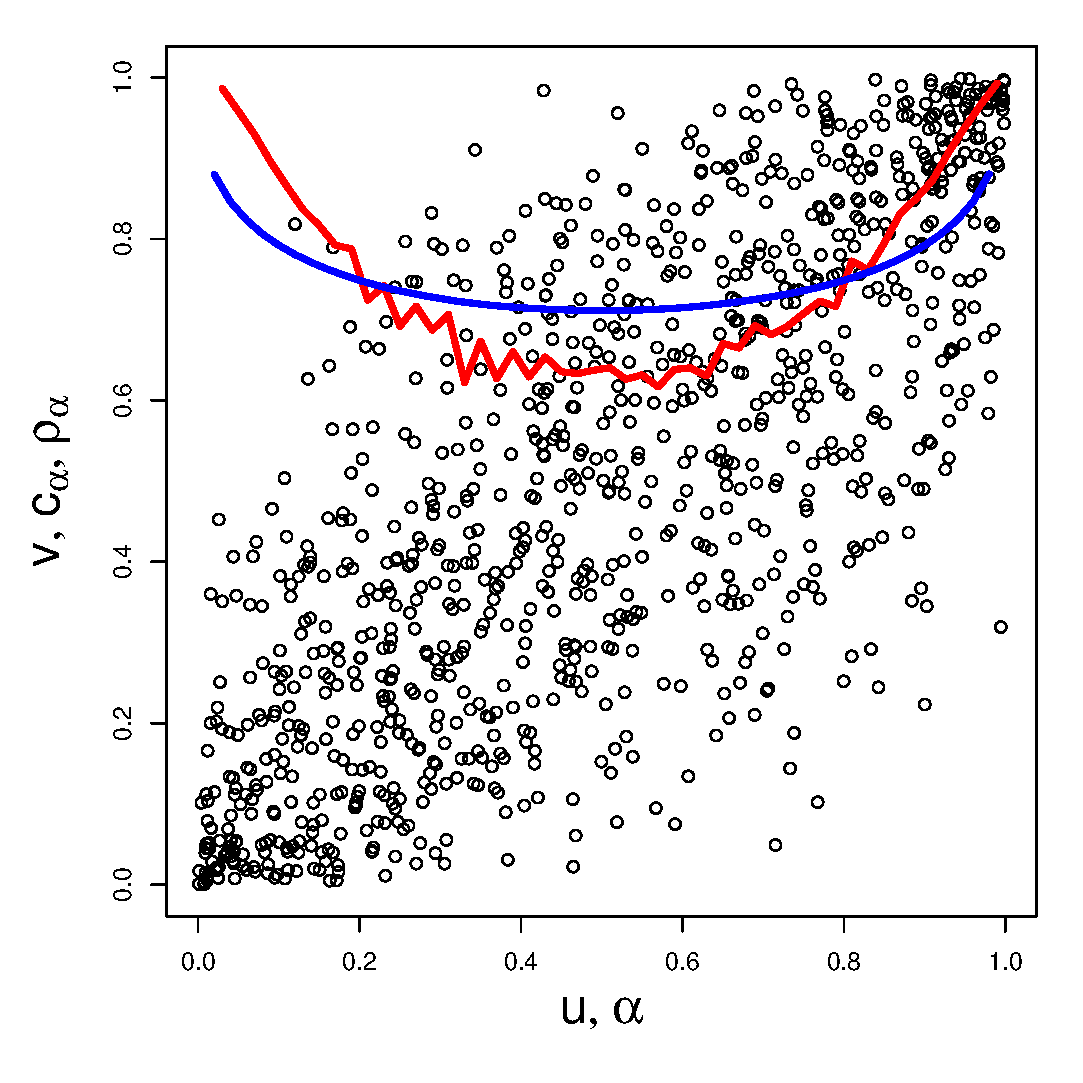
\includegraphics{cnormal.eps}}
      \resizebox{60mm}{!}{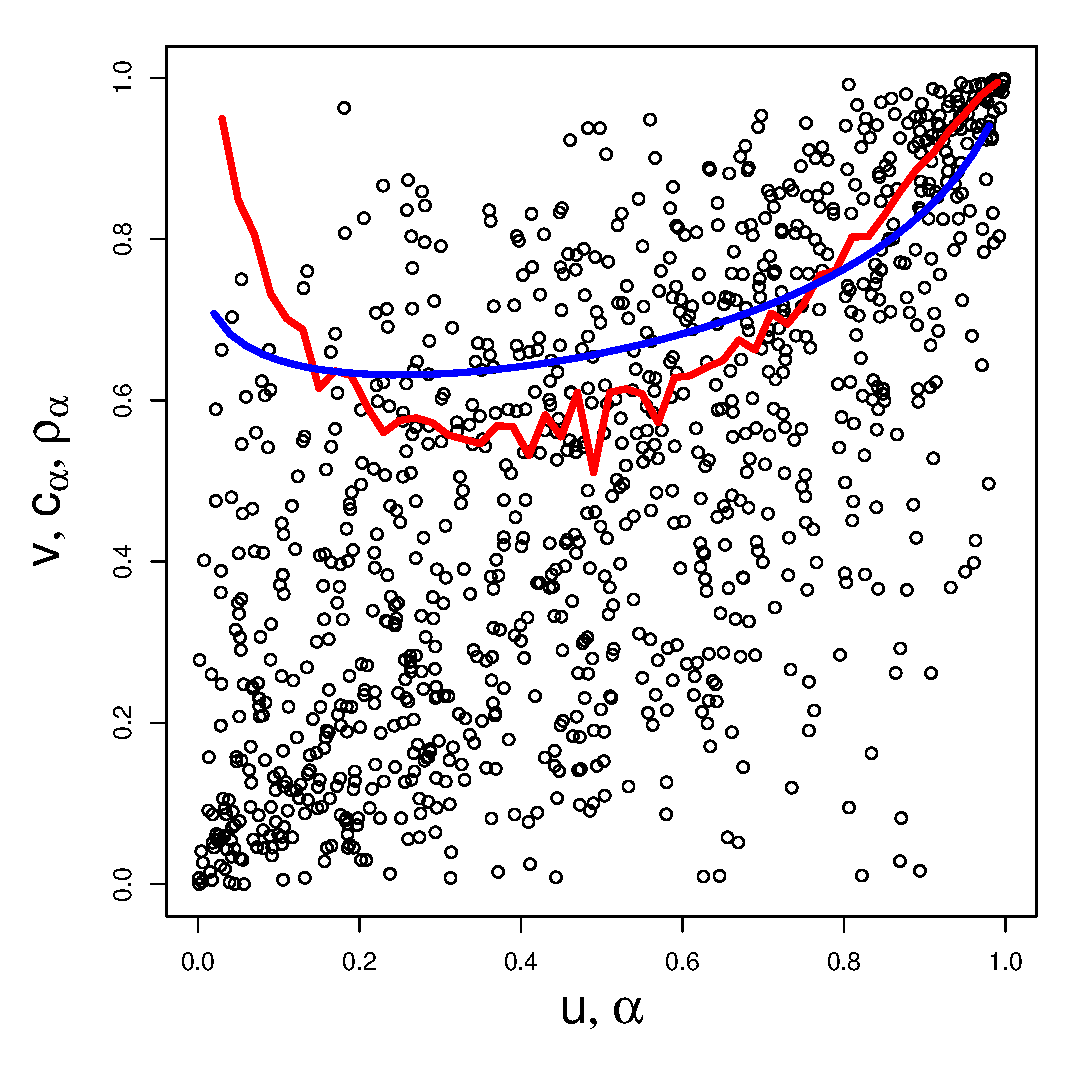
\includegraphics{cgumbel.eps}} \\
      \resizebox{60mm}{!}{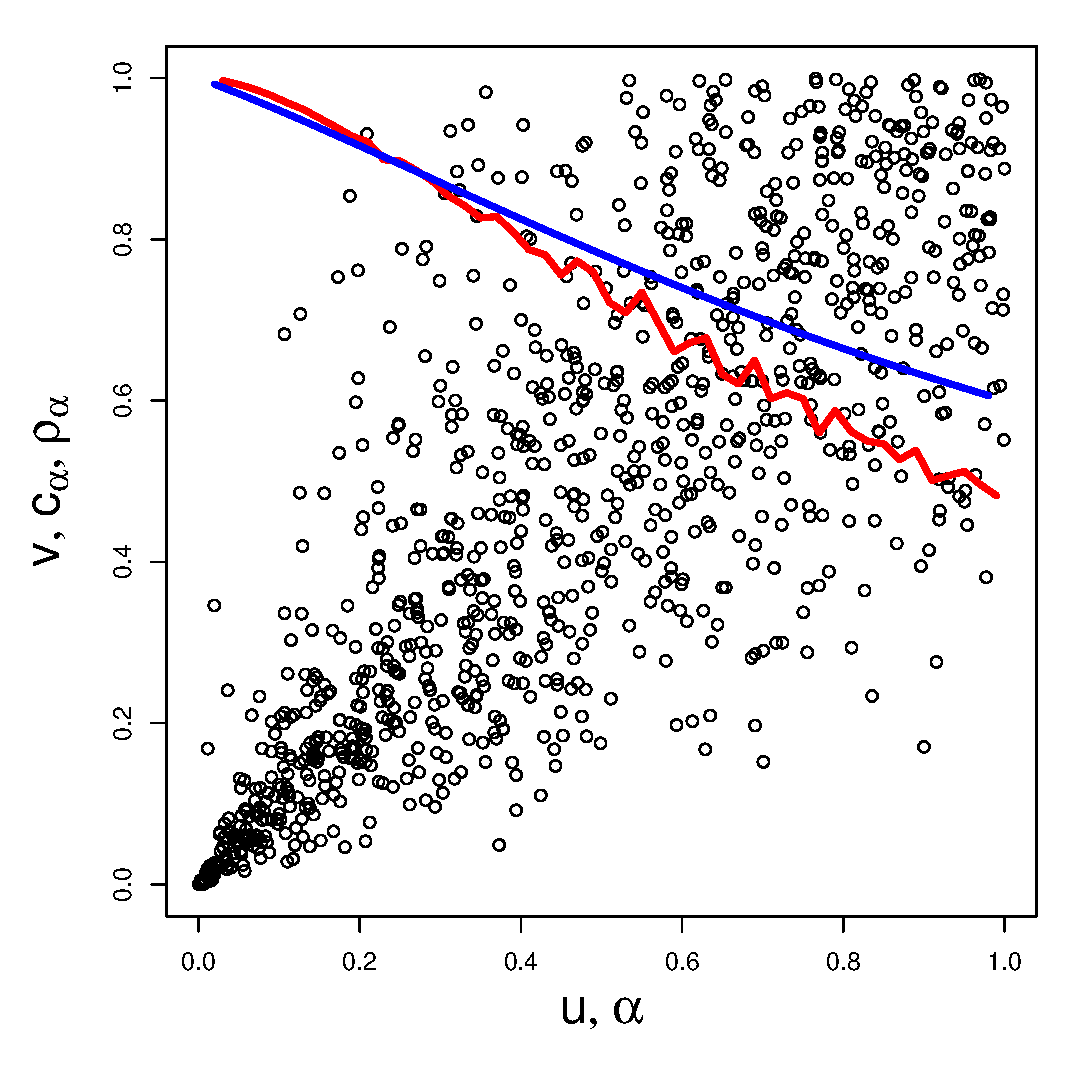
\includegraphics{cclayton.eps}}
      \resizebox{60mm}{!}{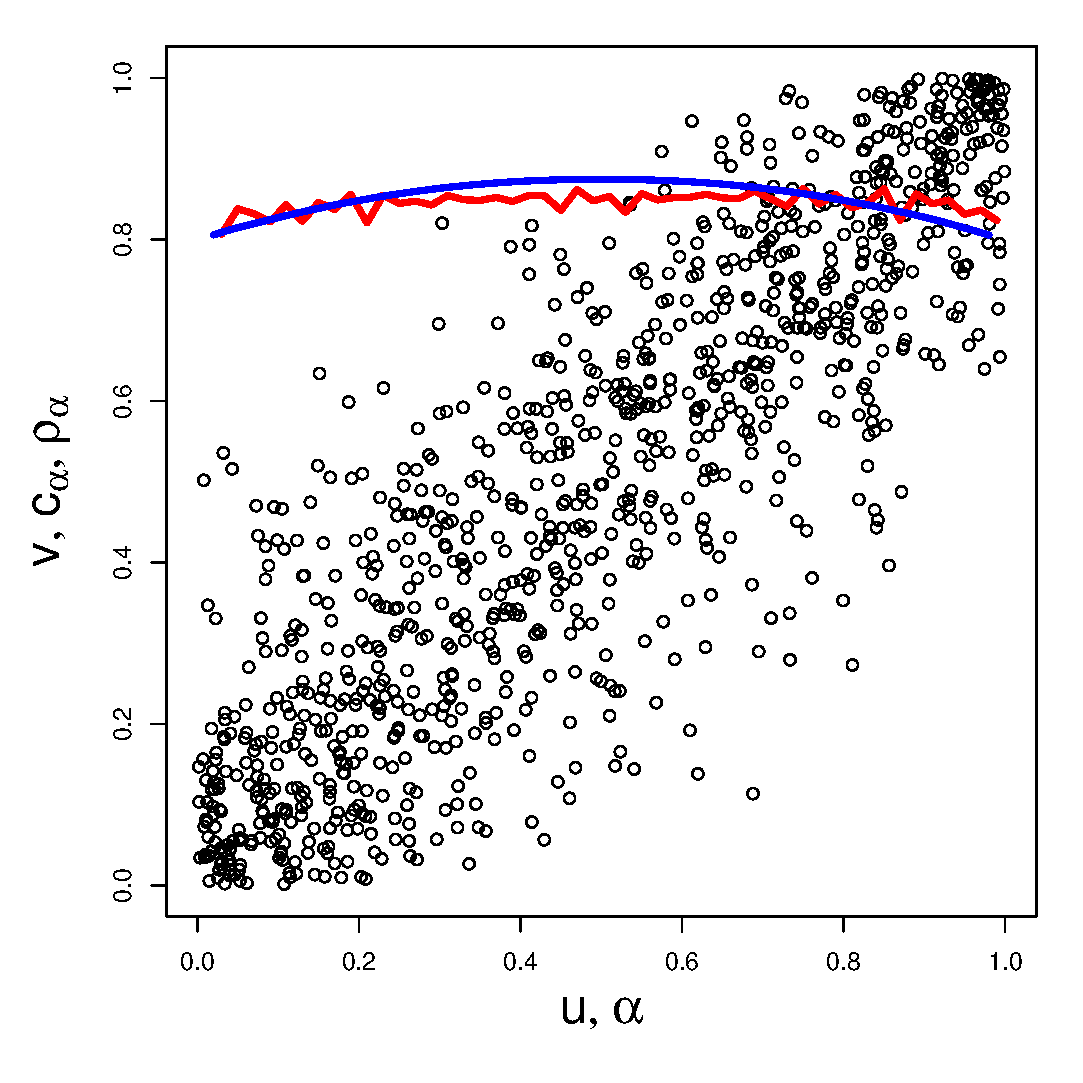
\includegraphics{cfrank.eps}} \\
    \end{tabular}
    \caption{Calculation of correlation curve (red line) for a Gaussian copula (top left), Gumbel copula (top right), Clayton copula (bottom left) and Frank copula (bottom right). Layer dependence (blue line) is also shown in each panel.}
    \label{fcorcurve}
  \end{center}
\end{figure}


\subsection{Bivariate local dependence measures}

\cite{bairamov2003new} defines a bivariate local dependence function, measuring dependence at various values of $(u,v)$, by generalising  $\rho+S$ using first and second order conditional expectations. \cite{jones1996local} and \cite{holland1987dependence} also define a bivariate local dependence function, based on partial derivatives of the log joint density function. Bivariate local dependence functions maintain the dimension of a bivariate joint distribution, and are less graphically interpretable than univariate local dependence functions such as layer dependence, tail concentration and correlation curve. In addition whilst the local dependence by \cite{bairamov2003new} is constrained in $[-1,1]$, the local dependence function by \cite{jones1996local} and \cite{holland1987dependence} is unconstrained and is $-\infty$ and $\infty$ for countermonotonic and comonotonic variables, respectively.


\end{comment}


\begin{comment}

\section{Generating factor copulas given layer dependence}


This section describes an algorithm to model a copula satisfying a given layer dependence function. The given layer dependence function may be estimated from past data, and possibly incorporate parametric smoothing and expert opinion. Non-linear regression copula models are assumed where layer dependence is controlled by the probability distribution of the systematic component relative to the noise component.

A non-linear regression copula model of $(u,v)$ is
\begin{equation}\label{regression}
v=\p\left\{S(u)+\epsilon\right\} \cq u\sim U(0,1) \cq \epsilon\sim N(0,1)
\end{equation}
where $u$ and $\epsilon$ are independent and $S$ is an increasing function. $\p$ represents the probability integral transform, hence $(u,v)$ is bivariate uniform. Call $S(u)$ and $\epsilon$ systematic and noise components of the copula model, respectively. Specifying $S$ completes the copula model.

Intuitively, the volatility pattern of $S(u)$ controls layer dependence between $u$ and $v$. Measure the volatility of $S(u)$ at $u$ as the derivative $S'(u)$, the gap between adjacent percentiles. If $S(u)$ has high volatility in the upper tail then $S(u)$ dominates $v$ for large values of $u$, yielding strong layer dependence between $u$ and $v$ at high layers. Vice versa for the lower tail. If $S(u)$ has low volatility at all percentiles then $v$ is dominated by noise, resulting in weak dependence. Lastly if $S^-=c\Phi^-$ for some constant $c$, where $\Phi^-$ is the inverse distribution function of the standard normal, then systematic and noise components are both normally distributed, yielding a Gaussian copula.

The following derives $S$ to satisfy a ``target" layer dependence function $\ell_\alpha$. $S$ is specified either non-parametrically or parametrically. A non-parametric $S$ is specified over a large number of points in the unit interval, while a parametric $S$ is restricted to a class of functions. Once $S$ is specified, the copula model \eref{regression} is simulated by generating large samples of $u$ and $\epsilon$ and then calculating a sample of $v$ as the empirical distribution function of simulated $S(u)+\epsilon$.

A non-parametric $S$ is derived iteratively as follows. First generate large samples of $u$ and $\epsilon$. Without loss of generality, assume the $u$-sample is ordered and ``error free": $[u_1,\ldots,u_n]$ where $u_i=i/n$. Generate the $\epsilon$-sample $[\epsilon_1,\ldots,\epsilon_n]$ independently of the $u$-sample. The aim is to derive an $S$-sample $[s_1,\ldots,s_n]$ where $s_i=S(u_i)=S(i/n)$ such that the resulting layer dependence function is $\ell_\alpha$. Initialise the $S$-sample by for example setting $s_i^1=c\Phi^-(u_i)$ where $c$ is a constant selected to achieve equal  $\rho_S$ as $\ell_\alpha$. Repeat the following steps for $t=1,2,\ldots$, until convergence:
\begin{enumerate}
\item At iteration $t$, update the $v$-sample by setting $v_i^t=\R(s_i^t+\epsilon_i)$ where $\R$ computes percentile ranks lying in the unit interval.
\newline

\item Compute the ``fitted" layer dependence function $\hat{\ell}_\alpha$ for the current $(u,v)$-sample, at all values of $\alpha$ in the $u$-sample.
\newline

\item Compute first order differences of the $S$-sample: $[d_1^t,\ldots d_{n-1}^t]$ where $d_i^t=s_{i+1}^t-s_i^t$, representing volatility of the systematic component.
\newline

\item Update first order differences based on the corresponding gap between target and fitted layer dependence functions: $d_i^{t+1}=d_i^t \times (\ell_{i/n}/\hat{\ell}_{i/n})^a$ where $a$ is the adjustment sensitivity, say $2$.
\newline

\item Update the $S$-sample by combining updated first order differences: $s_{i+1}^{t+1}=s_i^{t+1}+d_i^{t+1}$. The first value of the $S$-sample remains unchanged: $s_1^{t+1}=s_1^t$.

\end{enumerate}
At points where the target layer dependence exceeds fitted layer dependence, volatility of $S$ at the same point is increased so that the systematic component increases its dominance over the noise component. Vice versa where target layer dependence falls below fitted layer dependence. Therefore $S$ is iteratively ``re-shaped" depending on the gap between target and fitted layer dependence until the gap is satisfactorily small.

A parametric $S$ is derived by first restricting $S$ to a class of increasing functions, for example $S=G^-_\theta$ where $\theta$ is a set of parameters. Given $\theta$, a $(u,v)$-sample is simulated yielding a fitted layer dependence function $\hat{\ell}_\alpha$. The optimal $S$ is based on the value of $\theta$ minimising the gap between target layer and fitted dependence functions. The gap may be formulated for example as the ``mean square error" $\sum (\ell_\alpha-\hat{\ell}_\alpha)^2$ where the sum applies to a large range of values of $\alpha$ in the unit interval.

Non-parametric $S$ generally achieves superior fit to the target layer dependence function, compared to parametric $S$. In addition the copula model \eref{regression} generally does not permit closed form applications and hence simulation is required. In this case non-parametric $S$ performs equally, if not better, than parametric $S$.


\end{comment}



\begin{comment}
\section{Generalised layer dependence}\label{sgeneral}

This section generalises layer dependence in \eref{definition} by considering conditional tail expectations of transformed percentile ranks. Depending on the transformation, generalised layer dependence captures different aspects of dependence.

Define generalised $\alpha$-layer dependence as
\begin{equation}\label{generalgap}
\ell_\alpha^\phi \equiv \frac{\E\{\phi(v)|u>\alpha\}-\E\{\phi(v)|u\leq\alpha\}}{\E\{\phi(u)|u>\alpha\}-\E\{\phi(u)|u\leq\alpha\}}
=\frac{\cov\{\phi(v),(u>\alpha)\}}{\cov\{\phi(u),(u> \alpha)\}} \;,
\end{equation}
where $\phi$ is an increasing function. Generalised layer dependence evaluates conditional tail expectations of transformed percentile ranks $\phi(v)$ and $\phi(u)$, instead of $u$ and $v$ for original layer dependence. Setting $\phi(v)=v$ yields original layer dependence. Two examples of generalised layer dependence are shown below.

Similar to original layer dependence, generalised layer dependence can be expressed in terms of only upper or lower conditional tail expectations:
$$
\ell_\alpha^\phi = \frac{\E\{\phi(v)|u>\alpha\}-\E\{\phi(v)\}}{\E\{\phi(u)|u>\alpha\}-\E\{\phi(u)\}}
=\frac{\E\{\phi(v)|u\leq\alpha\}-\E\{\phi(v)\}}{\E\{\phi(u)|u\leq\alpha\}-\E\{\phi(u)\}} \;.
$$
Further re-writing generalised layer dependence in \eref{generalgap} yields
$$
\ell_\alpha^\phi = \frac{\E(v_*|u_*\geq \alpha_*)-\E(v_*|u_*\leq \alpha_*)}{\E(u_*|u_*\geq \alpha_*)-\E(u_*|u_*\leq \alpha_*)} \;,
$$
where
$$
u_*\equiv \phi(u) \cq v_*\equiv \phi(v) \cq \alpha_*\equiv \phi(\alpha) \;.
$$
Hence generalised layer dependence follows the same structure as percentile rank gap in \eref{definition}. However calculations are performed in the transformed $\phi$-space.

Generalised $\alpha$-layer dependence in general does not satisfy all coherence properties of original layer dependence in \sref{scoherence}. Independence and ordering properties hold for all transformations $\phi$. In addition $\ell_\alpha^\phi\leq 1$ in general, with equality if $u$ and $v$ are comonotonic. Symmetry holds if $\phi(1-v)=k-\phi(v)$ for any constant $k$, since this implies $\cov\{\phi(1-v),(u>\alpha)\}=-\cov\{\phi(v),(u>\alpha)\}$, hence the sign of generalised layer dependence switches if $u$ or $v$ is ranked in reverse order. Symmetry implies $\ell_\alpha^\phi=-1$ if $u$ and $v$ are countermonotonic, hence the bounds property holds.

As the following two examples illustrate, generalised layer dependence measures local dependence from different aspects.

\subsection{Stepped transformation}

Suppose $\phi(v)=(v>c)$ for $0\leq c\leq 1$. Hence transformed percentile rank is $1$ if percentile rank exceeds $c$, and zero otherwise. Generalised layer dependence is
$$
\ell_\alpha^\phi  = \frac{\cov\{(v>c),(u>\alpha)\}}{\cov\{(u>c),(u>\alpha)\}}
= \frac{\p(u>\alpha,v>c)-\p(u>\alpha)\p(v>c)}{\p(u>\alpha,u>c)-\p(u>\alpha)\p(u>c)}
$$
$$
= \frac{\p(u\leq\alpha,v\leq c)-\p(u\leq \alpha)\p(v\leq c)}{\p(u\leq\alpha,u\leq c)-\p(u\leq \alpha)\p(u\leq c)}
= \frac{C(\alpha,c)-\alpha c}{\min(\alpha,c)-\alpha c} \;.
$$
Hence local dependence in this case is based on the scaled excess of joint probabilities over the product of corresponding marginal probabilities. A higher scaled excess implies stronger local dependence, and vice versa. Zero scaled excess indicates $u$ and $v$ are independent in terms of probabilities, relative to $\alpha$.

Suppose $\ell_\alpha^\phi$ is specified for all $0\leq \alpha, c\leq 1$. Then the joint distribution of $(u,v)$ is specified completely: $C(\alpha,c)=\{\min(\alpha,c)-\alpha c\}\ell_\alpha^\phi+\alpha c$.

Taking a weighted average of $\ell_\alpha^\phi$ over all $c$ yields original $\alpha$-layer dependence:
$$
\int_0^1 w_c \ell_\alpha^\phi \de c = \ell_\alpha \cq c_k\equiv \frac{\min(\alpha,c)-\alpha c}{\int_0^1\min(\alpha,C)-\alpha c \de c}
=\frac{\min(\alpha,c)-\alpha c}{\frac{1}{2}\alpha(1-\alpha)} \;.
$$
The averaging of $\ell_\alpha^\phi$ over $c$ causes $\alpha$-layer dependence to be non-unique (see \sref{sother}), as the joint distribution of $(u,v)$ is completely specified only if $\ell_\alpha^\phi$ is given for all $c$.


\subsection{Power transformation}

Suppose $\phi(v)=v^n$ where $n\geq 1$. Generalised layer dependence is
$$
\ell_\alpha^\phi= \frac{\cov\{v^n,(u>\alpha)\}}{\cov\{u^n,(u>\alpha)\}} = \frac{\E(v^n|u>\alpha)-\frac{1}{n+1}}{\E(u^n|u>\alpha)-\frac{1}{n+1}}
=\frac{\E(v^n|u\leq\alpha)-\frac{1}{n+1}}{\E(u^n|u\leq\alpha)-\frac{1}{n+1}} \;.
$$
Local dependence in this case is based on conditional tail expectations of percentile rank powers. Setting $n=1$ yields original layer dependence $\ell_\alpha$.

Suppose $\ell_\alpha^\phi$ is specified for all $n\geq 1$. Then the conditional distribution of $v$ given $u>\alpha$ or given $u\leq \alpha$ is specified completely. The conditional distribution in turn yields the joint distribution of $(u,v)$.

\subsection{Graphical illustration}

\fref{fgeneral} calculates generalised layer dependence using the power transformation $\phi(v)=v^n$, using a Clayton copula identical to \fref{fillustration} and three values of $n$. Original layer dependence is also shown. The top left panel graphs in the original percentile rank scale, while remaining panels use power transformed percentile rank scales for different values of $n$.

From the top left panel, increasing $n$ emphasizes dependence over lower percentiles and diminishes dependence over larger percentiles. From the remaining panels, generalised layer dependence is more reflective of local dependence between $(u^n,v^n)$. Generalised layer dependence decreases more rapidly over higher percentiles reflecting weak upper tail dependence whereas original layer dependence decreases only gradually.

\begin{figure}
  \begin{center}
    \begin{tabular}{cc}
      \resizebox{60mm}{!}{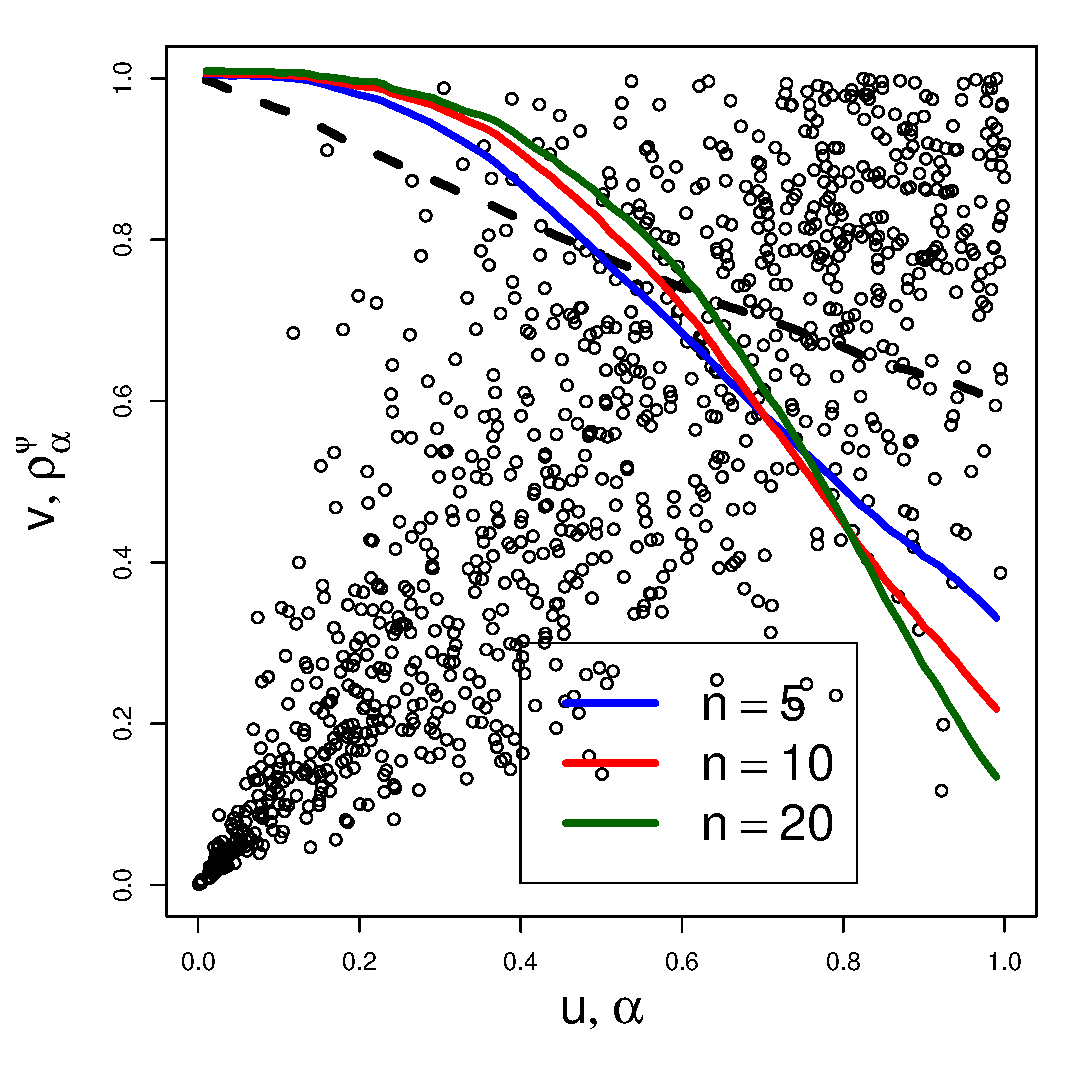
\includegraphics{eml.eps}}
      \resizebox{60mm}{!}{\includegraphics{eml1.eps}} \\
      \resizebox{60mm}{!}{\includegraphics{eml2.eps}}
      \resizebox{60mm}{!}{\includegraphics{eml3.eps}} \\
    \end{tabular}
    \caption{Calculation of generalised layer dependence (coloured lines) assuming $\phi(v)=v^n$ for $n=5$, $10$ and $20$, based on a Clayton copula. Original layer dependence is represented by dotted lines. The top left panel uses the original percentile rank gap, while remaining panels uses the transformed percentile rank gap scale for each value of $n$.}
    \label{fgeneral}
  \end{center}
\end{figure}

\end{comment}



\section{Conclusion}\label{sconclusion}

Layer dependence captures dependence structures in bivariate copulas, and shares the same practical properties as Spearman's correlation. Layer dependence is connected to, and refines, current approaches to measure tail dependence. Taking weighted averages of layer dependence curves yields Spearman's correlation and alternate measures of overall dependence which emphasize different areas of the dependence structure.

Using layer dependence in copula fitting enhances the process by capturing and reflecting the dependence structures in past data, whilst flexibly accommodating expert opinion. 

\newpage


\begin{comment}

\subsection{Simulating constant layer dependence}\label{pconstant}


The following details an approach to simulate $(u,v)$ with constant layer dependence $\ell_\alpha=r$ where $0\leq r\leq 0.5$. First simulate bivariate uniform $(u_*,v_*)$ as
$$
(u_*,v_*)=(z\leq c) \times \{(u_0,v_0)\times c\} +(z>c)\times \{(c,c)+(u_0,v_0)\times (1-c)\}
$$
where $z$, $c$, $u_0$ and $v_0$ are independent uniform. Direct calculation shows the layer dependence of $(u_*,v_*)$ is constant and equal to $0.5$. Hence model $(u,v)$ as a mixture of independent uniform random variables and $(u_*,v_*)$, with weights $1-2r$ and $2r$, respectively. The layer dependence of $(u,v)$ is $(1-2r)\times 0+2r\times 0.5=r$, as desired.
\end{comment}


\newpage

\section{Appendix}


\subsection{Proof of equation \eref{gapexp}}

Since $\E(v)=\alpha\E(v|u\le\alpha)+(1-\alpha)\E(v|u>\alpha)$, the numerator of the middle expression is \eref{gapexp} is
$$
\E(v|u>\alpha)-\E(v|u\leq \alpha) = \E(v|u>\alpha)- \frac{\E(v)-(1-\alpha)\E(v|u>\alpha)}{\alpha}
$$
$$
= \frac{\E(v|u>\alpha)-\E(v)}{\alpha}
= \frac{\E\{vI_\alpha(u)\}-\E(v)\E\{I_\alpha(u)\}}{\alpha(1-\alpha)}
= \frac{\cov\{v,I_\alpha(u)\}}{\alpha(1-\alpha)} \;,
$$
and similarly the denominator is
$$
\E(v|u>\alpha)-\E(v|u\leq \alpha) = \frac{\cov\{u,I_\alpha(u)\}}{\alpha(1-\alpha)} = 0.5 \;,
$$
noting $\cov\{u,I_\alpha(u)\}=0.5\alpha(1-\alpha)$. Combining these two results yields the first and third expressions of \eref{gapexp}. This completes the proof.


\subsection{Proof of equation \eref{decomposition}}

Firstly the measure of discordance is
$$
\gamma_\alpha
=-\frac{\cov\{(u\leq\alpha),(v\leq\alpha)\}}{\var\{(u\leq\alpha)\}}
=\frac{\alpha^2-C(\alpha,\alpha)}{\alpha(1-\alpha)}   \;,
$$
and the measure of dispersion is
$$
\delta_\alpha = 2 \E\left\{(u-v)(u>v)|(u-\alpha)(v-\alpha)<0\right\}
$$
$$
=  \frac{2\E\{(u-v)(u>v)(u>\alpha)(v\leq\alpha)\}}{2\E\{(u>\alpha)(v\leq\alpha)\}}
= \frac{\E\{(u-v)(u>\alpha)(v\leq\alpha)\}}{\alpha-C(\alpha,\alpha)}
$$
$$
= \frac{\E\{(u-v)(u>\alpha)\}-\E\{(u-v)(u>\alpha)(v>\alpha)\}}{\alpha-C(\alpha,\alpha)}
 = \frac{\E\{(u-v)(u>\alpha)\}}{\alpha-C(\alpha,\alpha)} \;.
$$
Substituting the above expressions for $\gamma_\alpha$ and $\delta_\alpha$ into the right hand side of \eref{decomposition} yields the expression for $\ell_\alpha$ in \eref{gapexp}, completing the proof.



\subsection{Proof of coherence properties in section \aref{scoherence}}

\textbf{Independence property}

If $u$ and $v$ are independent, then layer dependence is
$$
\ell_\alpha = \frac{\cov\{v,(u>\alpha)\}}{\cov\{u,(u>\alpha)\}}
=0 \cq  0\leq\alpha\leq 1
$$
since the numerator is zero.


\textbf{Perfect dependence property}

If $u$ and $v$ are comonotonic or $v=u$, then layer dependence
$$
\ell_\alpha = \frac{\cov\{v,(u>\alpha)\}}{\cov\{u,(u>\alpha)\}}= \frac{\cov\{u,(u>\alpha)\}}{\cov\{u,(u>\alpha)\}}
=1 \cq  0\leq\alpha\leq 1  \;.
$$
In addition $\ell_\alpha=1$ implies from \eref{gapexp} $\E(v|u>\alpha)-\E(v|u\le\alpha)=0.5$ for all $\alpha$. Substituting $\E(v|u\le\alpha)= \{\E(v)-(1-\alpha)\E(v|u>\alpha)\}/\alpha$ yields $\E(v|u>\alpha)=0.5(\alpha+1)$. Hence the conditional expectation
$$
\E(v|u=\alpha) = - \frac{\de}{\de\alpha} \left\{(1-\alpha)\E(v|u>\alpha) \right\} = \alpha \cq 0\le\alpha\le 1\; ,
$$
implying $v=u$, completing the proof. A similar proof holds for countermonotonicity where $v=1-u$.

\textbf{Symmetry}

Replacing $v$ with $1-v$ yields layer dependence
$$
\frac{\cov\{1-v,I_\alpha(u)\}}{\cov\{u,I_\alpha(u)\}} =
- \frac{\cov\{v,I_\alpha(u)\}}{\cov\{u,I_\alpha(u)\}} = -\ell_\alpha \;,
$$
whilst replacing $u$ with $1-u$ yields
$$
\frac{\cov\{v,I_\alpha(1-u)\}}{\cov\{1-u,I_\alpha(1-u)\}}
=-\frac{\cov\{v,1-I_{1-\alpha}(u)\}}{\cov\{u,1-I_{1-\alpha}(u)\}}
=-\frac{\cov\{v,I_{1-\alpha}(u)\}}{\cov\{u,I_{1-\alpha}(u)\}}
=-\ell_{1-\alpha} \;.
$$
Using a similar proof, replacing $v$ and $u$ with $1-v$ and $1-u$, respectively, yields layer dependence $\ell_{1-\alpha}$.

\textbf{Correlation order}


If $(u^*,v^*)$ exceeds $(u,v)$ in correlation order, then
$$
\cov\{f(u_*),g(v_*)\} \geq \cov\{f(u),g(v)\}
$$
for any non-decreasing functions $f$ and $g$ \citep{dhaene2009correlation}. Therefore the numerator of layer dependence in \eref{ellalpha} $\cov\{v^*,I_\alpha(u^*)\} \geq \cov\{v,I_\alpha(u)\}$ since $I_\alpha(u)$ is increasing in $u$, and the denominators are the same. Thus $(u^*,v^*)$ has higher layer dependence than $(u,v)$.




\textbf{Bounds}

Since layer dependence preserves correlation order, $\ell_\alpha\le 1$ since $\ell_\alpha=1$ if and only if $u$ and $v$ are comonotonic and comonotonicity represents maximum correlation order \citep{dhaene2009correlation}. Similarly $\ell_\alpha \ge -1$ noting countermonotonicity represents minimum correlation order and leads to $\ell_\alpha=-1$.

\newpage


\section*{References}

\bibliography{PhD}





\end{document}
